%!TEX encoding = UTF-8 Unicode
\documentclass[french, a4paper, 10pt, twocolumn, landscape]{article}



%% Langue et compilation

\usepackage[utf8]{inputenc}
\usepackage[T1]{fontenc}
\usepackage[french]{babel}
\usepackage{lmodern}       % permet d'avoir certains "fonts" de bonne qualite
\renewcommand{\familydefault}{\sfdefault}
%% LISTE DES PACKAGES

\usepackage{mathtools}     % package de base pour les maths
\usepackage{amsmath}       % mathematical type-setting
\usepackage{amssymb}       % symbols speciaux pour les maths
\usepackage{textcomp}      % symboles speciaux pour el text
\usepackage{gensymb}       % commandes generiques \degree etc...
\usepackage{tikz}          % package graphique
\usepackage{wrapfig}       % pour entourer a cote d'une figure
\usepackage{color}         % package des couleurs
\usepackage{xcolor}        % autre package pour les couleurs
\usepackage{pgfplots}      % pacakge pour creer des graph
\usepackage{epsfig}        % permet d'inclure des graph en .eps
\usepackage{graphicx}      % arguments dans includegraphics
\usepackage{pdfpages}      % permet d'insérer des pages pdf dans le document
\usepackage{subfig}        % permet de creer des sous-figure
% \usepackage{pst-all}       % utile pour certaines figures en pstricks
\usepackage{lipsum}        % package qui permet de faire des essais
\usepackage{array}         % permet de faire des tableaux
\usepackage{multicol}      % plusieurs colonnes sur une page
\usepackage{enumitem}      % pro­vides user con­trol: enumerate, itemize and description
\usepackage{hyperref}      % permet de creer des hyperliens dans le document
\usepackage{lscape}        % permet de mettre une page en mode paysage

\usepackage{fancyhdr}      % Permet de mettre des informations en hau et en bas de page      
\usepackage[framemethod=tikz]{mdframed} % breakable frames and coloured boxes
\usepackage[top=1.8cm, bottom=1.8cm, left=1.5cm, right=1.5cm]{geometry} % donne les marges
\usepackage[font=normalsize, labelfont=bf,labelsep=endash, figurename=Figure]{caption} % permet de changer les legendes des figures
\setlength{\parskip}{0pt}%
\setlength{\parindent}{18pt}
\usepackage{lewis}
\usepackage{bohr}
\usepackage{chemfig}
\usepackage{chemist}
\usepackage{tabularx}
\usepackage{pgf-spectra} % permet de tracer des spectres lumineux des atomes et des ions
\usepackage{pgf}

\usepackage{flexisym}
\usepackage{soul}
\usepackage{ulem}
\usepackage{cancel}

\usepackage{import}
\usepackage{physics}
\usepackage[outline]{contour} % glow around text
\tikzset{every shadow/.style={opacity=1}}


%% LIBRAIRIES

\usetikzlibrary{plotmarks} % librairie pour les graphes
\usetikzlibrary{patterns}  % necessaire pour certaines choses predefinies sur tikz
\usetikzlibrary{shadows}   % ombres des encadres
\usetikzlibrary{backgrounds} % arriere plan des encadres


%% MISE EN PAGE

\pagestyle{fancy}     % Défini le style de la page

\renewcommand{\headrulewidth}{0pt}      % largeur du trait en haut de la page
\fancyhead[L]{\textbf{\textcolor{cyan}{Cours}} - Thème 4 - La Terre un astre singulier}         % info coin haut gauche
\fancyhead[R]{\textit{Première Enseignement Scientifique}}  % info coin haut droit

% % bas de la page
% \renewcommand{\footrulewidth}{0pt}      % largeur du trait en bas de la page
% \fancyfoot[L]{}  % info coin bas gauche
\fancyfoot[R]{Lycée GT Jean Guéhenno}                         % info coin bas droit


\setlength{\columnseprule}{1pt} 
\setlength{\columnsep}{30pt}



%% NOUVELLES COMMANDES 

\DeclareMathOperator{\e}{e} % permet d'ecrire l'exponentielle usuellement


\newcommand{\gap}{\vspace{0.15cm}}   % defini une commande pour sauter des lignes
\renewcommand{\vec}{\overrightarrow} % permet d'avoir une fleche qui recouvre tout le vecteur
\newcommand{\bi}{\begin{itemize}}    % begin itemize
\newcommand{\ei}{\end{itemize}}      % end itemize
\newcommand{\bc}{\begin{center}}     % begin center
\newcommand{\ec}{\end{center}}       % end center
\newcommand\opacity{1}               % opacity 
\pgfsetfillopacity{\opacity}

\newcommand*\Laplace{\mathop{}\!\mathbin\bigtriangleup} % symbole de Laplace

\frenchbsetup{StandardItemLabels=true} % je ne sais plus

\newcommand{\smallO}[1]{\ensuremath{\mathop{}\mathopen{}o\mathopen{}\left(#1\right)}} % petit o

\newcommand{\cit}{\color{blue}\cite} % permet d'avoir les citations de couleur bleues
\newcommand{\bib}{\color{black}\bibitem} % paragraphe biblio en noir et blanc
\newcommand{\bthebiblio}{\color{black} \begin{thebibliography}} % idem necessaire sinon bug a cause de la couleur
\newcommand{\ethebiblio}{\color{black} \end{thebibliography}}   % idem
%%% TIKZ


%% COULEURS 


\definecolor{definitionf}{RGB}{220,252,220}
\definecolor{definitionl}{RGB}{39,123,69}
\definecolor{definitiono}{RGB}{72,148,101}

\definecolor{propositionf}{RGB}{255,216,218}
\definecolor{propositionl}{RGB}{38,38,38}
\definecolor{propositiono}{RGB}{109,109,109}

\definecolor{theof}{RGB}{255,216,218}
\definecolor{theol}{RGB}{160,0,4}
\definecolor{theoo}{RGB}{221,65,100}

\definecolor{avertl}{RGB}{163,92,0}
\definecolor{averto}{RGB}{255,144,0}

\definecolor{histf}{RGB}{241,238,193}

\definecolor{metf}{RGB}{220,230,240}
\definecolor{metl}{RGB}{56,110,165}
\definecolor{meto}{RGB}{109,109,109}


\definecolor{remf}{RGB}{230,240,250}
\definecolor{remo}{RGB}{150,150,150}

\definecolor{exef}{RGB}{240,240,240}

\definecolor{protf}{RGB}{247,228,255}
\definecolor{protl}{RGB}{105,0,203}
\definecolor{proto}{RGB}{174,88,255}

\definecolor{grid}{RGB}{180,180,180}

\definecolor{titref}{RGB}{230,230,230}

\definecolor{vert}{RGB}{23,200,23}

\definecolor{violet}{RGB}{180,0,200}

\definecolor{copper}{RGB}{217, 144, 88}

%% Couleur des ref

\hypersetup{
	colorlinks=true,
	linkcolor=black,
	citecolor=blue,
	urlcolor=black
		   }

%% CADRES

\tikzset{every shadow/.style={opacity=1}}

\global\mdfdefinestyle{doc}{backgroundcolor=white, shadow=true, shadowcolor=propositiono, linewidth=1pt, linecolor=black, shadowsize=5pt}
\global\mdfdefinestyle{titr}{backgroundcolor=metf, shadow=true, shadowcolor=propositiono, linewidth=1pt, linecolor=black, shadowsize=5pt}
\global\mdfdefinestyle{theo}{backgroundcolor=theof, shadow=true, shadowcolor=theoo, linewidth=1pt, linecolor=theol, shadowsize=5pt}
\global\mdfdefinestyle{prop}{backgroundcolor=theof, shadow=true, shadowcolor=propositiono, linewidth=1pt, linecolor=theol, shadowsize=5pt}
\global\mdfdefinestyle{def}{backgroundcolor=definitionf, shadow=true, shadowcolor=definitiono, linewidth=1pt, linecolor=definitionl, shadowsize=5pt}
\global\mdfdefinestyle{histo}{backgroundcolor=histf, shadow=true, shadowcolor=propositiono, linewidth=1pt, linecolor=black, shadowsize=5pt}
\global\mdfdefinestyle{avert}{backgroundcolor=white, shadow=true, shadowcolor=averto, linewidth=1pt, linecolor=avertl, shadowsize=5pt}
\global\mdfdefinestyle{met}{backgroundcolor=metf, shadow=true, shadowcolor=meto, linewidth=1pt, linecolor=metl, shadowsize=5pt}
\global\mdfdefinestyle{rem}{backgroundcolor=metf, shadow=true, shadowcolor=meto, linewidth=1pt, linecolor=metf, shadowsize=5pt}
\global\mdfdefinestyle{exo}{backgroundcolor=exef, shadow=true, shadowcolor=propositiono, linewidth=1pt, linecolor=exef, shadowsize=5pt}
\global\mdfdefinestyle{not}{backgroundcolor=definitionf, shadow=true, shadowcolor=propositiono, linewidth=1pt, linecolor=black, shadowsize=5pt}
\global\mdfdefinestyle{proto}{backgroundcolor=protf, shadow=true, shadowcolor=proto, linewidth=1pt, linecolor=protl, shadowsize=5pt}

%%%%%%
\definecolor{cobalt}{rgb}{0.0, 0.28, 0.67}
\definecolor{applegreen}{rgb}{0.55, 0.71, 0.0}

\usepackage{tcolorbox}
  \tcbuselibrary{most}
  \tcbset{colback=cobalt!5!white,colframe=cobalt!75!black}



\newtcolorbox{definition}[1]{
	colback=applegreen!5!white,
  	colframe=applegreen!65!black,
	fonttitle=\bfseries,
  	title={#1}}
\newtcolorbox{Programme}[1]{
	colback=cobalt!5!white,
  	colframe=cobalt!65!black,
	fonttitle=\bfseries,
  	title={#1}} 
\newtcolorbox{Proposition}[1]{
      colback=theof,%!5!white,
        colframe=theol,%!65!black,
      fonttitle=\bfseries,
        title={#1}}  

\newtcolorbox{Exercice}[1]{
  colback=cobalt!5!white,
  colframe=cobalt!65!black,
  fonttitle=\bfseries,
  title={#1}}  

\newtcolorbox{Resultat}[1]{
	colback=theof,%!5!white,
	colframe=theoo!85!black,
  fonttitle=\bfseries,
	title={#1}} 	

  \setlength{\tabcolsep}{20pt}

  \renewcommand{\arraystretch}{1.5}
  
  \newcommand{\pisteverte}{
	\begin{flushleft}
		\begin{tikzpicture}
			\draw (0,0) -- (0,.2);
			\draw[fill = green] (0,0.4) circle (0.2);
			\node[draw] at (1.5,0.3) {Piste verte};
		\end{tikzpicture}
		\end{flushleft}
}

\newcommand{\pistebleue}{
	\begin{flushleft}
		\begin{tikzpicture}
			\draw (0,0) -- (0,.2);
			\draw[fill = blue] (0,0.4) circle (0.2);
			\node[draw] at (1.5,0.3) {Piste bleue};
		\end{tikzpicture}
		\end{flushleft}
}
\newcommand{\pistenoire}{
	\begin{flushleft}
		\begin{tikzpicture}
			\draw (0,0) -- (0,.2);
			\draw[fill = black!80] (0,0.4) circle (0.2);
			\node[draw] at (1.5,0.3) {Piste noire};
		\end{tikzpicture}
		\end{flushleft}
}
  \newcommand{\titre}[1]{
    \begin{mdframed}[style=titr, leftmargin=0pt, rightmargin=0pt, innertopmargin=8pt, innerbottommargin=8pt, innerrightmargin=10pt, innerleftmargin=10pt]
      \begin{center}
        \Large{\textbf{#1}}
      \end{center}
    \end{mdframed}
  }


  %% COMMANDE Exercice
  
  \newcommand{\exo}[3]{
    \begin{mdframed}[style=exo, leftmargin=0pt, rightmargin=0pt, innertopmargin=8pt, innerbottommargin=8pt, innerrightmargin=10pt, innerleftmargin=10pt]
  
      \noindent \textbf{Exercice #1 - #2}\medskip
  
      #3
    \end{mdframed}
  }
  
     
  \newcommand{\questions}[1]{
    \begin{mdframed}[style=exo, leftmargin=0pt, rightmargin=0pt, innertopmargin=8pt, innerbottommargin=8pt, innerrightmargin=10pt, innerleftmargin=10pt]
  
      \noindent \textbf{Questions :}\smallskip
  
      #1
    \end{mdframed}
  }
  
  \newcommand{\doc}[3]{
    \begin{mdframed}[style=doc, leftmargin=0pt, rightmargin=0pt, innertopmargin=8pt, innerbottommargin=8pt, innerrightmargin=10pt, innerleftmargin=10pt]
  
      \noindent \textbf{Document #1 - #2}\medskip
  
      #3
    \end{mdframed}
  }
\def\width{12}
\def\hauteur{5}


\usetikzlibrary{intersections}
\usetikzlibrary{decorations.markings}
\usetikzlibrary{angles,quotes} % for pic
\usetikzlibrary{calc}
\usetikzlibrary{3d}
\contourlength{1.3pt}

\tikzset{>=latex} % for LaTeX arrow head
\colorlet{myred}{red!85!black}
\colorlet{myblue}{blue!80!black}
\colorlet{mycyan}{cyan!80!black}
\colorlet{mygreen}{green!70!black}
\colorlet{myorange}{orange!90!black!80}
\colorlet{mypurple}{red!50!blue!90!black!80}
\colorlet{mydarkred}{myred!80!black}
\colorlet{mydarkblue}{myblue!80!black}
\tikzstyle{xline}=[myblue,thick]
\def\tick#1#2{\draw[thick] (#1) ++ (#2:0.1) --++ (#2-180:0.2)}
\tikzstyle{myarr}=[myblue!50,-{Latex[length=3,width=2]}]
\def\N{90}

\tikzset{
  % style to apply some styles to each segment of a path
  on each segment/.style={
    decorate,
    decoration={
      show path construction,
      moveto code={},
      lineto code={
        \path [#1]
        (\tikzinputsegmentfirst) -- (\tikzinputsegmentlast);
      },
      curveto code={
        \path [#1] (\tikzinputsegmentfirst)
        .. controls
        (\tikzinputsegmentsupporta) and (\tikzinputsegmentsupportb)
        ..
        (\tikzinputsegmentlast);
      },
      closepath code={
        \path [#1]
        (\tikzinputsegmentfirst) -- (\tikzinputsegmentlast);
      },
    },
  },
  % style to add an arrow in the middle of a path
  mid arrow/.style={postaction={decorate,decoration={
        markings,
        mark=at position .5 with {\arrow[#1]{stealth}}
      }}},
}



\usetikzlibrary{3d, shapes.multipart}

% Styles
\tikzset{>=latex} % for LaTeX arrow head
\tikzset{axis/.style={black, thick,->}}
\tikzset{vector/.style={>=stealth,->}}
\tikzset{every text node part/.style={align=center}}
\usepackage{amsmath} % for \text
 
\usetikzlibrary{decorations.pathreplacing,decorations.markings}

%% MODIFICATION DE CHAPTER  
\makeatletter
\def\@makechapterhead#1{%
  %%%%\vspace*{50\p@}% %%% removed!
  {\parindent \z@ \raggedright \normalfont
    \ifnum \c@secnumdepth >\m@ne
        \huge\bfseries \@chapapp\space \thechapter
        \par\nobreak
        \vskip 20\p@
    \fi
    \interlinepenalty\@M
    \Huge \bfseries #1\par\nobreak
    \vskip 40\p@
  }}
\def\@makeschapterhead#1{%
  %%%%%\vspace*{50\p@}% %%% removed!
  {\parindent \z@ \raggedright
    \normalfont
    \interlinepenalty\@M
    \Huge \bfseries  #1\par\nobreak
    \vskip 40\p@
  }}
  
  \newcommand{\isotope}[3]{%
     \settowidth\@tempdimb{\ensuremath{\scriptstyle#1}}%
     \settowidth\@tempdimc{\ensuremath{\scriptstyle#2}}%
     \ifnum\@tempdimb>\@tempdimc%
         \setlength{\@tempdima}{\@tempdimb}%
     \else%
         \setlength{\@tempdima}{\@tempdimc}%
     \fi%
    \begingroup%
    \ensuremath{^{\makebox[\@tempdima][r]{\ensuremath{\scriptstyle#1}}}_{\makebox[\@tempdima][r]{\ensuremath{\scriptstyle#2}}}\text{#3}}%
    \endgroup%
  }%

\makeatother


\definecolor{darkpastelgreen}{rgb}{0.01, 0.75, 0.24}
\newcommand{\mobiliser}{
  % \begin{flushleft}
    \begin{tikzpicture}[scale=0.6]
      % \draw (0,0) -- (0,.2);
      \draw[color = darkpastelgreen, fill = darkpastelgreen] (0,-0.3) circle (0.3)node[white]{M};
      % \node[draw, white] at (0,-0.3) {\textbf{M}};
    \end{tikzpicture}
    % \end{flushleft}
}

\newcommand{\realiser}{
  % \begin{flushleft}
    \begin{tikzpicture}[scale=.6]
      % \draw (0,0) -- (0,.2);
      \draw[color = blue, fill = blue] (0,-0.3) circle (0.3) node[white]{R};
      % \node[draw, white] at (0,-0.3) {\textbf{R}};
    \end{tikzpicture}
    % \end{flushleft}
}

\definecolor{bostonuniversityred}{rgb}{0.8, 0.0, 0.0}

\newcommand{\analyser}{
  % \begin{flushleft}
    \begin{tikzpicture}[scale=.6]
      % \draw (0,0) -- (0,.2);
      \draw[color = bostonuniversityred, fill = bostonuniversityred] (0,-0.3) circle (0.3) node[white]{A};
      % \node[draw, white] at (0,-0.3) {\textbf{A}};
    \end{tikzpicture}
    % \end{flushleft}
}
\definecolor{amethyst}{rgb}{0.6, 0.4, 0.8}

\newcommand{\communiquer}{
  % \begin{flushleft}
    \begin{tikzpicture}[scale=.6]
      % \draw (0,0) -- (0,.2);
      \draw[color = amethyst, fill = amethyst] (0,-0.3) circle (0.3) node[white]{C};
      % \node[draw, white] at (0,-0.3) {\textbf{C}};
    \end{tikzpicture}
    % \end{flushleft}
}

\newcommand{\applicationnumerique}{\textbf{A.N.:}}

\usepackage{esint}
\usepackage{breqn}
\usepackage{colortbl}
\newcommand{\objectifs}[1]{
	\begin{minipage}{.02\textheight}
	\rotatebox{90}{\textbf{\large Objectifs}}
	\end{minipage}
	\begin{minipage}{.9\linewidth}
			#1 
	\end{minipage}
}
%%
%%
%% DEBUT DU DOCUMENT
%%

\begin{document}

\section*{Leçon 6: Premier principe de la thermodynamique}

\hrulefill\\

\noindent\underline{\textbf{Niveau:}}
\begin{itemize}
  \item CPGE 
\end{itemize}
\underline{\textbf{Pr{\'e}-requis: }}

\begin{itemize}  
  \item Gaz parfait;
  \item travail mécanique; 
  \item notion de système et d’équilibre thermodynamique;
  \item  transformations classiques en thermodynamique.
\end{itemize}
\underline{\textbf{Bibliographie:}}

\begin{itemize}
  \item Dunod PCSI;
%   \item Perez mécanique Chapitre gravitation.
\end{itemize}
\hrulefill

\section*{Introduction}

La thermodynamique est l'étude des propriétés macroscopique d'un système ($P,V,T,...$) sans se préoccuper des processus microscopiques sous-jacents. Elle s'applque donc aux systèmes contenant suffisamment de particules pour que les fluctuations microscopiques puissent être négligées.  C'est une théorie axiomatique basée sur principalement sur deux principes. Animation : \url{https://phet.colorado.edu/sims/html/energy-forms-and-changes/latest/energy-forms-and-changes\_en.html}. 
  
  Pour un système isolé (ni échange d'énergie, ni échange de matière avec l'extérieur), l'énergie ne se créé pas et ne disparaît pas, mais elle se transforme d'une forme à une autre : Ex animation : conversion énergie mécanique-électrique, électrique-thermique. \\
  Si le système est isolé, il y a conservation de l'énergie.

\section*{1. Les transformations dans un système thermodynamique (Dunod)}

\subsection*{1.1. Système thermodynamique}

On appelle système thermodynamique tout système constituté d'un très grand nombre de particules microscopiques. Choisir un système c'est partagé le monde en deux: d'une part le système choisi qui occupe un certain volume $V$ constitué de $N$ particules et d'autre part le reste de l'univers que l'on dénomme \textbf{extérieur}. Le système peut être fermé (pas d'échange de matière), isolé (pas d'échange de matière et d'énergie), ou ouvert.

L'état du système est définit par des variables d'état. Ce sont des grandeurs macroscopiques tels que la température, la pression et le volume,... On distingue deux types de variables. Les variables \textbf{extensives} (dont la valeur est la somme de chaque sous-système comme la masse, elle dépend de la taille du système) et \textbf{intensives} (si elle est la même dans chaque sous-système alors c'est la même pour le système total comme la température, ne dépend pas de la taille du système).

\subsection*{1.2. Énergie interne}

On peut distingueur deu types d'énergie lors de la description d'un système:
\begin{enumerate}
    \item l'énergie interne (microscopique):
C'est la somme des énergies de toutes les particules qui composent le système dans le référnetiel du centre de masse du système. \textbf{énergie cinétique} (translation, rotation, vibrations); \textbf{énergie potentielle d'intéractions entre particules} (liaison covalents, VdW, liaisons ioniques, liaisons métalliques...); \textbf{énergie de masse} ($mc^2$); \textbf{énergie potentielle des particules soumises à une force extérieure}.
    \item énergie macroscopique:

C'est l'énergie cinétique de l'ensemble du système lorsque son centre de masse n'est pas immobile.
\end{enumerate}

En général, en thermodynamique, on se place  dans le référentiel du centre de masse, de sorte que l'on peut éliminer des équations l'énergie cinétique macroscopique. Par contre, si le système est soumis à des forces extérieures, on ne peut pas a priori les éliminer, et elles se manifestent via l'énergie potentielle des particules individuelles.  Cependant si le système est suffisamment petit par rapport à la distance sur laquelle la force considérée varie, alors toutes les particules subissent approximativement la même force et le même potentiel: 

\begin{equation}
    E_{\rm tot} = E_{\rm cin}^M+E_{\rm pot}^M + U
\end{equation}

\subsection*{1.3. Le travail}

C'est une quantité d'énergie échangée entre le milieu considéré et le milieu extérieur. On note le travail $W$. Si $W>0$, le système reçoit de l'énergie. Si $W<0$ il cède de l'énergie. Le travail mécanique s'écrit : $\delta W=\vec{F}\cdot \vec{dr}$.

\textbf{exemple:} les travail des forces de pression.
Faire un schéma, d'un volume de gaz séparé du milieu extérieur par un piston.
\begin{equation}
    \delta W = -P_{\rm ext}\vec{dS}\cdot\vec{dr}=-PdV.
\end{equation} 

On peut commenter différents cas, pression constante, volume constant...
\subsection*{La chaleur}

Un système thermo peut recevoir de l'énergie sans l'intervention d'une action mécanique mesurable à l'échelle macroscopique. Ce transfert d'énergie complémentaire du travail mécanique s'appelle transfert thermique. La chaleur se transfère spontanément du corps chaud au corps froid. La conversion de chaleur en travail mécanique a permis la rev industrielle par la machine à vapeur.


\section*{2. Principe de conservation de l'énergie}

\subsection*{2.1 . Premier principe de la thermodynamique}

La variation de l'énergie interne $U$ d'un système est égale à l'énergie qu'il a reçu sous la forme de travail et de chaleur.

\begin{equation}
    dU + dE_{\rm cin}+dE_{\rm pot}=\delta W+\delta Q
\end{equation}

Dans le référentiel du centre de masse:

 \begin{equation}
     dU = \delta W + \delta Q \leftrightarrow \Delta U = W +Q.
 \end{equation}

\subsection*{2.2. L'enthalpie}

On peut définir une autre fonction d'état du système thermodynamique: l'enthalpie.
\begin{equation}
    H=U+PV
\end{equation}

\subsection*{2.3. Capacité thermique}
 
On appelle capcité thermique à volume constant d'un système fermé $\sigma$ la grandeur $C_v$ telle que la variation $U$ de l'énergie interne du système lorsque la température varie de $dT$, le volume restant constant, est : 

\begin{equation}
    dU = C_vdT.
\end{equation}

$C_v$ se  esure en $J\cdot K^{-1}$. Il s'agit d'une grandeur extensive et additive. Pour un échantillon de coprs pur, dont la taille est donnée par la quantité de matière $n$ se calcule par:

\begin{equation}
    C_v=nC_{vm}
\end{equation}

où $C_{vm}$ est la capacité thermique molaire à volume constant.\medskip

\textbf{cas du gaz parfait:} $U = \frac{3}{2}nRT$, donc $C_v=\frac{3}{2}nR$.\medskip

Dans le cas d'un système fermé à pression constante:

\begin{equation}
    dH = C_p dT
\end{equation}

Dans le cas d'un gaz parfait: 

\begin{equation}
    Cp-Cv=nR,~Cv = \dfrac{nR}{\gamma -1},~Cp = \dfrac{R\gamma}{\gamma-1}
\end{equation}

\section*{3. Applications expérimentales}

\subsection*{3.1. Détermination d'une capacité thermique massique (Dunod PCSI p756  Chap 26 2021)}

\doc{1}{Liste du matériel}{
\begin{itemize}
\item thermomètre;
\item calorimètre;
\item Eau;
\item éprouvette;
\item balance;
\item bain thermostaté;
\item masselotte attachée à un fil;
\item plaque chauffante ou bouilloire.
\item morceau de fer, laiton $m\sim 100 g$
\item agitateur pour homogénéiser le mélange
\end{itemize}
}

\noindent\underline{\textbf{Mesure de l'équivalent en eau du calorimètre}}

On pose le calorimètre sur la balance, on ajoute un volume de 80g d'eau à température ambiante. Il faut laisser le calorimètre avec l'eau se thermalisé quelques minutes. On mesure la température $T_{froid}$ et la masse de l'eau dans le calorimètre $m_{ini}$. On fait bouillir de l'eau on mesure sa température $T_{chaud}$  et on ajoute $80g$ d'eau chaude dans le calorimètre.  On mesure la température à l'équilibre $T_{eq}$.

Bilan du mélange : $\Delta H = 0 $ 
$$0 = m_{f}c_{eau}(T_{eq}-T_{if})+m_{\rm c}c_{eau}(T_{eq}-T_{ic})+m_{\rm cal}c_{eau}(T_{eq}-T_{if}).$$ 
$$m_{cal} = -\dfrac{m_{f}(T_{eq}-T_{if})+m_{\rm c}c_{eau}(T_{eq}-T_{ic})}{T_{eq}-T_{if}).}$$


\noindent\underline{\textbf{Mesure de la capacité calorifique d'un échantillon de métal}}

On verse dans le calorimètre ($m_c$), une masse $m_{ef}$ d'eau très froide et on mesure la température qui se stabilise après quelques instants. On trouve une température $\theta_0$. On introduit dans le calorimètre l'échantillon de fer, que l'on a pesé ($m_{\rm fer}$) et qui est initialement à la température d'une étuve thermostatée à une température $\theta_{fer}$. On attend que la température se stabilise et on mesure la température finale $\theta_f$.

\begin{equation}
    \Delta H = 0 = \Delta H_{eau}+\Delta H_{cal} + \Delta H_{fer}
\end{equation}

\begin{equation}
    m_{\rm eau}c_{\rm eau}(\theta_f - \theta_0)+m_{\rm cal}c_{\rm eau}(\theta_f - \theta_0) + m_{\rm fer}c_{\rm fer}(\theta_f-\theta_{fer})=0
\end{equation}



On en déduit : $c_{\rm fer}=\dfrac{c_{\rm eau}(m_{\rm eau}+m_{\rm cal})(T_{f}-\theta_0)}{m_{\rm fer}(\theta_f-\theta_{\rm fer})}\rm =\dots ~J.kg^{-1}.K^{-1}$ à comparer à $c_{\rm fer}=449$~J.kg$^{-1}$.K$^{-1}$.
\subsection*{3.2. Détente de Joule Gay Lussac}


Deux enceintes séparées par un robinet. Une enceinte est remplie par un gaz, l'autre par un fluide. Ces enceintes sont calorifugées et avec des parois rigides. On ouvre le robinet. \\
  Système = {gaz+vide+enceintes}. On a $\Delta U=0$. Si $U(T)$ (première loi de Joule) : $\Delta U = C_{V}\Delta T = 0$ donc transformation isotherme. \\
  Cette expérience permet de vérifier si un gaz vérifie la première loi de Joule en mesurant la variation de température.
  

\section*{Conclusion}

Dans cette leçon, on a parlé du premier principe qui est un principe de conservation de conservation. Ce principe est complété par le second principe, qui lui, est plutôt un principe d'évolution et qui porte sur le caractère réversible ou irréversible d'une transformation. Pour finir, ces principes et la thermodynamique classique en général a été formalisée plus tard par la mécanique statistique qui permet d'expliquer les résultats de la thermodynamiques en faisant le lien entre l'échelle microscopique et macroscopique.


\questions{

\textbf{C : Sur la vidéo, comment on fait conversion énergie mécanique et électrique ?}  \textcolor{purple}{Avec un alternateur : un aimant est entrainé par l'énergie mécanique qui créé un courant variable dans une bobine par induction. Exemple : une dynamo de bicyclette. Si pas de champs magnétiques préexistant, induction électromagnétique.} \newline
  
  \textbf{C : Dans l'énoncé du premier principe, quelles sont les particularités de A et B ?}  \textcolor{purple}{Ils sont à l'équilibre thermodynamique pour qu'on puisse leur défiir une énergie .} \newline
  
  \textbf{C : W est le travail des forces non conservatives ? Si je prends un piston qui est bloqué par un poids, il y a le poids dans W ? Si j'ajoute une force, ça agit sur E$_p$ par sur U (par exemple la force de Lorentz qui agit sur chaque particule ?}  \textcolor{purple}{Il est bien présent dans la partie gauche de l'équation. Si on le met à doite ça agit sur $E_p$ et on met un signe \og - \fg. C'est un peu indifférent de le mettre à droite où à gauche mais il ne faut pas le compter deux fois et mettre le bon signe. } \newline
  
  \textbf{C : De façon non ambigüe, peut-on mesurer une quantité de chaleur ou savor ce que c'est ?}  \textcolor{purple}{La chaleur ça sera toute la variation d'énergie sauf le travail des forces macroscopiques. On peut mesurer la variation d'énergie interne dans certaines conditions.} \newline
  
  \textbf{C :Si transfo quasi-statique, on peut faire $-P_edV$. Peut-on juste dire que la transformation est réversible ?}  \textcolor{purple}{Oui ça fonctionne mais dans la vie il n'existe pas de transformation réversible.} \newline
  
  \textbf{C : Définition de réversible ?}  \textcolor{purple}{On peut changer le sens et changeant infiniment peu les contraintes extérieures. On peut prendre l'exemple d'un piston où il y a des frottements pour la différence entre réversible et quasi-statique.} \newline
  
  \textbf{C : Dans la détente Joule Gay Lussac, est-ce que c'est important que l'enceinte soit vide ou remplie d'un gaz à pression plus faible par exemple ?}  \textcolor{purple}{Il faut juste faire attention à la définition du système. } \newline
  
  \textbf{C :Si on veut une variation de chaleur $\delta Q$ pour un fluide, quels sont les coefficients importants ?}  \textcolor{purple}{Il y a 6 variables calorimétriques importantes. Suivant le système, il faut prendre la dépendance en volume etc... On peut montrer qu'il n'y en a que deux d'indépendantes.} \newline
  
  \textbf{C :Différentes façon d'exprimer $\delta Q$ : $\delta Q = c_vdT + ldV = c_pdT + hdP = \lambda dP + \mu dV$. On peut montrer la relation entre pente adiabatique et pente isotherme. Quelle est la pente la plus importante entre une adiabatique ou une isotherme dans le diagramme (P,V) ? Calculer la pente pour une adiabatique et une isotherme ? }  \textcolor{purple}{Isotherme : $dT=0$ donc $\delta Q= ldV = hdP$. Adiabatique : $dV = -\frac{c_v}{l}dT$ et $dP = -\frac{c_p}{h}dT= \frac{c_pl}{hc_v}dV$.} \newline
  
  \textbf{C :Comment exprimer de manière générale $dP$ en fonction de $dT$ et $dV$ à partir d'une équation d'état ?}  \textcolor{purple}{$dT = (\frac{\partial{T}}{\partial{P}})_VdP + (\frac{\partial{d}T}{\partial{d}V})_VdV$. On en déduit } \newline
  
  \textbf{C :Dans le diagramme (P,V), on considère des transformations infinitésimales entre A et D (entre A et B : isochore, B et C : isobare, C et D : isotherme et entre D et A : isobare). Calculer la variation infinitésimale $\delta Q$ sur le cycle en commençant d'abord par les chemins A-B-C et A-D-C.}  \textcolor{purple}{Sur A-B-C : $\delta Q = \lambda dP + \mu dV$. Sur A-D-C, $\delta Q = c_pdT + hdP$. Donc sur le cycle : $\delta Q = -\delta W = \lambda dP + \mu dV - c_pdT - hdP$. } \newline
}

\clearpage

\section*{Leçon 7: Transition de phase}

\hrulefill\\

\noindent\underline{\textbf{Niveau:}}
\begin{itemize}
  \item CPGE 
\end{itemize}
\underline{\textbf{Pr{\'e}-requis: }}

\begin{itemize}
  \item notion de système et d’équilibre thermodynamique;
  \item  transformations classiques en thermodynamique;
  \item premier et second principe.
\end{itemize}
\underline{\textbf{Bibliographie:}}

\begin{itemize}
  \item Thermodynamique de Diu;
  \item Thermodynamique de Pérez;
  \item thermodynamique BFR.
  \item Tout en un ancien programme N. Choimet. Thermodynamique. PC-PSI. Bréal, 2001
  \item J.-M. Donnini and L. Quaranta. Dictionnaire de physique expérimen-
  tale. Tome 2 : thermodynamique et applications. Pierron, 1997
  \item Jerôme Beugnon : \url{https://www.lkb.upmc.fr/boseeinsteincondensates/wp-content/uploads/sites/10/2017/10/CoursThermo2017.pdf}
\end{itemize}
\hrulefill

\section*{Introduction}
La notion de phase paraît assez naturelle si on prend l’exemple de l’eau. La glace, la vapeur et l’eau liquide sont toutes trois des phases dans lequel l’arrangement des molécules d’eau n’est pas du tout la même d’une phase à une autre. Un corp peut suivant les conditions qui lui sont imposées se présenter sous différentes phases (états) tel que solide, liquide ou vapeur. Dans les chapitres précédents, nous avons abordé les corps purs dans une phase unique. Dans cette leçon, je vous propose d'analyser le passage d'une phase à une autre appelée changement d'état et d'examiner les conditions de coexistence entre plusieurs phases.

\section*{1. Une transition du premier ordre solide/liquide}

\subsection*{1.1. Manipulation : Mono-variance de l'équilibre liquide solide de l'étain}

On réalise la manipulation dans le poly de philippe, on mesure la température de fusion de l'étain.
On osberve le palier de température caractéristique d'une transition de phase du premier ordre. 

\subsection*{1.2. Diagramme des variables d'états}

\subsubsection*{1.2.1 Calcul de la variance (Diu p373)}

Les variables intensives jouent un rôle essentiel elles caractérisent les propriétés intrinsèques du mélange indépendamment de la masse dans les différentes phases. En thermodynamique on définit la variance ou le nombre de degrés de liberté tel que : 
\begin{equation}
  v = \text{nb de facteurs d'équilibre} - \text{nb de relations}
\end{equation}

Les facteurs d'équilibres sont : la température, la pression ainsi que le nombre $n$ d'espèces chimiques dans les $\phi$ phases. On a donc $$\text{nb de facteurs d'équilibre} = 2+n\phi$$

Le nombre de relations est donnée par: 
\begin{itemize}
  \item pour chaque phase $\sum_i x_i^\phi =1$, ona donc $\phi relations$
  \item à l'équilibre $\mu_i^{\alpha}=\mu_i^\beta=...=\mu_i^\phi$ ce qui donne $\phi-1$ relations, soit pour $n$ espèces $n(\phi-1)$
  \item Si relation chimique : $\sum_i\pm\nu_i\mu_i=0$
\end{itemize}

\begin{equation}
  v = 2+n\phi-(\phi+n(\phi-1)+r)= 2+n-\phi-r
\end{equation}

Pour un corp pur, dans le cas de la transition liquide solide. Au cours de la transition où les phases liquide et solide coexistent. On suppose l'équilibre entre les deux phases établies. Dans ce cas $r=0$, $\phi= 2$ $n=1$. On a donc $v=1$. À P fixé, la température ne peut pas varier.

\subsubsection*{1.2.2. Interprétation sur un diagramme (P,T)}

On montre le diagramme (P,T) dans le Diu p297 , on lit sur le diagramme la transition liquide solide. On a l'impression que lorsque T augmente que l'on passe d'un coup de solide à liquide (On peut illustrer avec l'expérience du Bouillant de Franklin). Mais ce ce n'est pas le cas la transition est continue. On a une évolution du volume qui permet le passage continue d'une phase à l'autre. Montrer le diagramme de Clapeyron (P,V) et les isothermes\medskip

Transformation à température constante. On a une enceinte avec un piston mobile. On considère une transformation quasi-statique et isotherme. On voit apparaître à une certaine pression PS du liquide qu’on définit comme la pression de vapeur saturante. Si on continue à appuyer, la pression reste constante jusqu’à ce que tout le gaz se soit transformer en liquide. Si on répète la même expérience à une température différente, la pression PS va changer.


\textcolor{red}{Transition : } Comment décrire thermodynamiquement ce qui se passe au niveau de ce changement d'état ? Comme on travaille à P ou T variable, on va utiliser l'enthalpie libre $G = U+PV-TS$.
  

\subsection*{1.3. Description thermodynamique de l'équilibre}

\subsubsection*{1.3.1. Transition ponctuelle dans le diagramme}

Afin de décrire la transformation, le potentiel thermodynamique le plus adapté est l'enthalpie libre car :

\begin{equation}
  dG=VdP-SdT+\mu dN
\end{equation}

Sur slide on donne le calcul pour arriver à l'expression de l'enthalpie libre que l'on cherche à minimiser. On décrit le cas où $G1=G2$. Dans ce cas le potentiel thermo est constant quelque soit la composition du système thermodynamique. Les deux phases coexistent en proprotion arbitraires. Un faible apport d'énergie permet de basculer de l'un à l'autre.  Il s'agit d'une transformation du premier ordre. Continuité de G, dérivées premières discontinue. 

\subsubsection*{1.3.2.Relation de Clapeyron}

Pendant le changement d'état il ya variation de S et V. La chaleur latente de transition est liée à la discontinuité de l'entropie et du volume. C'est la quantité de chaleur que le système doit recevoir pour passer de la basse entropie à la haute entropie en suivant le palier de transition. 

\begin{equation}
  S_B-S_A=\dfrac{\partial p_{AB}}{\partial T_{AB}}(V_B-V_A).
\end{equation}

La courbe $p=p(T)$ est l'équation de la  courbe du diagramme (P,T). Cette équation donne le coût énergétique  de la transition de phase. 

\subsection*{1.3.3. Retard à la transition de phase: métastabilité}

Manipulation avec la surfusion de l'acide acétique dans le poly de philippe. C'est la tension de surface qui coûte de l'énergie au système et qui est responsable du retard à la transition.

% \section{Transitions solide-liquide-vapeur}

% \subsection{Diagrammes des variables d'état Diu p300/314}



% On présente les courbes (T,p), (V,p) et (p,V,T) sur slides. D'ecrire les courbes et le point triple ( en ce point le corps pur est en équilibre sous ses trois phases)


% \textbf{(Diu p373)} On écrit le calcul de la variance pour un coups pur diphasique à l'équilibre.  On donne les relations entre les paramètres et les potentiels chimiques.  On trouve que la variance est égale à 1. On peut alors interpréter sur la courbe vaporistion (p,T).

% On constate l'éxistence des 3 phases sur le diagramme, les frontières représentent tous les états de coexistence des 2 phases à $T$ et $P$.  Présence du point triple et le justifier avec la variance (Diu p374). 

% \textbf{Expérience de Bouillant de Franklin:}\url{https://www.youtube.com/watch?v=nxAdQ_8tC1U} Permet d'expliquer comment on se déplace sur le diagramme P,T.\medskip

% En regardant ce qu'il se passe lorsqu'on augmente la température on aurait envie de dire que l'eau passe subitement du liquide à la vapeur... ce qui n'arrive pas en réalité: Les proportions de chaque phase varie continuement ! On a besoin du diagramme de \textbf{Clapeyron} (P,V). Présenter en slide les diagrammes (P,V) puis 3D. On peut finalement montrer le diagramme $L,V$ qui mermet de constater les différentes phases, le point critique et les isothermes.

% \textbf{Transition:} on peut connaître la composition d'un système à partir de la connassance de P,V,T et de diagrammes P,T et P,V. mais comment décrire thermodynamiquement les transformations.
% \subsection{Etude thermodynamique d'une transition de phase du premier ordre (Diu p316)}

% Un corps pur en équilibre sous deux phases est un système monovariant. Dans un diagramme (p,T), un tel équilibre correspond à une courbe $p=f(T)$. Ces courbes d'équilibre délimitent les domaines d'existence du corps pur sous l'une de ses phases liquide, solide ou gaz.\medskip


% On considère un corp pur dans des conditions où deux phases distinctes $1\rm~et 2$peuvent se juxtaposer, par exemple un liquide et sa vapeur. Ils peuvent échanger librement de l'énergie, du volume, de la matière. On suppose qu'ils sont à l'équilibre.\medskip

% Les échanges d'énergie égalisent les températures, les volumes égalisent les pressions et la matière les potentiels chimiques. On choisit les variables d'état T,p, $x^v$ et $x^l$.\medskip

% Pour des changements d'états effectués de manière isobare, l'enthalpie $H$ est la fonction d'état adaptée pour décrire les échanges énergétiques. Qu'en est-il des transformations monobares et monothermes ?\medskip

% Le système est en contact avec l'extérieur dont la température est fixée et la pression est également fixée. On suppose que la pression est uniforme dans tout le système. Dans ce cas on peut montrer que le potentiel thermodynamique adapté est l'enthalpie libre $G$: 
% \begin{equation}
%     G = H-TS
% \end{equation}
% l'équilibre du système est conditionné par le minimum de son enthalpie libre $G$. 

% Lors d'une évolution spontanée monobare et monotherme d'un système fermé entre deux états d'équilibre thermdynamique, il y a diminution de l'enthalpie libre G du système:
% \begin{equation}
%     \Delta G = -T_{\rm ext}S_c\leq 0
% \end{equation}

% \begin{equation}
%     dG = -SdT+VdP
% \end{equation}

% \begin{equation}
%     G(T,p,n_1,n_2)=G_1(T,p,n_1)+G_2(T,p,n-n_1).
% \end{equation}

%  On cherche à minimiser ce potentiel pour trouver les conditions d'équilibre du système.

%  On suit le Diu p316 pour arriver à la conclusion que la condition d'équilibre est telle que :

%  \begin{equation}
%     G_1=G_2
%  \end{equation}

%  Donc pression et température ne sont pas indépendantes. La pression est une fonction de la température. Une évolution isotherme est isobare également. Ce qui justifie l'existence du diagramme d'état en coordonnées P,T. On constate l'existence d'un équilibre hétérogène caractéristique d'une transition appelée premier ordre (Diu p296) Il faut définir ce qu'est une transition du premier ordre : continuité de $g$ et discontinuité de la dérivée première.


% \subsection{Mesure de la chaleur latente de vaporisation du diazote}
% Étude de l'aspect énergétique du changement d'état. On définit la chaleur latente molaire. Démonstration pour arriver `la relation de Clapeyron. (BFR p238). Chaleur latente de tranistion (Diu p 324 et Perez p 261)

% \textbf{Manipulation: Chaleur latente de vaporisation du diazote, poly de Philippe}


\section*{2. Transition ferro para, transition du second ordre (Diu}
\subsection*{2.1.Description expérimentale }

Voir poly de philippe

\subsection*{2.2. Potentiel thermodynamique}

On donne l'expression du potentiel thermodynamique en fonction de l'aimantation. On trace G en fonction de M pour les différentes températures. Donner l'expression de M en fonction de la température. 


Montrer que $S(T)$ est continue mais que $C_V(T)$ et/ou $\chi(T)$ sont discontinues au voisinage de la transition. C'est une caractéristique des transitions de phase du second ordre : les dérivées secondes de l'énergie du système sont discontinues au voisinages de la transtion.
\subsection*{2.2. Transition du second ordre}

G continue, dérivées premières continue. Dérivées secondes discontinues. Donner l'expression de la capacité calorifique et de son évolution. On peut également donné l'évolution de $\chi$

\section*{Conclusion}

On a vu deux types de transitions entre phases une du premier ordre dans le cas de la transition solide liquide de l'etain. Retard de la transition dans le cas de l'acide acétique. Et enfin un autre type de transition ferro-para. Il existe d'autres types de transition tel que la transition vers superfluide de l'helium par exemple qui confère des propriétés très particulière à l'hélium.

\clearpage

\section*{Leçon 8: Phénomènes de transports}

\hrulefill\\

\noindent\underline{\textbf{Niveau:}}
\begin{itemize}
  \item CPGE 
\end{itemize}
\underline{\textbf{Pr{\'e}-requis: }}

\begin{itemize}  
  \item Gaz parfait;
  \item travail mécanique; 
  \item notion de système et d’équilibre thermodynamique;
  \item  transformations classiques en thermodynamique;
  \item premier et second principe.
\end{itemize}
\underline{\textbf{Bibliographie:}}

\begin{itemize}
  \item Thermodynamique de Diu (chap 9);
  \item BUP \url{https://bupdoc.udppc.asso.fr/consultation/une_fiche.php?ID_fiche=23265}
  \item thermodynamique BFR.
  \item Dunod PC
\end{itemize}
\hrulefill

\section*{Introduction}

Toute évolution irréversible d'un système s'accompagne de l'échange avec l'extérieur d'une ou plusieurs variables d'état ou bien de la redistribution de ces variables entre certains sous-systèmes. Les grandeurs sont conservées car elles sont transportées d'un endroit à un autre sans être crées ou perdues en chemin. C'est pourquoi on parle de phénomènes de transport.

\section*{1. Systèmes hors équilibres}

\subsection*{1.1. Évolution des grandeurs conservées (BUP)}

On considère un domaine de l'espace de volume $V$, délimité par une surface fermée $S$. Soit une grandeur extensive $A$: pour nous $A$ pourra désigner $n$ le nombre de particules, l'énergie $E$ (ou l'enthalpie $H$), la charge $q$, ou la quantité de mouvement.\medskip

$A(t)$ est la quantité $A$ contenue dans le volume $V$ à l'instant $t$. Soit $\Phi_A(t)$ le flux sortant de $A$ à travers la surface $S$. On supposera qu'il n'y a pas de sources internes de $A$ au sein du volume considéré. L'équation qui traduit la conservation de $A$ s'écrit : 
\begin{equation}
  \dfrac{dA}{dt}+\Phi_A=0  
\end{equation}

Cette équation peut bien sûr être reformulée sous forme locale: 

\begin{equation}
  \dfrac{\partial}{\partial t}\left(a(r,t)\right)+\vec{\nabla}\cdot\left(\vec{j_A}(r,t)\right)=0
\end{equation}

où $a$ est la densité volumique de $A$, définie par $A(t)=\iiint_{V}{adV}$ et $\vec{j_A}(r,t)$ est le vecteur densité de courant de $A$, défini par $\Phi=\oiint_{S}{\vec{j_A}(r,t)\cdot\vec{n}dS}$.\medskip

Pour $A(t)=n(t)$, la conservation du nombre de particules s'écrit avec les notations usuelles:

\begin{equation}
  \left\{\begin{array}{ll}
    \dfrac{dN}{dt}+\Phi_N(t) &=0\\
    \dfrac{dn}{dt}+\vec{\nabla}\cdot\vec{j_N}&=0
  \end{array}
  \right.
\end{equation}

On peut faire la démonstration en écrivant le bilan de particules à une dimension et généraliser (Dunod)
\subsection*{1.2. Nécessité de l'équilibre local}

La première idée fondamentale est qu'une grandeur extensive $A$ conservée doit pouvoir être transportée d'un point à un autre: nous avons mis en évidence l'existance d'un vecteur densité de courant tradusant cette idée de transport, et indispensable à la formulation de l'équation de conservation de $A$.\medskip

Deux questions se posent naturellement: Quelle est la cause du transport ? Comment exprimer le vecteur densité de courant ? On a besoin d'émettre des hypothèses.

\begin{enumerate}
  \item \textbf{hypothèse d'équilibre local:} en tout point du système macroscopique, un sous-système de taille mésoscopique est supposé constamment et instantanément à l'équilibree thermodynamique, alors le système macroscopique n'est pas en équilibre. Cela suppose que le temps typique $\tau_{ev}$ d'evolution du  système macroscopique et le temps typique $\tau_{eq}$ de mise à l'équilibre d'un sous-système mésoscopique vérifient la condition :
 \begin{equation}
  \tau_{ev}\gg\tau_{eq}
 \end{equation} 

 Cette hypothèse nous assure notamment que toutes les grandeurs intensives sont bien définies en tout point et à tout instant $t$ (notamment la température, le potentiel chimique, la densité particulaire,...).
  \item Le système est suffisamment proche de l'équilibre pour que les lois de transport donnant les différents vecteurs densité de courant soient linéaires par rapport à leur cause.
\end{enumerate}
On considère des milieux supposés homogènes et isotropes à l'equilibre. Comme on est proche de l'équilibre, les courants seront faibles et ne briseront pas l'invariance par translation et par rotation de ces milieux: on les considérera toujours comme homogènes et isotropes.


\section*{2. Diffusion de particules}

\subsection*{2.1. Loi de Fick}

De manière générale, le transport d'une grandeur intensive $A$ d'un point à un autre est due à la non-uniformité d'une grandeur intensive $\psi_A(r,t)$ associé à A.  Dans le cadre du transport linéaire de la grandeur $A$, le vecteur densité de courant $\vec{j}$ est proportionnel au gradient de $\psi$ qui mesure son inhomogénéité. On formule cette idée sous la forme d'une loi phénoménologique: 

\begin{equation}
  \vec{j}=-\alpha\vec{\nabla}(\psi)
\end{equation}

Si on connsidèr eun milieu présentant deux espèces chimiques différentes, ne réagissant pas entre elles (soluté, solvant, une impureté dans un cristal). le milieu est supposé exempt de convection, et il est maintenu à température et pression constantes. La loi linéaire régissant le transport du soluté dans el solvant ou de l'impureté dans le cristal n'est autre que la loi de Fick:

\begin{equation}
  \vec{j_N}=-D\vec{\nabla}n
\end{equation}

Le coefficient de transport est ici la diffusivité $D$ du soluté dans le solvant ou de l'impureté du cristal.

\subsection*{2.2. Équation de diffusion}
En association la nouvelle loi de transport linéaire et l'équation locale de conservation de $A$, on obtient immédiatement l'équation de diffusion de $A$, en supposant $D_A$ uniforme:

\begin{equation}
  \dfrac{\partial a}{\partial t}=D\Delta a.
\end{equation}

Le coefficient de transport $D_A$ est en réalité le coefficient de diffusion de $A$.  Il apparaît comme souvent en physique que des phénomènes différents sont régis par la même équation.  Il est donc possible de transposer la solution d'un problème de diffusion thermique à un problème de diffusion de matière. Montrer le tableau de BUP en slide.

\subsection*{2.3. Mise en évidence expérimentale: Diffusion du glycerol dans l'eau}

cf poly de Philippe.

\textbf{Transition:} On se propose de prolonger ce raisonnemant à l'étude d'une grandeur plus proche du cours de thermodynamique: l'énergie.

\section*{3. Tranport de l'énergie sous forme de transfert thermique (Diu p 487)}

\subsection*{3.1. Modes de transports possibles}

Rayonnement, convection, conduction. Gradient de température est généralement la cause de la convection naturelle. On peut montrer des images des courants océaniques ou d'une casserolle d'eau chauffée.

\subsection*{3.2. Loi de Fourier}

Même principe que pour la loi de Fick, on peut ressortir le tableau en slide.

% \subsection*{3.3. Instabilité de Rayleigh Benard}

% Instabilité thermo-convective susceptible de se développer dans un milieu fluide soumis à un gradient de température destabilisant. Elle se traduit par la formation de structures convectives appelées cellules de Benard. 

% programme python ? 

\subsection*{3.4. Rayonnement Diu 487}
C'est le chapitre suivant en prepa. On peut parler de transport d'énergie et de flux avec la loi de Stefan Boltzmann. parler de la loi de Wien, flux surfacique. 


On peut sortir une camera thermique et expliquer son fonctionnement


\section*{Conclusion}

Phénomènes de transport = irreversible. Applications: isolation des batiments. 

\clearpage

\section*{Leçon 9: Conversion de puissance électromécanique}

\hrulefill\\
	\underline{Niveau:}
	\begin{itemize}
		\item CPGE PSI
	\end{itemize}
	\underline{Pré-requis:} 
	\begin{itemize}
        \item Electromagnetisme
		\item Mécanique
	\end{itemize}
	\uline{Bibliographie:}
	\begin{itemize}
		%\item BFR \textit{Optique, Chap 10}
		%\item Pérez \textit{Optique}
		\item Physique expérimentale, Jolidon
		\item Cours Naval Conversion électro-magneto-mécanique
		\item Dunod PSI
		\item Physique Chimie en PSI/PSI*, chez ellipses par Pascal Olive
		%\item \url{https://phyanim.sciences.univ-nantes.fr/Ondes/lumiere/interference_lumiere.php}
	\end{itemize}
\hrulefill

\section*{Introduction}
Le phénomène d’induction électromagnétique a mis en évidence la possibilité
de convertir de l’énergie électrique en énergie mécanique et réciproquement. Ce phénomène est souvent illustré par l'exemple du rail de Laplace, où une tige conductrice parcourue par un courant se met en mouvement sous l'action d'un champ magnétique\medskip

L’étude d’une machine électromécanique nécessite de connaître l’expression de
la force (translation) ou du couple (rotation) s’exerçant sur la partie mobile. Les
machines réelles sont constituées de matériaux ferromagnétique, le calcul direct des
actions électromécaniques n’est alors pas envisageable. On choisit une présentation énergétique, plus générale de la conversion électromamécanique.\medskip

Parler des systèmes mettant en \oe uvre le couplage entre induction (loi de Faraday) et les forces de Lorentz. \medskip

Présenter le contacteur électromagnétique puis Machine synchrone et enfin Moteur à courant continu en suivant le programme qui fait systématiquement l'analogie entre sychrone et MCC pour donner l'expression du couple. C'est ambitieux niveau temps surtout avec la mesure du couple pour le moteur à courant continu...

\section*{1. Contacteur électromagnétique en translation}

\subsection*{1.1. Principe de fonctionnement (Dunod PSI + cours naval)}

On considère un noyau ferromagnétique fixe en forme de U, excité par une bobine de $N$ spires parcourue par un couant d'intensité $i$. Deux entrefers d'épaisseur $x$ variable le séparent d'un bloc ferromagnétique mobile en translation selon $Ox$, qu'on appelle \og{}contacteur électromagnétique\fg{}\medskip
On dessine le schéma du système et on procède par étapes:

\begin{figure}[ht]
    \centering
    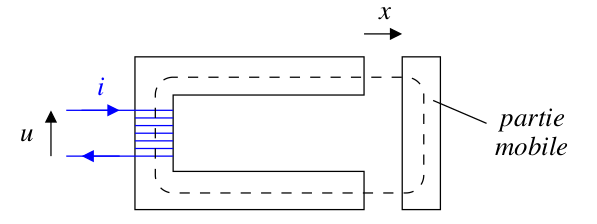
\includegraphics[width=.5\linewidth]{./figures/ContacteurElectromagnetique.png}
    \caption{Contacteur électromagnétique}
\end{figure} 

On considère le matériau  ferromagnétique comme linéaire $\mu_r\ll 1$. Il canalise les lignes de champ magnétique (on peut montrer une simulation PSI Dunod (2020)). On supposera aussi que la section du noyau est petite de façon à ce que $\vec{B}$ et \vec{H} soient uniformes dans une section droite du fer. On note $l$ la longueur moyenne en l'absence de l'entrefer. Si $x$ est suffisamment petit devant $\sqrt{Section}$, le tube de champ magnétique est de section constante dans l'entrefer.

\subsection*{1.2. Énergie magnétique emmagasinée}
\begin{enumerate}
    \item Théorême d'Ampère);

Application du théorême d'Ampère (dans l'ARQS) sur le contour en pointillé: 
\begin{equation}
	H_{fer}\times l + H_{entrefer}\times 2x = Ni
\end{equation}
	\item Conservation du flux du champ magnétique;
	
\begin{equation}
	B_{fer}=B_{entrefer}=B
\end{equation}

    \item Expression de \vec{B} en fonction de l'intensité;

$B_{entrefer}=\mu_0 H_{entrefer}$ et $B_{fer} = \mu_0\mu_rH_{fer}$ En combinant les différentes relations, on en déduit: 
\begin{equation}
	\dfrac{Bl}{\mu_0\mu_r}+\dfrac{B2x}{\mu_0}=Ni\ \rightarrow B = \dfrac{\mu_0Ni}{2x+l/\mu_r}
\end{equation}

    \item Induction propre $\Phi=Li$ à partir du flux dans le bobinage $\Phi=NBS$.

On en déduit : $\Phi = \dfrac{\mu_0N^2S}{2x+l/\mu_r}i$ puis l'expression de $L$.
\begin{equation}
	L(x)=\dfrac{\mu_0N^2S}{2x+l/\mu_r}
\end{equation}
On remarque que dans un circuit magnétique linéaire déformable, l'inductance dépend de la position de la partie mobile.

    \item Énergie magnétique emmagasinée.
\end{enumerate}
\begin{equation}
	E_m = \dfrac{1}{2}L(x)i^2 = \dfrac{1}{2}\dfrac{\mu_0N^2S}{2x+l/\mu_r}i^2.
\end{equation}

Remarque: On peut retrouver ce résultat en utilisant l'expression de l'énergie magnétique volumique : $u_m=B^2/(2\mu_0\mu_r)$ dans un matériau LHI.

\subsection*{1.3. Force électromagnétique (PSI Tec $\&$ Doc 2014)}
On considère l'ensemble constitué par la bobine, les ferromagnétiques et l'entrefer. On suppose qu’un opérateur extérieur déplace le barreau en exerçant la force $\vec{F}_{op}=F_{op}\vec{u}_x$, la bobine
étant traversée par un courant i et soumise à la tension u.

\begin{figure}[ht]
	\centering
	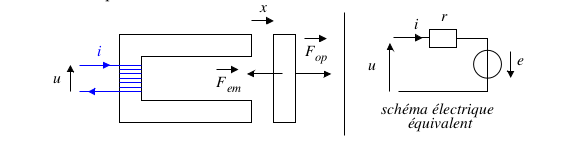
\includegraphics[width=.5\linewidth]{./figures/ForceElectromagnetique.png}
	\caption{Schéma équivalent}
\end{figure}

\subsubsection*{1.3.1. Équation électrique:}
\begin{equation}
	u = ri -e = ri +\dfrac{d\Phi}{dt} \label{eq:eq1CElectromeca}
\end{equation}

\subsubsection*{1.3.2. Premier principe: }
Pendant $dt$, le système reçoit une énergie électrique ($uidt$) et une énergie mécanique $F_{op}dx$ sous forme de travail de la force extérieur qui s'applique sur le bloc en translation. Une partie de l'énergie est dissipée par effet Joule ($Ri^2dt$).
\begin{equation}
	d(E_m+E_c) = \delta W + \delta Q = (uidt+F_{op}dx)-ri^2dt
\end{equation}

Avec l'équation \eqref{eq:eq1CElectromeca} on obtient : 
\begin{equation}
	d(E_m+E_c) = id \Phi+F_{op}dx \label{eq:eq2CElectromeca}
\end{equation}

\subsubsection*{1.3.3. Théorême de l'énergie cinétique (appliqué à la partie mobile)}
\begin{equation}
	dE_c=F_{op}dx+F_{m}dx \label{eq:eq3CElectromeca}
\end{equation}

On compare les équations \eqref{eq:eq2CElectromeca} et \eqref{eq:eq3CElectromeca}, ce qui donne: 
\begin{equation}
	dE_m = id\Phi-F_{m}dx \rightarrow F_{m}dx = id(Li)-d(\dfrac{1}{2}Li^2) \label{eq:eq4CElectromeca}
\end{equation}

Si on développe on trouve : $F_{m}= \dfrac{1}{2}i^2\dfrac{dL}{dx}$ soit:
\begin{equation}
	F_{m} = -\dfrac{\mu_0N^2Si^2}{\left(l/\mu_r+2x\right)^2}
\end{equation}

Si on prend pour valeur $\mu_r=2000$, $N = 500$, $l=50~\rm cm$, $S=16~\rm cm^2$ avec un courant sinusoïdal à $50$ Hz et d'amplitude 50 mA. On trouve $F = 10$ N. On peut lever une masse de 1 kg avec ce dispositif. 

\begin{Resultat}{Il faut noter que :}
	\begin{itemize}
		\item $F_{m}\propto i^2$, c'est une force de rappel quelque soit le signe de $i$ et est nulle en moyenne dans le temps pour une excitation sinusoïdale.
		\item Ce type de dispositif peut servir de contacteur électromagnétique permettant de commander la fermeture et l'ouverture d'un circuit électrique via le déplacement de la partie mobile, qui en l'absence de courant dans la bobine, est ramenée à sa position initiale par l'intermédiaire d'un ressort.
		(\textbf{Discussion et ordre de grandeur} dans le Physique Chimie en PSI/PSI*, chez ellipses par Pascal Olive)
	\end{itemize}
\end{Resultat}

\subsection*{1.4. Généralisation}
La méthode que l'on a appliqué sera toujours la même (Ampère, conservation du flux, inductance propre, énergie emmagasinée, bilan énergétique global). On peut généraliser l'expression de la Force à partir de l'équation \eqref{eq:eq4CElectromeca} tel que : 
\begin{equation}
    F=\left(\dfrac{\partial E}{\partial x}\right)_\Phi
\end{equation}
Pour un contacteur en rotation autour d'un axe fixe $Oz$ repéré par un angle $\theta$, il suffit de changer les travaux extérieurs $\vec{F}_{op}$ et électromagnétique $F_{em}$ en $\Gamma_{op}d\theta$ et $\Gamma_{em}d\theta$ où les $\Gamma$ sont les moments des actions s'exerçant sur le contacteur. 
\begin{equation}
 \Gamma = \left(\dfrac{\partial E}{\partial\theta}\right)_\Phi
\end{equation}



On peut maintenant traité les différents types de moteur. Au programme de PSI ils traient les moteurs synchrones puis à courant continu. La manipulation porte sur un moteur à courant continu donc je choisis de commencer par un moteur à courant continu. On garde néanmoins le moteur synchrone sous le coude pour une troisième partie si le temps le permet (j'en doute) ou pour une ouverture.


\section*{2. Machine à courant continu}
On a vu en première année de PTSI le principe d'action d'un champ magnétique tournant sur un moment magnétique. On réalise la mise en pratique d'un moteur.\medskip

Les machines à courant continu font partie des convertisseurs électro-magnéto-mécanique réversibles. Elles sont utilisées massivement dans toutes les gammes de puissance du fait de la simplicité de leur commande de vitesse.

\subsection*{2.1. Structure}

Les élements qui constituent une machine à courant continu sont: 
\begin{itemize}
	\item Une partie fixe: \textbf{le stator}. Ferro. aimantation permanente ou bobinage parcouru par un courant continu $i_e$. présenté sur le schéma avec une paire de pôle (N et S). Le stator crée un champ magnétique stationnaire $\vec{B}_s$ canalisé par le ferro. Le champ statorique est radial dans l'entrefer.
	
	\item une partie mobile: \textbf{le rotor}. Tourne autour de l'axe $Oz$, ferromagnétique. Encoches incrustées dans le rotor dans lesquelles se logent des conducteurs appelés \og{}brins\fg{}. Ces conducteurs sont disposés en spires bobinées sur le rotor. Les spires sont en série et sont parcourues par le même courant $i$. Le rotor est le siège d'induction de Lorentz.
	
	\item L'organisation des courants rotoriques doit être agencée afin de produire un axe polaire fixe, dirigé de préférence selon $Oy$ pour que le couple soit maximal. Cette propriété est vérifiée si la répartition des courants admet, malgré la rotation du rotor, un plan d'antisymétrie ($Oyz$). Il faut aménager un dispositif qui permet d'imposer un sens de circulation du courant pour la part du bobinage située d'un côté de ce plan et d'inverser ce sens pour celle située de l'autre côté. Ce dispositif se nomme le \textbf{collecteur}. Les spires sont connectées au circuit extérieur par l'intermédiaire des lames du collecteur sur lesquelles frottent les balais. On explique plus en détail le fonctionnement dans la section suivante !
\end{itemize}
\begin{figure}[ht]
	\centering
	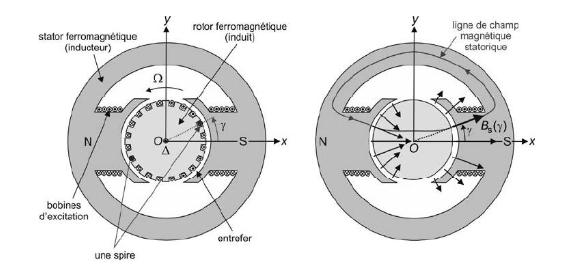
\includegraphics[width=.5\linewidth]{./figures/MCC.png}
	\caption{Schéma d'une machine à courant continu (MCC). Physique Chimie PSI P.Olive, p721. On peut aussi rajouter la simulation des lignes de champ présente dans le Dunod de PSI.}
\end{figure}

\subsection*{2.2. Rôle du collecteur}

Le circuit induit (rotor) est alimenté par le courant continu $i$ qui entre dans le circuit par le pôle + de l'alimentation externe. Une des spires est repérée par la position $\theta$. La connexion de cette spire au circuit d'alimentation montre que si cette connexion reste fixe, le sens de circulation du courant pour la partie de la spire située à gauche du plan $Oyz$ s'inverserait périodiquement en fonction de $\theta$ avec une période de $\pi$.Pour éviter ce changement de sens, on connecte les spires du rotor à l'alimentation par l'intermédiaire d'un collecteur, fixé au sommet du rotor qui permet de raccorder, selon la position de la spire, les bornes de l'alimentation à des extrémités différentes de la spire.\medskip
\begin{figure}[ht]
	\centering
	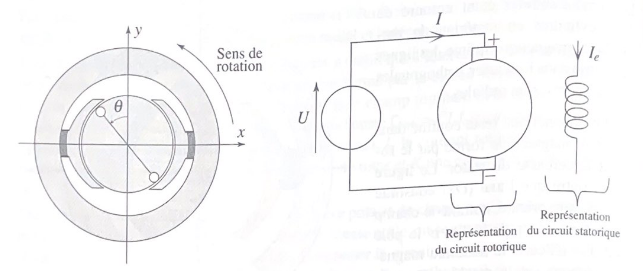
\includegraphics[width=.5\linewidth]{./figures/collecteur1.png}
	\caption{Dunod Psi p 784}
\end{figure}
Le collecteur comporte un ensemble de lames conductrices, électriquement isolées entre elles, situées en tête du rotor. Leur nombre dépend du nombre de spires. L'ensemble de ces lames sont positionnées sur un cylindre posé sur le rotor. Elles tournent donc à la même vitesse que le rotor. Lorsqu'il n'y a qu'une seule spire, le collecteur est composé de deux lames uniquement.

\begin{figure}[ht]
	\centering
	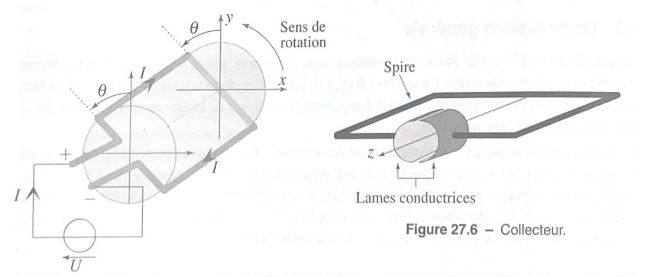
\includegraphics[width=.5\linewidth]{./figures/collecteur2.png}
	\caption{Dunod Psi p 784}
\end{figure}

Le contact entre les lames et le générateur qui alimente le circuit est assuré par deux patins conducteurs fixes (liés au stator), glissant sur les lames du collecteur qui se nomment balais. Lorsque le collecteur tourne avec le rotor, les balais sont au contact de lames différentes. 

\begin{figure}[ht]
	\centering
	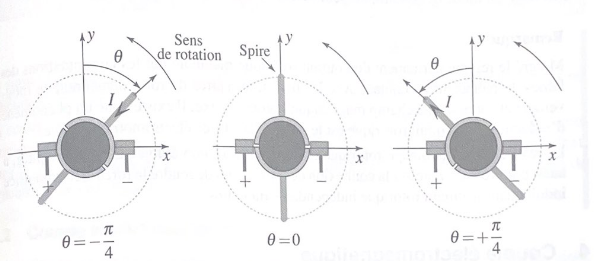
\includegraphics[width=.5\linewidth]{./figures/collecteur3.png}
	\caption{Dunod Psi p 784}
\end{figure}

Pour une seule spire, la direction de l'axe polaire oscille au cours de la rotation du rotor entre $-\pi/2$ et $\pi/2$. Cette oscillation est éliminer dès lors que l'on met un grand nombre de spires. On maintient ainsi la répartition des courants admettant le plan ($Oyz$) comme plan d'antisymétrie. Le champ magnétique est permanent et admet $(Oy)$ comme axe polaire orthogonal à l'axe polaire du stator. Son sens dépend du signe de l'intensité $i$ et du mode de fonctionnement moteur ou générateur de la machine.


\subsection*{2.3. Aproche théorique (Jolidon p 204)}

\subsubsection*{Établissement des équations électromécaniques}

La forme du circuit magnétique cinstitué par le stator et le rotor permet d'établir dans l'entrefer un champ radial. On considère une spire rotorique de hauteur $l$ selon $Oz$ et de largeur $a$, on note I le courant y circulant qui parcourt le segment en $x>0$ selon les $z$ croissants. Le rotor est plongé dans le champ magnétique statorique, chaque segment de spire est parcouru par le courant $I$ subit une force de Laplace:


\begin{equation}
	 d\vec{F}_L =  Idz\vec{e_z}\wedge B\vec{er} = IBdz\vec{e}_\theta
\end{equation}

Cette force est égale à celle s'exerçant sur un point de la spire parallèle à l'axe Oz. Elle génère un couple sur le rotor appelé couple de Laplace. Calculons ce couple.

\begin{figure}[ht]
	\centering
	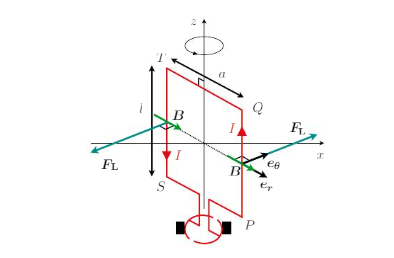
\includegraphics[width=.5\linewidth]{./figures/SchemaPrincipe.png}
	\caption{Schéma de principe extrait du Jolidon}
\end{figure}

\subsubsection*{Couple}

le couple s'obtient en ajoutant le moment subit par les deux branches de la spires soumisent à la force de Laplace:

\begin{equation}
	\mathcal{M} = \int_{M\in[TS]}\vec{OM}\wedge\vec{F_L}(M)+\int_{M\in[PQ]}\vec{OM^\prime}\wedge\vec{F_L}(M^\prime)=IalB\vec{e}_z
\end{equation}

Comme le rotor est constitué de $N$ spires smeblables à celle que nous venons de considérer, on obtient : 

\begin{equation}
	\mathcal{M}_{rotor} = N\mathcal{M} = NialB\vec{e}_z
\end{equation}

Le couple est donc proportionnel au nombre de spires N d'où l'intérêt d'avoir le plus de spires possibles au rotor.\medskip

Le rotor est solidaire d'un arbre de tranmission sur lequel on place une charge à entraîner. Le rotor lui applique un couple $\Gamma$. Discuter du sogne de $\Gamma$ en suivant le Jolidon, permet de décrire le montage expérimental. On établit l'équation mécanique en supposant le référentiel galiléen , théorême du moment cinétique: 

\begin{equation}
	J\dfrac{d\omega}{dt}=-\Gamma-\Gamma_r+NalBI
\end{equation}

On établit l'équation électrique en utilisant la loi des mailles:

\begin{equation}
	U = RI+L\dfrac{dI}{dt}-e_{\rm ext}
\end{equation}

En combinant les équations que l'on a décrit on parvient à un système d'équations:

\begin{equation}
	\left\{
		\begin{array}{cc}
		\Phi\omega & = U-RI-L\dfrac{dI}{dt}\\
		\Gamma & = \Phi I-\Gamma_r-J\dfrac{d\omega}{dt}.
	\end{array}
	\right.
\end{equation}

On a deux équations reliant les quatre variables du quadripôle. En fixant deux d'entre elles on peut déterminer entièrement les variables de fonction du système.

\subsection*{2.4. Caractéristique de fonctionnement}

\subsubsection*{2.4.1. Couple et vitesse de rotation}

En régime permanent de fonctionnement, c'est à dire à $U, I, \Gamma$ et $\omega$ constants le système se réduit à : 

\begin{equation}
	\left\{
		\begin{array}{cc}
		\Phi\omega & = U-RI\\
		\Gamma & = \Phi I-\Gamma_r.
	\end{array}
	\right.
\end{equation}


On voit que les couples de variables mis en jeu sont ($\omega, U$) et ($\Gamma, I$). Le couple est proportionnel à l’intensité i du courant qui circule dans le rotor ($\Gamma = k\Phi$ dans le poly de Phillipe) alors que la vitesse de rotation est pilotée par la tension. Pour un rotor idéal sans pertes joules $R=0$, $\Gamma_r=0$ on aurait même proportionnalité entre $\omega$ et $U$ et $\Gamma$ et $I$.\medskip


Si $i>0$, $\Gamma>0$ la machine fonctionnne en moteur. Si $i<0$ $\Gamma<0$ la machine fonctionne en génératrice.

\subsubsection*{2.4.2. Mesure expérimentale sur un banc d'essai (Poyl TP rennes)}
Poly Phillipe Moteurs - MCC
Réaliser en préparation la mesure de la résistance d'induit pour le moteur et pour la génératrice. On mesure d'abord dans une étude à vide le $\Phi$ dans le moteur avec la génératrice en traçant $E=f(\omega)$
Deuxiemement : étude de charge. On mesure le couple fourni pour une intensité et on trace $\Gamma=f(i)$. Mesure du couple avec une webcam et imageJ. 


\subsection*{2.5. Point de fonctionnement}

La donnée du quadruplet ($U,I, \omega, \Gamma$) est appelée \textbf{point de fonctionnement}  de la machine: il faut donc deux équations supplémentaires pour en déterminer un. Il s'agit de la caractéristique de l'alimentation électrique du rotor généralement de la forme $U = E^\prime-R^\prime I$ ainsi que la caractéristique $\Gamma_c$ de la charge à entraîner. En pratique ces deux nouvelles équations fixent les valeurs de $I$ et $\omega$ vérifiant le système. On peut montrer la caractéristique pour le MCC du Jolidon.

\begin{figure}[ht]
	\centering
  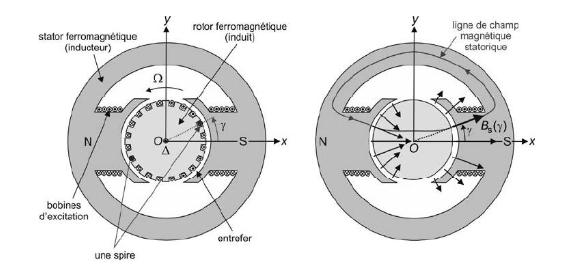
\includegraphics[width=.5\linewidth]{./figures/MCC.png}
	\caption{Caractéristique MCC, extrait du Jolidon}
\end{figure}


\subsection*{2.6. Puissance et rendement (Jolidon)}

Quelque soit son régime de fonctionnement, la MCC consomme de l'énergie dans le stator, en régime moteur, le rotor consomme également une Puissance électrique. Et l'ensemble fournit à la charge mécanique une puissance utile $\Gamma\omega$




\begin{equation}
	\eta_{MCC} = \dfrac{P_{meca}}{P_{elec, stator}+P_{elec,rotor}}
=\dfrac{\Gamma\omega}{UI+U_sI_s}\end{equation}


Le bilan de puissance est déterminé par le système d'equation donné précedemment il suffit de multiplier la premiere equation par I et et $\omega$la deuxieme: 


\begin{equation}
	UI-\Gamma\omega = RI^2+\Gamma_r\omega
\end{equation}

La puissance est dissipe au niveau du rotor, soit par effet joule soit par les pertes mécaniques ($\Gamma_r$). 

Fonctionnement en moteur si $UI>0$ ne donne pas intégrallement la puissance utile $\Gamma\omega>0$ à cause des pertes Joules, mécaniques ainsi que des pertes fer (que l'on a négligé). Fonctionnement en génératrice.

On décrit en suivant le jolidon les différnts types de pertes.

\begin{figure}[ht]
	\centering
	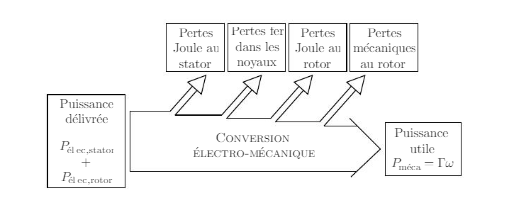
\includegraphics[width=1\linewidth]{./figures/BillanPuissance.png}
	\caption{Bilan de Puissance, extrait jolidon}
\end{figure}

% \section{Machine synchrone}
% On a vu en première année de PTSI le principe d'action d'un champ magnétique tournant sur un moment magnétique. On réalise la mise en pratique d'un moteur.

% \subsection{Structure}
% Dunod PSI 2020 p732-733 et Tec $\&$ Doc 2014 p644, COurs Naval
% La machine synchrone est un exemple de convertisseur électromagnétique réversible, fonctionnant en moteur ou en générateur. Utilisés dans la production d'énergie électrique sous forme de courant alternatif ou bien dans les utilisations de moindre puissance plus courantes comme les véhicules automobiles (Moteur de traction très performant).
% \begin{figure}[ht]
% 	\centering
% 	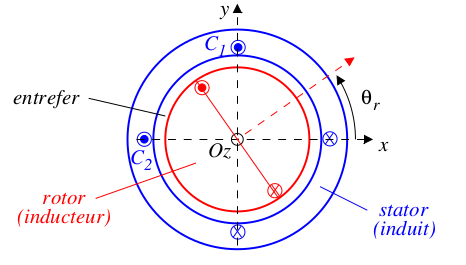
\includegraphics[width=.5\textwidth]{StructureMachinesynchrone.png}
% 	\caption{Schéma cours Naval}
% \end{figure}

% Le matériau constituant le stator (fixe) et le rotor (mobile) est un matériau magnétique linéaire de perméabilité relative infinie. L'épaisseur de l'entrefer est constante. Les deux circuits bobinés sur le stator sont parcourus par un courant sinusoïdal. Le circuit bobiné sur le rotor est parcouru  par un courant permanent. On parle de machine à excitation séparée. L'ensemble du dispositif est de longueur $L$. On cherche à déterminer \vec{B} dans l'entrefer pour en déduire l'énergie magnétique afin de calculer le couple électromagnétique.

% \subsubsection{Stator}
% Partie fixe, alimentés par deux circuits orthogonaux. La machine synchrone est ainsi dite diphasée.
% Champ magnétique tournant avec deux courants sinusoïdaux déphasés de $\pi/2$, voir schéma. (Dunod 2021 PCSI p 877)

% \subsubsection{Rotor}
% Partie ferro tournante, forme variable suivant les applications, rotor à pôle lisses pour de fortes vitesses (entrefer uniforme) cas de l'étude ici.
% Moment magnétique crée avec une spire parcourue par un courant constant.(PCSI 2021 p863 )

% \subsection{Champ dans l'entrefer}

% \subsubsection{Champ crée par une spire}

% Dunod PSI, ligne de champ + contour d'Ampère à dessiner au tableau ou sur transparents. On écrit le théorême d'Ampère, on exprime la circulation dans le Ferro et dans l'entrefer puis comme $\mu_r\ll 1$, on néglige le champ dans le ferro et on en déduit l'expression du champ dans l'entrefer en fonction del'intensité parcourant le fil. Montrer l'allure du champ pour une spire à l'aide d'un programme python ?

% \subsubsection{Répartition spatiale}

% Le champ obtenu avec une seule spire a un défaut majeur : il est discontinu dans l'espace. On cherche à obtenir une répartition angulaire sinusoïdale du champ dans l'entrefer. Si on ajoute d'autres spires avec une répartition spatiale bien choisie, on peut s'approcher d'un champ sinusoïdal (Python ?).

% \subsubsection{Création du champ statorique}
% Il s’agit maintenant de générer à l’aide des deux phases du stator le champ magnétique tournant qui va entraîner le rotor (Cf. principe du moteur synchrone). Deuxième jeu de spires déphasé de $\pi/2$ Calcul dans le Dunod PSI 2020 p 738. On obtient une onde magnétique progressive harmonique qui se propage dans le sens des $\theta$ croissants à la vitesse angulaire $\omega$ ($cos(\theta-\omega t) = f(x-ct)$):
% \begin{equation}
% B_S(\theta,t)=K_SI_S\cos(\theta-\omega t)\vec{u_r}(M).
% \end{equation}


% \subsubsection{Champ rotorique}
% Le rotor tourne en plus d'être parcouru par un courant $i_r$. Sa rotation est repérée par l'angle $\alpha_r$

% Champ magnétique généré par le rotor, rendu spatialement sinusoïdal par la même méthode que pour le champ statorique. $\vec{B}_R(\theta,t)=K_RI_R\cos(\theta-\alpha_r)\vec{u_r}(M)$


% \subsection{Bilan énergétique}

% \subsubsection{Énergie électromagnétique}
% Calcul de l'énergie emmagasinée, DUNOD PSI

% \subsubsection{Couple électromagnétique}
% On reprend la formule donnée dans la première partie et on dérive pour trouver l'expression du couple.
% \begin{equation}
% \Gamma_{em} = \Gamma_{max}\sin{\alpha}.
% \end{equation}
% \begin{Resultat}{Conditions de synchronisme}
% 	La machine synchrone ne développe de couple que si le rotor et le champ glissant statorique tournent à la même vitesse angulaire, ce qui constitue la condition de synchronisme.
% \end{Resultat}


% \subsection{Point de fonctionnement}

% Tracer la sinusoide (Dunod) et commenter.


\section*{Conclusion}

Recap + Interet du moteur à courant continu +machine synchrone

\clearpage

\section*{Leçon 10: Induction électromagnétique}

\hrulefill\\

\noindent\underline{\textbf{Niveau:}}
\begin{itemize}
  \item Licence 3 
\end{itemize}
\underline{\textbf{Pr{\'e}-requis: }}

\begin{itemize}  
\item Electromag 
\item equations de maxwell
\item ARQS
\item mecanique
\end{itemize}
\underline{\textbf{Bibliographie:}}

\begin{itemize}
  \item Dunod PC
  \item Garing
  \item Perez
  \item Ellipse PC 2009 chap induction electromagnetique de Lorentz
\end{itemize}
\hrulefill

\section* {Introduction}

Nous allons voir dans cette leçon que les phénomènes d'induction sont contenus dans les équations de Maxwell et dans la force de Lorentz qu'on a déjà vu. Ils nécessitent qu'on s'y attarde du point de vue des conséquences pratiques qu'ils mettent en exergue. Dans toute la leçon, nous travaillerons dans le cadre de l'ARQS magnétique (i.e. qu'on néglige le courant de déplacement $\mathbf{j_D}=\epsilon_0\dfrac{\partial \mathbf{E}}{\partial t}$ dans les équations de Maxwell).\\
  
  Historiquement : Oersted (1820): courants éléctriques induisent $\mathbf B$. Faraday (1831): Variations de $\mathbf B$ qui induisent des courants électriques. 

  \section*{1. Phénoménologie de l'induction}

  \subsection*{1.1. Mise en évidence expérimentale}



 On prend une bobine en circuit ouvert. On mesure le courant qui passe au travers de la bobine lorsqu'on approche un aimant de la bobine.  L'expérience est décrite dans le dunod de pcsi.

  \textcolor{blue}{Expérience qualitative 1:} Approche un aimant et éloigne un aimant droit d'une bobine fixe branchée à un oscilloscope : apparition d'une tension. Même observation avec déplacement de la bobine dans aimant fixe. Amplitude de l'intensité proportionnelle à la vitesse de variation de $\mathbf B$. De plus, on voit que dans un sens on a une fem positive et dans l'autre une fem négative. Permet de connaitre le pole Nord ou le pole Sud d'un aimant par exemple.


  \begin{definition}{Définition phénoménologique - Induction}
    apparition d'une f.e.m et, s'ils peuvent s'écouler, de courants, dans un conducteur mobile placé d'un champ magnétique variable
  \end{definition}

  \textbf{Deux cas particuliers:} \begin{itemize}
    \item Dans le cas où on a un circuit fixe et un champ variable, on parlera d'induction de Neumann,
    \item Dans le cas où on a un circuit déformable ou mobile dans un champ magnétique stationnaire, on parlera d'induction de Lorentz
\end{itemize}

Ces expériences mettent en évidence le phénomène d'inducion électromagnétique qui se manifeste par l'apparition d'un courant dans un circuit fermé sans qu'il y ait de générateur à l'intérieur dans le circuit. 

\subsection*{1.2. Lois de l'induction (Faraday et Lenz)}

L'équation régissant le phénomène d'induction est la loi de Faraday. On considère une spire plane de forme quelconque placée dans un champ magnétique uniforme $\vec{B}$. On suppose un sens positif conventionnel pour le courant circulant dnas la spire. Définition du flux magnétique traversant la spire: 

\begin{equation}
    \phi =\iint \vec{B}\cdot d\vec{S}.
\end{equation}

\textbf{Validité :circuits filiformes sinon on ne peut pas définir de flux magnétique}

$\phi$ quantifie la quantité de champ magnétique qui traverse la spire dans le sens du vecteur surface. 
Dans les expériences décrites juste avant, on a fait varier le flux magnétique en déplaçant l'aimant par rapport à la bobine. C'est la variation du flux qui provoque l'appartion du courant dans le circuit de la bobine. En 1831, Faraday en déduit la loi suivante:

\begin{equation}
    e = - \dfrac{d\phi}{dt}
\end{equation}
$e$ est la force électromotrice induite. Unités de $e$ (v) et $\phi$ (Wb ou T.m$^2$)Convention générateur de la f.e.m. : la force électromotrice est dans le même sens que l'intensité.\medskip

\textcolor{blue}{expérience qualitative 2 :} chute d'un aimant dans un conducteur.\\
\textbf{Loi de Lenz :} discussion du signe $-$ dans la loi de Faraday.\\

\textcolor{red}{Transition :}On va voir qu'on peut formaliser l'induction à l'aide d'une approche microscopique. 

\subsection*{1.3. Loi de Lenz}

\textbf{Loi de Lenz:} Les phénomènes d'induction s'opposent par leurs effets aux causes qui leur ont donné naissance. Discuter du signe dans la loi de Faraday. \medskip

\textbf{Transition:} maintenant que l'on a vu les lois pour comprendre les phénomènes de l'induction, on va étudier  les deux causes possibles d'apparition de l'induction.

\section*{2. Théorie de l'induction}

\subsection*{2.1. Définition formelle de la fem}

Voir Tec\&Doc PC p617. La tension électromotrice s'exprime de la manière suivante :
\begin{equation}
    e = \frac{1}{q} \oint_{C} \mathbf{F}(\mathbf{r}, t) \cdot d\mathbf{l}
\end{equation}
où C est un contour orienté et fermé et F une force proportionnelle à la charge. La fem représente donc le quotient de la circulation de cette force le long de ce contour pour la charge.\\ 
En utilisant la force de Lorentz dans un référentiel R du laboratoire supposé galiléen : $\mathbf F = -e(\mathbf{E}+\mathbf{v}_R\wedge \mathbf{B})$, où $\mathbf{v}_R$ est la vitesse des électrons dans ce référentiel, on obtient : 
\begin{equation}
    e = \oint_{C} \mathbf{E} \cdot d \mathbf{l} + \oint_C (\mathbf{B} \land \mathbf{v}_R) \cdot d \mathbf{l}
\end{equation}
On voit que si le circuit de contour $C$ est fixe, $\mathbf{v}_R//\mathbf{dl}$ donc le second terme est nul : c'est l'induction de Neumann.

\subsection*{2.2. Induction de Neumann}

Le champ électrique $\mathbf{E}$ s'écrit de manière générale à partir des potentiels scalaire et vecteur :
\begin{equation}
    \mathbf{E} = - \nabla V - \frac{\partial \mathbf{A}}{\partial t}
\end{equation}
Ce qui implique que ($\mathbf{grad}V$ est à circulation nulle sur un contour fermé):
\begin{equation}
    e = \oint_C \mathbf{E_m}\cdot \mathbf{dl}
\end{equation}
ou $E_m = -\dfrac{\partial \mathbf{A}}{\partial t}$ est appelé \textcolor{green}{le champ électromoteur de Neumann}. On retrouve la loi de Faraday en disant que $\oint_C \mathbf{A}\cdot\mathbf{dl}=\int\int_\Sigma \mathbf{B(t)}\cdot d\mathbf{S}=\phi(t)$.
 


\subsection*{2.3. Induction de Lorentz}

Schéma p626 Tec\&Doc PC/PC*. A voir s'il y a le temps ou alors donner les grandes lignes sur slide.\\
 On se place dans un cadre non relativiste et on prend un circuit filiforme ou le circuit est animé d'une vitesse $\mathbf{v_e}$ et la vitesse des électrons dans le référentiel galiléen du labo est $\mathbf{v}_R= \mathbf{v_r} + \mathbf{v_e}$, avec $\mathbf{v_r} // d\mathbf{l}$. \\
 
 Comme on est en régime stationnaire :    $\mathbf E = - \nabla V$. On en déduit la tension électromotrice :
 \begin{equation}
     e = \oint (\mathbf v_e \land \mathbf B) \cdot d\mathbf{l}
 \end{equation}
 Le terme $\mathbf v_e \land \mathbf B$ se subtitue au champ électromoteur de Neumann.\\
 
 Le produit mixe permet d'écrire : 
 \begin{equation}
     e = \oint (d\mathbf {l} \land \mathbf{v_e}) \cdot d\mathbf{B} 
 \end{equation}
Voir Hprépa p179. Le produit vectoriel $d\mathbf {l} \land \mathbf{v_e}$ a pour norme l'aire balayée $d\mathbf{S_b}$ par l'élément de circuit $\mathbf{dl}$ qui va à la vitesse $\mathbf{v_e}$ pendant dt et donc l'intégral représente le flux de B à travers cette surface. Le champ $\mathbf{B}$ étant à flux conservatif, son flux à travers la surface totale $\Sigma_{tot}$ fermée est nul et donc (attention aux signes ! de Sb en particulier) :
\begin{align}
    \oint_{\Sigma_{tot}}\mathbf{B}\cdot d\mathbf{S} &= -\phi(t+dt) + \phi(t) - \oint_{C}\mathbf{B}\cdot d\mathbf{S_b} \\
    -\frac{d\phi(t)}{dt} &= e(t)
\end{align}
On retrouve bien la loi de Faraday.\\

\textbf{Conclusion orale}: Dans le cas général, on a la somme des deux cas (Neumman et Lorentz). On peut passer d'une vision à une autre par changement de référentiel (exemple avec la première expérience qualitative).

\textcolor{red}{Transition :} Maintenant qu'on a bien tous les outils théoriques pour décrire et comprendre l'induction, on va revenir à un aspect pratique.



\section*{3. Circuit fixe dans un champ magnétique variable}

\subsection*{2.1. Auto-induction}

Coefficient d'auto-induction. On a vu qu'une spire parcourue par un courant $i$ générait un champ magnétique. Ce champ magnétique a un flux à travers la spire que l'on nomme flux propre. Comme le flux est $propto$ B qui est $propto$ i, on peut définir un coefficient appelé inductance propre tel que : $\phi=Li$. Comme dans le Dunod on explique sur une seule spire. Calcul de l'inductance propre d'un solenoïde (Dunod p 906). Bilan d'energie (loi des mailles, calcule de la puissance).

Attention ! Le théorême d'Ampère n'apparait qu'en PC et Biot et Savart est hors programme en prepa.

\subsection*{2.2. Cas de deux bobines en interaction}
On présente un schéma de deux spires l'une dans l'autre. La première est alimentée et génère un champ magnétique qui traverse la deuxième bobine. On définit le coefficient d'induction mutuelle et onécrit le lien entre chaque flux et l'intensité de l'autre bobine.

\subsection*{2.3. Manipulation: Mesure d'une inductance L}

cf poly de Philippe. un L fixe (pas de bobine Leybold), oscilloscope , GBF, cabes bananes, bnc, résistances, multimètres, LCR-mètre, transformateur d'isolement(évite les prob de résistance du GBF),

Circuit RL, mesure du temps caractéristique sur oscilloscope avec le temps de réponse à 63%.Ne pas oublier les résistances de la bobine et des câbles

\subsection*{2.4. Inductance mutuelle}
Dessin spire 1 avec ligne de champ et spire 2 dans champ magnétique créé par spire 1. \\
- Flux créé par spire 1 à travers spire 2: $\phi_{21} = M_{21} i_1$ ; \\
- Flux créé par spire 2 à travers spire 1: $\phi_{12} = M_{12} i_2$ ; \\
- $M_{12} = \oint \oint \frac{\mu_0 d \mathbf{l_1} \cdot d \mathbf{l_2}}{4 \pi r_{12}} = M_{21}$. \\
 Modèle simple de transformateur (schéma sur slide). Secondaire en circuit ouvert $(i_2 = 0)$. Loi des mailles (en complexe) donne: $ M = L_1 \left| \frac{U_2}{e_g} \right|$. 
 
\section*{Conclusion} 
Applications diverses (on a vu bobines et transformateurs). \\
Autres applications (slide) : Haut-parleur, Plaques à induction, Feinage par induction.

\clearpage 

\section*{Leçon 11: Rétroactions et oscillations}

\hrulefill\\

\noindent\underline{\textbf{Niveau:}}
\begin{itemize}
  \item CPGE 
\end{itemize}
\underline{\textbf{Pr{\'e}-requis: }}

\begin{itemize}  
\item Programme de première année
\item Stabilité des système linéaires
\item transformée de Laplace
\end{itemize}
\underline{\textbf{Bibliographie:}}

\begin{itemize}
  \item Dunod PSI/PCSI
  \item poly Jeremy Neveu
  \item Poly de philippe
\end{itemize}
\hrulefill


\section*{Introduction}

On peut réaliser une manipulation introductive à l'aide d'un MCC avec une alimentation et une génératrice avec une charge.On sait qu'à vide, il y a proportionnalité entre la tension appliquée et la rotation du moteur. Si onvarie la charge, la vitesse de rotation varie alors que la fem est constante. Il y a donc un problème. Pour que le système continue à tourner à la même vitesse le système doit avoir l'information de ce qui sort et adapter. En réalisant un système bouclé où l'on compare la valeur en sortie avec la valeur en commande.Dessiner un schéma bloc du principe (E la commande, S la sortie, T la perturbation, K ala régulation, G l'additionneur et B le capeur.) \medskip

\textcolor{blue}{Manip qualitative introductive :} MCC asservi (maquette régulation de vitesse) + Oscilloscope + GBF + N fils bananes + N fils BNC. Prendre l'exemple de l'escalator. Discuter : 
\begin{itemize}
    \item asservissement idéal : vitesse = celle de l'entrée = constante même avec des gens dessus (tension de consigne = tension d'entrée, critère de précision),
    \item réponse rapide lorsqu'il y a une personne qui se met sur le tapis (temps de réponse du système, critère temporel),
    \item réponse ne dépasse pas la vitesse de commande pour ne pas avoir dà coup,
    \item critère d'énergie à fournir, etc.
\end{itemize}
Faire varier les corrections et le cas frottements/pas frottements.\\

Finalement on se retrouve dans la plupart des cas à devoir répondre à un cahier des charges plus où moins strict. La problèmatique de l'asservissement est un des critère du cahier des charges qui fait intervenir une notion importante : la notion de système bouclé. Cette notion peut être défini ailleurs qu'en physique voir Tec\&Doc p65 (économie avec les prix, biologie avec le corps humain) mais on va rester en électronique :).On s'intéresse au point de vue de l'électronique. Les systèmes mécaniques seront traités en SI.

\section*{1. Rétroaction : commande d'un système }

\begin{definition}{Définition 1 - Rétroaction}
  Une rétroaction est la réintroduction du signal de sortie d'un système à l'entrée de ce système.

\end{definition}
\subsection*{1.1. Système bouclé}

Présenté sur slide le schéma du système bouclé. 

On définit :
  \begin{itemize}
      \item la fonction de transfert de la chaîne direct $\underline{A}$ : dans le cas de la manip introductive correspond à l'ensemble correcteurs+amplificateur+suiveur de puissance (voir notice),
      \item la fonction de transfert de la chaîne de retour $\underline{\beta}$ qui dans le cas de la manip introductive était un tachymètre. C'est souvent justement un capteur (photodiode pour asservir la lumière, sonde à effet hall pour le champ, etc),
      \item un comparateur (le plus souvent un soustracteur pour l'asservissement) qui renvoit une erreur $\epsilon = \underline{e}-\underline{\beta}\underline{s}$ est appelé signal d'erreur.
  \end{itemize}
  Le signal d'entrée $e$ et le signal de sortie $s$ sont reliés entre eux par une fonction de transfert. Si le système est ouvert en sortie de la rétroaction, alors on appelle FTBO :
  \begin{equation}
      FTBO = \frac{\underline{r}}{\underline{e}} = \underline{A}\underline{\beta}
  \end{equation}
  Si le système est fermé sur la sortie (un dipôle par exemple), alors on définit la FTBF :
  \begin{equation}
      FTBF = \frac{\underline{s}}{\underline{e}} = \frac{\underline{A}}{1+\underline{A}\underline{\beta}}
  \end{equation}


\subsection*{1.2. Un exemple l'amplificateur non inverseur (Dunod p 47)}

Mettre sur slide le schéma bloc, faire les calculs (bien fait dans le dunod p 46). On suit le Dunod de PCSI ou PSI. On présente le schéma électrique. Cahier des charges. Rétroaction pour assure le régime linéaire. On peut faire des observations expérimentales. Calcul de la fonction de transfert, noté l'impédance d'entrée infinie.\medskip

Stabilité (Dunod p 35 et 38)
On reste dans les mêmes conditions (système 1er ordre). Le système est dit stable si le signal de sortie $s(t)$ reste fini pour un signal d’entrée fini. Pour obtenir un critère de stabilité : réponse du système à un échelon de tension. PWP. Intégration de l’équation différentielle pour arriver au critère : $1 + \beta \mu_0 > 0$.Si la condition de stabilité n’est pas respectée dans le système bouclé, des oscillations peuvent apparaitre : comment les rendre utiles ? Comment les maintenir ? 

\subsection*{1.3. Caractéristiques d'un asservissement}

On peut parler de :
\begin{itemize}
    \item précision : différence entre l'entrée et la sortie en $t\rightarrow\infty$ (erreur statique), ou erreur avec laquelle la sortie suit la consigne imposée au système (erreur dynamique)
    \item rapidité : temps au bout duquel le système atteint son régime permanent (pour lexemple de l'ALI non inverseur, c'était $\tau_{BF}$ donc plus la bande passante est large, plus le système réagit rapidement,
    \item stabilité du système : la réponse reste bornée
\end{itemize}
\textcolor{red}{Propriété :} de manière générale, il ya une compétition entre rapidité et stabilité. Explication avec les mains : plus un système va vite, plus il a de chance de dépasser la consigne, le système va suréagir et l'entraîner encore plus loin.

\section*{2. Critères de stabilité}

Tec\&Doc p75. \textcolor{red}{Critère de stabilité :} Un système bouclé évoluant en régime libre (entrée nulle), au voisinage de son équilibre (sortie nulle) sera dit \textcolor{green}{stable} si l'évolution de la sortie tend spontanément vers l'équilibre $s\rightarrow0$, \textcolor{green}{instable} dans le cas contraire.
\subsection*{2.1. Cas des systèmes d'ordre 1 et 2}
Voir Tec\&Doc p71 ou J. Neveu. Poser l'équation différentielle à la sortie en régime libre (entrée nulle) pour $A=\frac{A_0}{1+jt/\tau_0}$  (fonction de transfert 1er ordre) et $\beta=\beta_0$ (gain simple). La solution générale est 
\begin{equation}
    s(t) = S_0e^{-t/\tau'}
\end{equation}
avec $\tau'=\frac{\tau_0}{1+A_0\beta_0}$. L'appliquer à un ALI en montage non inverseur (au programme PSI) et expliquer pourquoi ce n'est pas stable si on inverse les bornes + et - (devient un comparateur à hystérésis), cela revient à inverser le signe de $\mu_0$.\\
On peut montrer la même chose avec un système d'équation différentielle d'ordre 2 (à voir si redémonstration au tableau ou sur slide). On retient :
\begin{itemize}
    \item les systèmes d'ordre 1 et 2 sont stables si tous les coefficients de l'équation différentielle régissant s(t) sont de même signes
\end{itemize}
\subsection*{2.2. Cas des systèmes bouclés}
Voir J. Neveu. (oscillateurs). Montrer le tableau transformée de Laplace, évolution temporelle du signal. Reprendre la fonction de transfert, établir que si :
\begin{itemize}
    \item $A\beta$ possède des parties réelles négatives alors le système est stable.
    \item $A\beta$ possède des parties réelles nulles alors le système est oscillant.
    \item $A\beta$ possède des parties réelles positives alors le système est instable.
\end{itemize}

\textcolor{red}{Transition :} on va voir justement une application de ces conditions de stabilité en étudiant des systèmes qu'on appelle des oscillateurs. 

\section*{3. Oscillateurs quasi sinusoïdaux}
\begin{definition}
  un oscillateur électronique est un circuit alimenté (actif),
bouclé, dans lequel des instabilités donnent naissance à un signal périodique.
\end{definition}


Intérêts :
\begin{itemize}
  \item généré des signaux T-périodiques de tous types qu’on peut émettre avec des antennes ou générer des ultrasons avec un transducteur adapté;
  \item mesurer le temps (montre = résonnateur à quartz, chronomètre, etc.);
  \item molécule sur une surface vibrante va modifier légèrement sa fréquence de vibration : détecteurs de molécules à des très faibles concentrations. 
\end{itemize}

Il en existe deux types : les quasi-sinusoïdaux et les oscillateurs à relaxation. On va se concentrer d’abord sur les oscillateurs quasi-sinusoïdaux en prenant l’exemple de l’oscillateur à Pont de Wien.

\subsection*{3.1. Définition}

Système bouclé auto-oscillant, pas de signal d'entrée, retour sur la stabilité vue juste avant.

\subsection*{3.2. Oscillateur à pont de Wien}

Constitué d'un amplificateur non inverseur et d'un filtre à bande passante. Schéma électrique sur transparent, schéma bloc au tableau.\medskip

\textbf{Pont de Wien:} Pont diviseur de tension d'où la FT.

\subsection*{3.3. Manipulation}

On présente bien les composants au fur et à mesure de l'explication. On donne les conditions d'auto-oscillation. On écrit le rapport $v/s$ et on arrive à la condition que le produit des deux FT est 1. On a alors deux équations: une pour la partie réelle et une pour la partie imaginaire, d'où une condition sur $\omega$ et une condition sur le gain. On réalise l'oscillateur et on choisit une boîte à décades pour la résistance $R_2$ et on cherche sa valeur pour obtenir les oscillations. On vérifie que l'on obtient bien la condition d'auto-oscillation déterminée précédemment. On peut discuter de l'amplitude et de la pureté spectrale des oscillations.

\section*{Conclusion}

On s'est intéressé à la stabilité des systèmes bouclés permettant de discuter des oscillateurs, mais il existe aussi d'autres propriétés comme la rapidité, la précision. Autres types d'oscillateurs (Quartz)

\clearpage

\section*{Leçon 12: Traitement d'un signal. Étude spectrale}

\hrulefill\\

\noindent\underline{\textbf{Niveau:}}
\begin{itemize}
  \item CPGE 
\end{itemize}
\underline{\textbf{Pr{\'e}-requis: }}

\begin{itemize}  
\item Diagrammes de Bodes
\item Électronique, RC, RLC
\item Fonctions de transf ert
\end{itemize}
\underline{\textbf{Bibliographie:}}

\begin{itemize}
  \item Dunod PC, MP, PTSI;
  \item Jeremie Neveu \textit{Télécommunications};
  \item Tailler \textit{Dictionnaire de physique}
\end{itemize}
\hrulefill


\section*{Introduction}

\textcolor{red}{Accroche : (cf cours Jérémy Neveu) }L'enjeu des communications est de pouvoir envoyer un signal (\textit{i.e.} une information) depuis un émetteur jusqu'à un récepteur afin que celui-ci puisse être d'une part reçu et d'autre part compris.

\begin{definition}{Définition 1 - Signal}
  (ref Taillet p674) Variation temporelle ou spatiale d'une quantité physique mesurable (tension, force, lumière, ...) portant une information.
\end{definition}

\begin{definition}{Définition 2 - Traitement du signal}
  Transformation d'un signal reçu par un récepteur pour en retirer l'information transmise initialement par un émetteur. Ex : si un observateur cherche à analyser les nuages émis par le feu (\textcolor{green}{signal}), il doit se séparer de celle émise par l'environnement (\textcolor{green}{bruit}) par différents moyen (se couvrir les yeux pour se protéger du soleil). \og Se couvrir les yeux \fg~ = filtrage.
\end{definition}


\section*{1. Contenu spectral d'un signal périodique}

\subsection*{1.1. Signal périodique non sinusoïdal}

On suit le dunod de MP. On donne la définition d'un signal périodique et sa décomposition en série de Fourier (sur tranparets). On donne la formule de la somme et le calcul de chacun des termes.\medskip

Un signal $s(t)$ est périodique s'il reprend identiquement la même valeur à intervales de temps égaux: $s(t+T)=s(t)$ où $T$ est la période du signal. Tout signal périodique de fréquence $fs$ de forme quelconque est constitué de la superposition de signaux sinusoïdaux de fréquences multiples de $fs$. Ainsi toute fonction réelle peut s'écrire sous la forme d'une somme infinie de fonctions sinusoïdales: 

\begin{equation}
  s(t)=s_0+\sum \left[a_n\cos{2\pi nf_st} + b_n\sin{2\i n f_st}\right]
\end{equation}
Les coefficients complexes $c_n$ sont sous la forme de :

$$  a_n = \dfrac{2}{T}\int_{0}^T{s(t)cos(2\pi nf_s t)dt}$$

$$  b_n = \dfrac{2}{T}\int_{0}^T{s(t)cos(2\pi nf_s t)dt}$$

Remarques: il faut toutjours étudier la parité de la fonction:
\begin{itemize}
  \item si s est paire, la décomposition ne comporte que des fonctions cosinus $b_n=0$
  \item si s est impaire elle ne comporte que des fonctions sinus $a_n =0$
\end{itemize}
On peut réecrire cette somme en regroupant les termes de même fréquence: 

\begin{equation}
  s(t)=s_0+\sum a_n\cos{2\pi nf_st+\phi_n}
\end{equation}

Cette écriture est très pratique, car elle fait apparaItre l'amplitude et la phase du signal. Le terme constant $a_0$ est la valeur moyenne du signal notée $\langle s(t) \rangle$. Les termes en $n$ sont les harmoniques. $n=1$ correspond au fondamental. On décrit la composante continue, i.e. la moyenne du signal. La composante sinusoïdale du fondamental et les harmoniques.

\subsection*{1.2. Exemple avec un signal créneau}
On donne un exemple à l'aide d'un code python. On prend un signal créneau de période $T=2~\rm ms$, d'amplitude crête à crête $s_{cc}=2~\rm V$. Donc de valeur moyenne $\langle s\rangle = 1$. Ce signal admet un développement en série de Fourier. Avec $f=1/T$ la fréquence du signal. Pour un signal créneau, qui est une fonction impaire. Donc $a_n=0$. On choisit un signal centré en $0$. Donc $s_0 = 0$. Il nous reste qu'à calculer les coefficients $b_n$: 


$$b_n = \dfrac{2}{T}\int_{0}^Ts(t)\sin(n\omega t)dt = \dfrac{4}{T}\int_{0}^{T/2}s(t)\sin{n\omega t}dt = \dfrac{-4}{n\pi}(cos(n\pi)-\cos(0))$$
Deux cas : 
\begin{itemize}
  \item si $n$ est pair $b_n=0$
  \item si $n$ est impair $b_n = \dfrac{4}{n\pi}$
\end{itemize}
On peut alors réecrire le signal $s$ tel que:

\begin{equation}
  s(t) = \dfrac{4}{\pi}\sum \dfrac{1}{2n+1}\sin{(2n+1)\omega t}
\end{equation}

On peut montrer numériquement l'approximation d'un créneau et ou d'un triangle par le développement en série de Fourier, On montre que les hautes fréquences permettent d'approximer les variations rapides de la fonction.  Et montrer que ça ne marche pas pour un bruit blanc.

\subsection*{1.3. Spectre d'un signal périodique}

On s'intéresse à un spectre en amplitude, on trace la valeur de chaque coefficient $a_n$ en fonction de la fréquence $f_n$ de l'harmonique. On peut commencer par présenter le spectre d'un sinus pur, et à côté les spectres du signal triangulaire et créneau.

\subsection*{1.4. Action d'un filtre sur un signal périodique}

On rappelle la définition de la fonction de transfert d'un système linéaire: 

\begin{equation}
  H(j\omega) = \dfrac{s}{e} = \dfrac{S}{E}{\rm e}^{j(\phi_s-\phi_e)}
\end{equation}

Ainsi que les définitions du gain et de la phase  associée à la fonction de transfert.  On peut montrer un diagramme de Bode d'un filtre passe bas comme dans le dunod de ptsi et en déduire l'effet du filtre sur un sinus. Puis sur un  signal périodique comme le signal carré.\medskip

\textbf{Manipulation:} On peut caractériser un filtre par exemple passe bas d'ordre 1. On réalise un filtre passif avec un RC qui donne un gain de 1 avant la coupure. On fait la manipulation avec la boîte à décades pour la résistance. Faire l'analyse en préparation. On prend un point ou deux en direct pour aller vite (sur regressi).\medskip

On superpose le filtre et la décomposition de Fourier du signal et on fait varier la fréquence de coupure du passe bande dans le programme python. On montre sur le filtre d'avant qu'en envoyant un signal carré, il est modifié et que selon la valeur de la résistance du filtre, le signal est modifié.  On compare à ce que l'on a vu en première partie.

\textbf{transition : } Maintenant qu’on a décrit un signal et qu’on sait en retirer des informations, on va voir comment en envoyer un et comment le réceptionner.


\section*{2. Électronique numérique}

\subsection*{2.1. Signal réel, signal numérique}
On décrit le processus d'acquisition d'un signal numérique. Acquisition, valeurs continues contre valeurs discrètes. Une acquisition se déroule en deux phases. On prélève des échantillons du signal qu’on convertit ensuite en données numériques. Le principe de base de l’échantillonnage consiste à utiliser un interrupteur commandé par un signal d’horloge. La quantification conduit par nature à des écarts entre le signal réel et le signal équivalent aux valeurs numériques obtenues à l’issue du processus.


\subsection*{2.2. Quantification du signal}
Entre le signal numérisé est la superposition du signal réel et d'un signal d'erreur lié au processus de quantification. Ce bruit d'erreur parasite le signal réel et empêche de voir les détails les plus fins du signal réel. (voir poly de Philippe sur le traitement du signal)
On peut utiliser le programme python Quantification_filtrage.py. 

\subsection*{2.3. Analyse spectrale}

Transformée de Fourier, critère de Shannon. Démonstration rapide basée sur le Dunod MP/MP*. Montrer le critère de Shannon sur l'oscilloscope. Durée d'acquisition sur la résolution etc. Voir poly de Philippe.

\subsection*{2.4. Mise en pratique}

Lire le complément "pratique de l'analyse spectrale" dans le dunod. À compléter avec le PSI/PSI* qui présente un autre aspect, notamment sur une partie à l'oscilloscope.\textbf{Manipulation:} Diapason avec microphone, FFT à l'oscilloscope, mesure via une carte d'acquisition et latispro. On envoie sur le programme python pour analyse. Attention sur le programme python il peut y avoir un probleme. Il faut cliquer deux fois pour s'assure de la prise en compte de la fréquence d'échantillonage.

\subsection*{2.5. Filtrage numérique}

On écrit la discrétisation du filtre d'après la FT : de H on passe à la relation entre s et e, on remplace $j\omega$ par la dérivation. On en arrive après calcul à une relation de récurrence entre l'entrée et la sortie (Dunod MP). On montre pour la dérivation, on évoque l'intégration à l'oral en montrant que sur le programme python ça marche mieux. On revient sur le programme python quantification_fitrage.textbf

\section*{3. Traitement non-linéaire d'un signal: modulation-démodulation}

On bascule sur le programme de PSI. 
Fil conducteur : radio analogique. Cf cours de Jérémy.
Deux problèmes : 
\begin{itemize}
    \item \textcolor{green}{l'encombrement :} par exemple deux personnes qui parlent en même temps,
    \item dimension des antennes : longueur de l'antenne doit être de l'ordre de la longeur d'onde soit 1500km pour $f=20Hz$ et 1.5km pour $f=20000Hz$ ...
\end{itemize}


\subsection*{3.1. Modulation}

On explique le principe, on montre la modulation d'un point de vue mathématique (p151) en détaillant l'impact sur la fréquence. Montrer le spectre en illustration. \textbf{Réaliser la modulation en amplitude avec un multiplieur poly de philippe telecommunications } 


On souhaite passer à des tailles d'antennes raisonnable de l'ordre du mètre : soit $f=\frac{c}{\lambda}=30$MHz : c'est le principe de la modulation.

\textcolor{green}{Modulation :} Accrocher un signal à transmettre à une porteuse : modulation de la porteuse. Ex : pigeon voyageur (porteuse) pour faire passer une lettre (signal modulant) d'un point A à un point B\\

Pour un signal EM : 
\begin{itemize}
    \item $V_m(t)=A+B\cos(\omega_mt)$ pour la modulation (GBF Agilent à $\frac{\omega_m}{2\pi}=500$~Hz : le message à faire passer)
    \item $V_p(t) = V_0\cos(\omega_pt)$ (BGX Métrix à $\frac{\omega_p}{2\pi}=50$~kHz : le pigeon voyageur)
\end{itemize}

Faire le calcul à la sortie d'un multiplieur. Deux cas particuliers : montrer modulation DBPC ($A\neq0$) et DBPS ($A=0$).

\subsection*{3.2. Démodulation}

Principe de la détection synchrone, il faudrait réaliser une détection synchrone.

Intérêt de la 
\textcolor{red}{Attention :} pour que ça puisse fonctionner, il faut que la porteuse puisse être regénérée (on peut le faire avec une boucle à vérouillage de phase cf cours Jérémy, le mentionner peut-être en conclusion de la partie).\\

\textcolor{blue}{Manip qualitative : démodulation par détection synchrone}. Le TP est bien fait, montrer le signal qu'on module, le signal après multiplication par la porteuse et le signal après le filtre passe-bas.

\subsection*{3.3. Autres types de modulation}

Modulation en fréquence, et démodulaton de phase. 

\section*{Conclusion}

On peut ouvrir sur d'autres formes de filtrage

\clearpage
\section*{Leçon 13: Ondes progressives, ondes stationnaires}

\hrulefill\\

\noindent\underline{\textbf{Niveau:}}
\begin{itemize}
  \item CPGE 
\end{itemize}
\underline{\textbf{Pr{\'e}-requis: }}

\begin{itemize}  
\item Mécanique de première année
\item résolution d'équation différentielles
\item Phénomènes ondulatoire, voc longueur d'onde ...
\end{itemize}
\underline{\textbf{Bibliographie:}}

\begin{itemize}
  \item Dunod PC
  \item Dunod PSI
  \item H prepa Ondes 2 eme année pour les calculs
  \item Garing ondes mécaniques.
  \item BUP Ondes \url{https://bupdoc.udppc.asso.fr/consultation/resultats.php}
\end{itemize}
\hrulefill

\section*{Introduction}

On peut introduire en parlant de la diversité d'ondes que l'on peut trouver.
Ondes électromagnétiques (lumière), ondes mécanique (vagues, acoustiques, corde vibrante). 
On peut montrer la cuve à onde, la corde de melde. Montrer que l'on peut observe une déformation qui se propage de proche en proche dans le milieu continu dans les deux cas. 

\section*{Propagation des ondes}

\subsection*{Définition de phénomènes ondulatoires}

Définition floue à cause de la diversité des phénomènes concernés. On donne la définition sur slide. On met les points importants au tableau: Une onde correspnd à la modification des propriétés physiques d'un milieu matériel ou immatériel engendrée par une action locale qui se répercute/ se propage d'un point à un autre du milieu avec une vitesse finie déterminée par les caractéristiques du milieu. Au passage de l'onde, chaque point du milieu reproduit, avec un décalage temporel et une éventuelle atténuation, la perturbation originelle engendrée par une source fournissant de l'énergie au milieu. La propagation résulte généralement du couplage entre deux champs appelés grandeurs couplées.

\subsection*{Corde vibrante (Dunod, Garing)}

\subsubsection*{Modèle et hypothèses}
On considère une corde de longueur $L$, homogène sans raideur, de masse $m$ donc de masse linéique $\mu_l = m/l$. La corde est tendue par une tension $\vec{T_0}$. On suppose la corde horizontale, ce qui revient à négliger l'effet de pesanteur devant la tension. Faire un schéma montrant ce que l'on observe.\medskip

On s'intéresse aux petits mouvements transversaux, orthogonaux à la direction de propagation. On suppose les perturbations engendrées par le mouvement de la corde, par rapport à son état de repos au premier ordre. 

\subsection*{Mise en équations}

On écrit le bilan des forces sur un élément $dx$ de la corde. On projette selon $x$ et $y$  puis on prend le premier ordre pour la projection suivant $y$. On arrive alors à l'équation de d'Alembert:

\begin{equation}
    \dfrac{\partial^2 y}{\partial t^2} = c^2\dfrac{\partial ^2 y}{\partial x^2}.
\end{equation}

avec $c = \sqrt{\dfrac{T}{\mu}}$. On remarque que nous avons propagation d'une onde, car il y a deux grandeurs couplées. Ici les deux grandeurs couplées sont la composante $\vec{T}$ selon $O_y$ et la vitesse de la corde $v_y = \partial y/\partial t$. En effet si on pose $\vec{F}=-T\sin{\alpha}\approx -T\partial y/\partial x$ on a alors: 
\begin{equation}
    \left\{\begin{array}{ll}
        \dfrac{\partial v_y}{\partial t} &= -\dfrac{1}{\mu}\dfrac{\partial F}{\partial x}\\
        \dfrac{\partial F}{\partial t} &= -T\dfrac{\partial v_y}{\partial x}        
    \end{array}\right.
\end{equation} 

(H-prepa p 32) Une déformation de la corde entraîne l’apparition d’une force qui
peut elle-même entraîner une vitesse de déplacement, etc. Nous retrouvons ici
un couplage semblable à celui qui entraîne la propagation d’une déformation
dans la chaîne de masses couplées par des ressorts.

\subsection*{Généralisation}

On peut insister ici sur la généralité de l'équations de d'Alembert qui régit la propagation des ondes. On démontre l'équation de D'alembert rapidement sur transparents pour l'électromagnétisme. On peut évoquer que dans l'année de PC on pverra d'autres types d'équations de propagation (diélectriques, plasmas, etc).  Noter que la célérité de l'onde dépend des paramètres/ caractéristiques du milieu et de l'onde qui se propage. On peut peut être présenter un tableau qui récapitule les différents cas.

\section*{Solutions générales de l'équation de d'Alembert: ondes progressives}

On reprend le Dunod de PC p 892. 

\subsection*{Ondes progressives}

Onde se propageant avec une vitesse $c$ dans la direction de l'axe $Ox$ et dans le sens positif de cet axe. On montre sur transparents la forme de l'onde qui se propage dans une direction, amplitude. Rapidement (programme de première année). Démonstration que c'est une solution générale (On la trouve dans le PSI p870).

\subsection*{Ondes progressives harmoniques}

(Dunod PSI, PC, Hprepa) Faire appel à la lécon sur le traitement d'un signal. On peut décomposer les solutions de l'équation de d'Alembert en une somme de sinusoïdes (c'est permis par la linéarité de l'équation de d'Alembert). On cherche donc des solutions de la forme:
\begin{equation}
    s(x,t) = s_0 \cos{\omega t-kx+\phi}.
\end{equation}

On peut rappeler la signification des différentes grandeurs associées à l'onde: pulsation $\omega$, vecteur d'onde $\vec{k}=\omega/c$ dans le vide, $\phi$ phase à l'origine, période $T=2\pi/\omega$, fréquence, longueur d'onde. 

\subsection*{Relation de dispersion}

Il faut alors déterminer les caractéristiques propagatives de chaque OPPH. Pour ça il faut établir le lien entre $k$ et $\omega$ appelée relation de dispersion. La déterminer pour d'Alembert, déterminer et déphinir la vitesse de phase (pour une opph la vitesse de phase ne dépend pas de $\omega$ donc non dispersive). On peut évoquer un exemple d'ondes non dispesives, le cas des ondes de surfaces dans la cuve à ondes mais que l'on ne va pas s'intéresser à ce cas. On peut toutefois montre un graphique python pour montrer comment serait modifiée la relation de dispersion dans le cas des ondes de surface ?

\section*{Une autre famille de solutions : ondes stationnaires}

\textbf{Manipulation introductive} La corde de Melde.

Montrer un schéma de la corde de Melde, dire que ça correspond au cas étudié déjà en début de leçon. Faire vibrer la corde à une fréquence permettant de bien voir l'aspect stationnaire sans stroboscope. On rappelle ce qu'est une onde stationnaire. 

Rappeller ce qu'est une onde stationnaire: solution de l'équation de D'Alembert. Elle s'écrit:
\begin{equation}
    s(x,t) = s_0\cos(\omega t-kx)+s_0\cos(\omega t+kx)=2s_0\cos(\omega t)\cos(k x).
\end{equation}

\subsection*{Solution de l'équation de d'Alembert}

On a vu expérimentalement un régime stationnaire, les deux variables (x et t) ne semblent plus couplées, on cherche une solution de la forme: $s(x,t) = f(x)g(t)$. Méthode des variables séparées que l'on obtient deux équations différentielles. On résout le système (Hprepa ou Dunod PSI/PC). On représente graphiquement la solution. On rappelle la notion de mode propre, de ventre et de noeuds à l'aide d'un schéma (Dunod PSI).

\subsection*{Corde de Melde}

On mène le calcul du régime harmonique forcé (si le temps le permet sinon on donne le résultat ou on s'aide de transparents). Évoquer la divergence et donc le fait qu'il faudrait prendre en compte la dissipation énergétique.

\textbf{Manipulation} Poly de Philippe. Mesure de fréquences. On se met à une fréquence proche de la résonance sur l'excitateur et on mesure la fréquence à l'aide du stroboscope. On compte les noeuds, on vérifie que le premier noeud n'est pas trop loin du bout, sinon, on corrige en cohérence avec que l'on observe. On note la fréquence, on connaît la masse, donc la tension, on peut donc calculer $c$, on en déduit $\lambda$. À partir du nombre de noeuds et de la longueur de l'expérience, on remonte au fait qu'entre deux noeuds on trouve $\lambda/2$. En préparation on le fait pour différentes masses. Pour avoir une jeu de donné assez grand.

\subsection*{Ondes stationnaire ou onde propagative}

Faire le lien avec la partie précédente: On avait affirmé que les ondes progressives constituent une base des solutions. Les ondes stationnaires doivent pouvoir s'exprimer en somme d'ondes progressives. Le faire et interpréter l'onde stationnaire comme superposition d'une onde progressive et de son image réfléchie à une extrémité.

\section*{Conclusion}

Conclure sur les deux bases de solutions que l'on a trouvé. La question est laquelle choisir face à un problème ? La réponse : Ça dépend. SI on cherche des modes de résonance on cherche des ondes stationnaires, sinon on cherche des ondes progressives. On peut ouvrir sur les paquets d'onde transmission de l'information, enjeu capital dans notre société.

\clearpage

\section*{Leçon 14: Ondes acoustiques}

\hrulefill\\

\noindent\underline{\textbf{Niveau:}}
\begin{itemize}
  \item CPGE 
\end{itemize}
\underline{\textbf{Pr{\'e}-requis: }}

\begin{itemize}  
\item Thermodynamique
\item Écoulement parfait, diffusion thermique
\item Ondes électromagnétiques dans le vide
\end{itemize}
\underline{\textbf{Bibliographie:}}

\begin{itemize}
  \item Dunod PC/PSI
  \item H-prepa
  \item TD Pass
\end{itemize}
\hrulefill


\section*{Introduction}

Les ondes acoustiques font partie des domaines de la physique que les savants ont étudiés pour expliquer les sens humains. D'abord pour l'aspect musical, puis pour l'aspect ondulatoire. Dans cette leçon nous allons nous attarder à comprendre ce que sont physiquement les ondes acoustiques, et s'attacher à expliquer comment le son se propage et comment on peut le détecter. (On peut differencier ondes acoustique et sonore (20Hz- 20kHz))

Deux points sont importants dans cette description :
  \begin{itemize}
      \item La propagation nécessite un milieu matériel pour avoir lieu : expérience de la cloche sous vide (expérience de Otto von Guericke seconde moitié du XVIIème ou Robert Boyle plus performant) \url{https://www.youtube.com/watch?v=BC9Pod4cnpk},
      \item La propagation est issue d'un couplage entre les variations de pression du fluide et les variations de vitesse des particules.
  \end{itemize}

\section*{1. Équation de propagation d'une onde de pression}

\subsection*{1.1. Approximation acoustique}
On considère un milieu de propagation qui est un fluide parfait où on néglige l'effet de la pesanteur. 
\begin{itemize}
  \item Au repos pression uniforme $P0$;
  \item masse volumique $\mu_0$;
  \item vitesse particulaire nulle
\end{itemize}
L'onde sonore est une perturbation par rapport à cet état d'équilibre. Lorsque l'onde sonore est émise, l'état du fluide est décrit par : 

\begin{itemize}
  \item $P(M,t) = P_0+p_1$ avec $p_1$ est une perturbation infinitésimal de $P_0\gg p_1$
  \item $\mu(M,t) = \mu_0 +\mu_1$
  \item $\vec{v}(M,t) = \vec{v_1}$
\end{itemize}

Les grandeurs $p_1/P_0$, $\mu_1/\mu_0$ seront traités comme des infiniments petits du premier ordre,comme toutes les autres perturbations que pourra engendrer l'onde sonore dans le milieu.

\subsection*{1.2. équations locales}

On écrit comme dans H-prepa p.95 l'équation locale de conservation de la masse, l'équation de Navier-Stokes que l'on simplifie avec les hypothèse énoncées plus haut (fluide parfait,...) on arrive à l'équation d'Euler. On linéarise et on explicite le coefficient de compressibilité. On arrive aux trois équations suivantes:

\begin{equation}
  \left\{\begin{array}{ll}
    \dfrac{\partial \mu}{\partial t}+\rho_0\vec{\nabla}\cdot \vec{v} &= 0\\
    \rho_0\dfrac{\partial \vec{v}}{\partial t} &=-\vec{\nabla}p\\
    \mu &= \rho_0\chi_s p.
  \end{array}\right.
\end{equation}

En éliminant $\mu$ on parvient à deux équations couplées pour la vitesse et la pression. On arrive à l'équation de d'Alembert en dérivant par rapport au temps l'équation sur la pression. Expliciter la célérité du son dans l'air. Faire l'analogie à l'équation de D'Alembert en électromagnétisme, mais attention relevé les différences entre les deux !!

Pour la célérité du son on peut donner des ordres de grandeur (H-prepa) pour les différents types de fluides. 

\textbf{Manipulation : } Mesure de la vitesse du son dans l'air et dans l'eau.

\subsection*{1.3. Effet Doppler (application à la médecine effet doppler carotidien)}

Mesure de vitesse d'un mobile par effet Doppler. On utilise le principe que l'onde sonore se déplace dans l'air à une vitesse constante (cf d'Alembert) Le déplacement de l'objet par rapport à l'onde entraîne un décalage en fréquence entre l'onde émise et l'onde reçue par le récepteur:

\begin{equation}
  \nu^\prime = \nu \dfrac{c-v_{obs}}{c-v_{source}}
\end{equation}

Si on utilise des ultrasons, la différence de fréquence est donnée dans les deux cas par la relation approchée: 

\begin{equation}
  \Delta\nu = |\nu_R-\nu_E|\approx \dfrac{2\nu_E V}{c}
\end{equation}

\section*{2. OPPH}

\subsection*{2.1. Notations complexes}

On repart directement de l'équation de d'Alembert, on montre la relation de dispersion.
Montrer que la vitesse de phase est indépendante de la pulsation. Propagation non dispersive. C'est cool, car on peut donc les utiliser pour les télécommunications. Ondes longitudinales. 

\subsection*{2.2. Notion d'impédance acoustique}

Du système couplé on en déduit la relation $p=\rho_0 c v_1$. On définit l'impédance $Z$ qui quantifie le couplage entre les deux grandeurs.  Donner des ordres de grandeurs. On peut insister sur l'importance de l'impédance, ne dépend que du milieu et permet de connaître la perturbation en $\mu$ en fonction de celle $v$. Elle va nous permettre de traduire le comportement des ondes aux interfaces entre différents milieux. Ce qui nous intéresse ce n'est pas la perturbation en soit mais l'énergie transportée par l'onde acoustique. On peut proposer un exercice d'adaptation d'impédance dans les échographie.  

\subsection*{2.3. Aspect énergétique}

\subsubsection*{2.3.1 Puissance transférée à travers une surface }

On admet les expression de densité d'énergie volumique, on démontre l'équation de continuité :

\begin{equation}
  \dfrac{\partial e}{\partial t}+\vec{\nabla}\cdot\vec{\Pi}=0.
\end{equation}

\subsection*{2.4. Intensité sonore}

Une fois le vecteur de Poynting explicité, on donne la signification de l'intensité sonore à partir du vecteur de Poynting ainsi qu'en décibels.

\section*{3. Production, transmission et détection d'une onde sonore}

\subsection*{3.1. Ondes sphériques}

Ondes sonores à symétrie sphérique produite par une sphère dont le rayon varie. On aprt de l'équation de D'Alembert en sphérique. On montre que l'amplitude de l'onde décroît en $1/r$ et l'intensité en $1/r^2$. On suit le Dunod de PC, jusqu'à trouver l'intensité sonore en décibels en fonction des grandeurs $I=\log\left(\dfrac{a^2\omega^4r_0^4}{2cr^2I_0}\right)$ On peut changer $a$ et $\omega$. hautes fréuences $a grand$. Pour les hautes fréquences $a$ varie beaucoup. mais on peut changer le rayon de la sphère pulsante pour obtenir une cariation d'amplitde $a$ plus faible : Application aux Hauts parleurs présents sur les chaîne Hifi. 

\subsection*{3.2. Réflexion, transmission application à l'échographie médicale: adaptation d'impédance} 

On résoud l'exercice du TD de PASS, on complète avec l'étude documentaire du TOUT en Un de PSI. 2020. 

\section*{Conclusion}

Les ondes acoustiques sont des solutions de l'équation de d'Alembert comme EM. Mais différentes ce sont des ondes longitudinales qui nécessitent d'un milieu pour se propager. Elles sont très importantes pour notre société lié à la palette d'application : télécom, imagerie médicale etc.

\clearpage

\section*{Leçon 15: Propagation guidée des ondes}

\hrulefill\\
\noindent\textbf{\large Niveau:}\medskip

L1/L2\medskip

\noindent\textbf{\large Prérequis:} \medskip 

\begin{itemize}
	\item Propagation des ondes électromagnétiques dans le vide et les milieux conducteurs
	\item Réflexion sur un conducteur parfait
	\item Ondes acoustiques
	\item Fibre optique à saut d’indice
\end{itemize}


\noindent\textbf{\large Références:} \medskip
\begin{itemize}
	\item Cours d’Etienne Thibierge sur les ondes pour la prépa Agreg de Lyon.
	\item BUP 742
	\item Dunod PC
	\item Sujet Agreg 2009/2004
\end{itemize}

\hrulefill\\

\section*{Introduction}

Pour transmettre une onde sphérique (sonore ou électromagnétique) à partir d'une source, on voit qu'il y a un problème car l'amplitude de l'onde varie en $1/r$ et la densité locale d'énergie de l'onde varie en $1/r^2$ par conservation de l'énergie. Si on veut transmettre une information, il faut donc soit une très grande puissance à l'entrée (dangereux et pas spécialement possible techniquement), soit être plus malin et guider l'onde jusqu'au récepteur. On va cependant voir qu'il existe quelques contraintes.
\textcolor{blue}{Expérience qualitative : deux émetteurs piézo avec ou sans tube.}

\section*{1. Propagation guidée d'ondes acoustiques}
\subsection*{1.1. Intérêt du guide d'onde}

\textit{On règle le générateur de salves pour produire 5 à 10 pulses et on observe l'amplitude du signal
transmis Y avec et sans le tube. On doit récupérer un signal plus fort avec le tube (intérêt du guidage)
et constater la présence d’au moins deux trains d’ondes si on augmente la sensibilité de la voie Y}

% \begin{figure}[!ht]
% 	\centering
% 	\includegraphics[width=.5\textwidth]{guidageTPRennes.png}
% 	\caption{Manipulation-gudiage d'une onde acoustique}
% \end{figure}

\textbf{Observations:}
\begin{itemize}
	\item On observe à l'oscilloscope le signal émis par l'émetteur et le signal reçu par le récepteur;
	\item On note l'amplitude du signal émis par rapport au signal reçu par l'émetteur. Signal reçu nettement plus faible que le signal reçu.
	\item On peut vérifier que $c=340~\rm m\cdot s$
	\item Mesurer l'amplitude à deux distances différents (\textit{ex:} $L = 15~\rm cm$ et $L=41~\rm cm$)
	\item Comparer avec la prédiction donnée par la conservation de l'énergie.
	\item Mettre le guide d'onde. Mesurer l'amplitude du signal. Et montrer que l'amplitude est beaucoup plus grande. 
	\item Remarquons l'apparition de signaux supplémentaires derrière le fondamental.
\end{itemize} 

Transition : Le signal de l'onde sonore est transmis avec moins de pertes d'amplitudes grâce au guide d'onde. En revanche pour faire cela, nous avons dû imposer des conditions strictes sur l'onde. Il en résulte un signal plus fort certes mais dispersé.

\subsection*{1.2. Mise en équations}

On se propose de faire l'étude analytique de la propagation d'une onde sonore dans un guide rectangulaire.

\subsubsection*{1.2.1. Approximation des ondes sonores}
Pour réaliser cette étude, nous allons considérer que l'onde acoustique est une petite perturbation par rapport à l'état d'équilibre:
\begin{itemize}
	\item Fluide considéré comme parfait;
	\item La pesanteur est négligée;
	\item $\frac{p_1}{p_0}\ll 1$;

\noindent On peut comparer l'état d'équilibre $P_0= 1~\rm bar = 10^5~\rm Pa$ au seuil de douleur qui est de l'ordre de $20$ Pa, et l'autre limite le seuil minimum de l'audible $2\cdot 10^{-5}$ Pa.
	\item  $\frac{v_1}{c}\ll 1$ avec $c=340~\rm m\cdot s$;
	\item $\frac{\mu_1}{\mu_0}\ll 0$.
\end{itemize}

\subsubsection*{1.2..2 Mise en équation}

\begin{definition}{Définition - Équation de d'Alembert}
	\begin{equation}
		\Delta p_1 -\frac{1}{c^2}\frac{\partial^2 p_1}{\partial t^2}.
	\end{equation}
\end{definition}
La démonstration sera dans les pré-requis. La noter quand même pendant la préparation pour se préparer aux questions éventuelles. Notamment pour les hypothèses que l'on met en jeu pour parvenir au résultat ! 

\subsubsection*{1.2.3. Position du problème}

% \begin{figure}[!ht]
% 	\centering
% 	\includegraphics[width=.3\textwidth]{guideOndeAcoustique.png}
% 	\caption{Schéma du guide Onde acoustique (Agreg 2009)}
% \end{figure}

\begin{itemize}
	\item $a\ll\lambda$ et $b\ll \lambda$.
	\item Les paroies imposent la condition aux limtes tel que $\vec{v}\cdot \vec{n}$
\end{itemize}

\subsection*{1.3. Recherche de l'onde sonore : l'équation de d'Alembert}
On cherche une solution stationnaire à l'équation de propagation des ondes acoustiques appliquée à ce guide d'onde. Pour ce faire on cherche une solution du type:

\begin{equation}
	p_1(x,y,z,t) = F(x)G(y)H(z){\rm e}^{j\omega t}
\end{equation}

On remplace cette expression dans l'équation de d'Alembert et il vient : 

\begin{dmath}
F''(x)G(y)H(z){\rm e}^{j\omega t}+ F(x)G''(y)H(z){\rm e}^{j\omega t} + F(x)G(y)H''(z){\rm e}^{j\omega t}=-\frac{\omega^2}{c^2}F(x)G(y)H(z){\rm e}^{j\omega t}.
\end{dmath}
On divise par $p_1$: 

\[\frac{F''}{F} + \frac{G''}{G} +\frac{H''}{H}=-\frac{\omega^2}{c^2}\]

Étant donné que les variables $x,y$ et $z$ sont indépendantes les unes des autres, alors $\dfrac{F''}{F}$,$\dfrac{G''}{G}$,$\dfrac{H''}{H}$ sont égales à des constantes. Dans ce cas on obtient le système d'équations suivant: 

\begin{equation}
    \left\{
    \begin{array}{ll}
        
	\frac{1}{F(x)}\frac{d^2 F}{dx^2} &=-k_x^2 \\
	\frac{1}{G(y)}\frac{d^2 G}{dy^2} &=-k_y^2 \\
	\frac{1}{H(z)}\frac{d^2 H}{dz^2} &=-k_z^2

\end{array}
    \right.
\end{equation}

avec  $$\dfrac{\omega^2}{c^2}= k_x^2+k_y^2+k_z^2$$
1111
Pour résoudre ces équations nous avons besoin des conditions aux limites qui imposent que $\vec{v}\cdot \vec{n} = 0$. La vitesse est tangente à la paroie, par conséquent $v_x$ et $v_y$ sont nuls et $\partial p/\partial n = 0$  ($\mu_0 c \vec{v_1} = p_1$) soit:

$$F'(x=0)=F'(x=a)= 0~\text{et}~ G'(y=0)=G'(y=a)=0$$


\begin{itemize}
    \item Si $k_x^2<0$ le discriminant est positif et les solutions sont de la forme d'une somme d'exponentielles réelles. Cette solution ne peut pas s'annuler deux fois donc la solution est nulle.
    \item Si $k_x^2$ est positif le discriminant est négatif et donc les solutions de l'équations sont des solutions sous la forme d'une somme de cosinus et de sinus ou d'exponentielles complexes.
\end{itemize}

\begin{equation}
	F(x) = Acos(k_x x) + Bsin(k_x x)
\end{equation}
En vue des conditions aux limites il vient:

\begin{equation}
	F(x) = cos\left(\frac{n\pi}{a}\right) \textrm{ avec } n\in\mathbb{N}
\end{equation}

En suivant le même raisonnement il vient pour G(y):

\begin{equation}
	G(y) = cos\left(\frac{m\pi}{b}\right) \textrm{ avec } m\in\mathbb{N}
\end{equation}

Enfin on écrira $H(z)$ sous la forme : 

\begin{equation}
	H(z) A_{m,n}{\rm e}^{jk_z z}+ B_{m,n}{\rm e}^{-jk_z z}
\end{equation}

avec \[k_z^2 = \frac{\omega^2}{c^2}-k_x^2 - k_y^2\]

On en déduit $p_{m,n}$ tel que : 


\begin{equation}
	p_{m,n} = cos\left(\frac{n\pi}{a}\right)cos\left(\frac{m\pi}{b}\right)\left[A_{m,n}{\rm e}^{j\left(\omega t+ k_z z\right)}+ B_{m,n}{\rm e}^{j\left(\omega t- k_z z\right)}\right]
\end{equation}

Et la solution $p_1$ : 

\begin{equation}
	p_1(x,y,z,t) = \sum_n\sum_m p_{m,n}.
\end{equation}

\subsection*{1.4. Structure des ondes dans les guides d'onde}
\subsubsection*{1.4.1. Relation de dispersion}

À une fréquence donnée $\omega = 2\pi f$ nous trouvons donc plusieurs modes de propagation, caractérisés par $n$. La relation entre $omega, k$ et $n$ est donnée par \textbf{la relation de dispersion}.

\begin{Resultat}{Relation de dispersion}
	\[k_z^2 = \frac{\omega^2}{c^2}-\left(\frac{n\pi}{a}\right)^2-\left(\frac{m\pi}{b}\right)^2\]
	\begin{equation}
		k_z^2 = \frac{\omega^2-\omega_c}{c^2}
	\end{equation}
	ou encore : 
	\begin{equation}
		\frac{1}{\lambda_g^2} = \frac{1}{\lambda^2}-\frac{1}{\lambda_c^2}
	\end{equation}
	Chacun des termes de la relation de dispersion est positif, ce qui contraint les valeurs permises de $n$ pour un $\omega$ donné. Donc une onde de fréquence donnée ne peut se propager que dans un nombre fini de modes.
\end{Resultat}

% \begin{figure}[!ht]
% 	\centering
% 	\includegraphics[width = .5\textwidth]{Relation_dispersion.png}
% 	\caption{Relation de dispersion}
% \end{figure}

Il faut commenter le fait que cette relation de dispersion est très générale. Valable pour les ondes électromagnétiques, notamment cas du guide d'onde rectangulaire. Étudions le cas tel que $m=0$. Exprimer la relation de coupure et la calculer. Place les différentes pulstions de coupure sur le graphique au fur et à mesure.

\subsection*{1.5. Vitesse de phase et de groupe}

\begin{definition}{Définition - Vitesse de phase et de groupe}
	\begin{equation}
		v_{\phi} = \dfrac{\omega}{k_z} = c\dfrac{\omega}{\sqrt{\omega^2-\omega_{n}}}=\dfrac{c}{\sqrt{1-\left(\dfrac{\omega_n}{\omega}\right)^2}}>c
	\end{equation}
	L'information n'est pas contenue dans la pahse c'est l'enveloppe qui code l'information.

	\begin{equation}
		v_{\phi} = \frac{d\omega}{dk_z} = c\frac{\lambda}{\lambda_g}<c
	\end{equation}
\end{definition}

	$k_{z}^2 < \dfrac{\omega^2}{c^2} $ donc $ \lambda_g > \lambda $

% \begin{figure}[!ht]
% 	\centering
% 	\includegraphics[width=.5\textwidth]{vitesse_de_groupe.png}
% 	\caption{Vitesse de groupe en fonction de l'espacement entre les deux plans conducteurs.}
% \end{figure}

\subsubsection*{Cas du guide d'onde circulaire}

Voir poly de Philippe ou BUP 742
\begin{equation}
	k_z^2 = \frac{\omega^2}{c^2}-\left(\frac{\mu_{nm}}{2\pi a}\right)^2
\end{equation}

Pour que l'onde se propage dans ce guide d'onde il faut que $\omega>\omega_c$ soit $\lambda_c>\lambda$:
\[\frac{\pi d}{\mu_{m,n}}>\lambda\]
Ce qui donne \[d>\frac{\mu_{n,m}}{\pi}\lambda\]

Dans le tube le mode supérieur au mode fondamentale est le mode $\mu_{1,1}=1.84$. Ce qui nous donne:
\begin{equation}
	d>0.59\lambda = 5mm
\end{equation} 


\begin{itemize}
	\item tube de diametre 4.5 mm : monomode
	\item tune de 17 mm plusieurs modes sont visibles.
	\item On mesure les différentes vitesses observées et on essaye de les relier aux vitesses calculées pour le guide d'onde circulaire à l'aide du BUP 742
\end{itemize}

% \begin{figure}[!ht]
% 	\centering
% 	\includegraphics[width=.3\textwidth]{munm.png}
% 	\caption{tableau des $\mu_{m,n}$}
% \end{figure}

du coefficient $mu_{n,m}$ on en déduit $\lambda_c$ qui nous permet de calculer $\lambda_g$ et enfin la vitesse correspondante. Pour le tuyau de diamètre $17~\rm mm$ on peut trouver 6 modes différents:
\begin{enumerate}
	\item 02: v= 270 m/s
	\item 11: v= 324.7 m/s
	\item 12: v= 179/5 m/s
	\item 21: v= 297.3 m/s
	\item 31: v= 253.5 m/s
	\item 41: v= 180.5 m/s
\end{enumerate}


\section*{2. Propagation guidée d'une onde électromagnétique}

S'il nous reste du temps on peut parler de la fibre optique à gradient d'indice. Application majeure dans notre société, télécommunications... On explique au moins le principe de guidage de la lumière à l'aide d'un schéma. Si plus de temps disponible j'en doute. On peut parler des modes de porpagation de l'onde électromagnétique.

\subsection*{2.1. Fibre optique à saut d'indice}


On parlera de la fibre à saut d'indice. Pour que le guidage dans le coeur de la fibre soit efficace il ne faut pas que l'amplitude de l'onde soit diminuée par la partie réfractée : on doit se placer dans les conditions de \textbf{réflexion totale} : $n_2>n_1$ et l'angle $\theta$ tel que: $\cos\theta > \frac{n_2}{n_1}$.

\textcolor{green}{Schéma de la fibre optique à saut d'indice à placer ici}

Les angles d'incidence permettant la propagation dans la fibre prennent des valeurs discrètes. Chaque valeur de l'indice $n$ définit \textbf{un mode de propagation} dans la fibre optique.

\subsection*{2.2. Guidge d'une onde électromagnétique}

On pourrait étudier directement le problème précédent à l'aide de l'électromagnétisme mais calculs compliqués.

\subsubsection*{2.2.1. Position du problème}

\begin{enumerate}
	\item On considère que les deux plans conducteurs sont parfaits. Il n'y a pas de perte d'énergie lorsque l'onde se réfléchi sur la paroie (=absence d'onde évansescente).
	\item On suppose que le milieu où se propage l'onde est vide $n=1$.
\end{enumerate}

\begin{definition}{}
	On étudie la propagation d'une onde électromagnétique dans le vide limité par deux plans conducteurs parfaits.
\end{definition}



% \begin{figure}[!ht]
% 	\centering
% 	\begin{tikzpicture}
% 		\draw[-latex] (0,0) -- (0,2);
% 		\draw (-.5, 2.0) node{$x$};
% 		\draw (-.2,1) -- (0,1);
% 		\draw (-.3,1) node{$a$};
% 		\draw (-.2,0)--(0,0);
% 		\draw (-.3,0) node{$0$};
% 		\draw[fill = gray!40] (0,0)--(5,0)--(5,-.2)--(0,-.2)--cycle;
% 		\draw[fill = gray!40] (0,1)--(5,1)--(5,1.2)--(0,1.2)--cycle;
% 		\draw[-latex] (0,0)--(5.5,0);
% 		\draw (6,-.5) node{$z$};
% 		\croix{1}{.5};
% 		\draw (1,.5) circle(.15);
% 		\draw[-latex, red] (1,.5) -- (2,.5);
% 		\draw (2.5,.25) node{$\vec{e}_z$};
% 		\draw (4,2) node{\textcolor{gray}{Conducteurs}};
% 	\end{tikzpicture}
% 	\caption{Schéma du guide d'onde électromagnétique}
% 	\label{fig1}
% \end{figure}

\begin{definition}{Définition - Équation de propagation}
	\begin{equation}
		\Delta\vec{E} - \frac{1}{c^2}\frac{\partial^2E}{\partial t^2} = 0.
	\end{equation}

	valable aussi pour le champ $\vec{B}$
\end{definition}

% \begin{remarque}
	\textbf{Remarque: } Ce démontre à partir des équations de Maxwell en prenant le rotationnel du rotationnel de E. On intervertit les symboles opératoires.
% \end{remarque}


\subsubsection*{2.2.2. Conditions aux limites}


Ces ondes, pour se propager dans le guide, doivent être compatibes avec les conditions aux limites imposées par les relations de passage entre le vide et les conducteurs parfaits.

	\textbf{Relation de passage:}\medskip

	\begin{itemize}
		\item Continuité de la composante normale de $\vec{B}$ (en $x=0$ et en $x=a$)
		\[\vec{B}(x=a)\cdot(-\vec{e_x}) = 0 = \vec{B}(x=0)\cdot(+\vec{e_x})\]
		\item Continuité de la compoasnte tangentielle de $\vec{E}$ (en $x=0$ et en $x=a$)
		\[\vec{E}(x=a)\wedge(-\vec{e_x}) = 0 = \vec{E}(x=0)\wedge(+\vec{e_x})\]
	\end{itemize}

On suppose que l'on a invariance par translation suivant ($Oy$), et donc les champs ne dépendent pas de la variable $y$.

\subsubsection*{2.2.3. Modes Transverses Électriques et Magnétiques}

On peut mettre en évidence deux groupes d'ondes les ondes Transverses Électriques et Magnétiques.

\[\vec{\nabla}\wedge \vec{E} = ...\]

\[\vec{\nabla}\wedge \vec{B} = ...\]

On voit apparaître deux groupes (E_y, Bx, Bz) que l'on appellera le mode transverse électrique TE. Et le groupe (B_y, Ex, E_z) le groupe transverse magnétique. On dit que le champ électrique du groupe TE est transverse à la direction de propagation. 

\subsection*{2.3. Étude d'un mode transverse électrique}

La linérarité des des équations de d'Alembert et les conditions aux limites permettent d'étudier séparément les ondes TE et TM. 
On cherche une solution de l'équation de propagation sous la forme d'une onde progressive qui se propage dans la direction $\vec{e_z}$ sous la forme:

\begin{equation}
	\vec{E}_y = E(x){\rm e}^{j\left(\omega t-k x\right)}\vec{e_y}
\end{equation}

Pour trouver la forme de $E(x)$, on remplace la forme de la solution dans l'équation de propagation. Il vient:

\[\frac{\partial^2 E(x)}{\partial t^2} + \left(\frac{\omega^2}{c^2}-k^2\right)E(x) = 0.\]

On remarque que la nature des solutions de cette équation dépend du signe de $K^2= \frac{\omega^2}{c^2}-k^2$.


\begin{enumerate}
	\item si $K<0$, dans ce cas la solution est de la forme: 
	\[E(z) = \alpha{\rm e}^{Kx}+\beta{\rm e}^{-Kx}\]
	Cette solution ne peut pas s'annuler en $x=0$ et en $x=a$, donc cette solution est nulle.
	\item si $K= 0$, alors la solution est affine:
	\[E(z)=\alpha x + \beta\]
	Même conclusion
	\item si $K>0$, Dans ce cas la solution s'écrit comme suit:
	\[E(z) = \alpha\cos(Kx)+\beta\sin(Kx).\]
\end{enumerate}
	
\noindent Les condition aux limites : $E(x=0)=E(x=a) = 0$, imposent des solutions telles que $A = 0 $ et $Ka=n\pi~n\in \mathbb{N}$. Par conséquent, une solution de l'équation de d'Alembert est: 

\begin{equation}
	\vec{E} = E_{0,n}\sin{\left(\frac{n\pi}{a}x\right)}{\rm e}^{j\left(\omega t-kx\right)}\vec{ey}
\end{equation}

On peut déterminer le champ $\vec{B}$ en calculant: 

\[\vec{\nabla}\wedge \vec{E} = -\frac{\partial B}{\partial t}.\]

On trouve : 
\begin{dmath}
\vec{B} = jE_{0,n}\frac{n\pi}{a}\cos(Kx){\rm e}^{j(\omega t -k x)}\vec{e_x} + \frac{k}{\omega}E_{0,n}\sin(Kx){\rm e}^{j(\omega t-kx)}\vec{e_z} 
\end{dmath}

Les conditions aux limites nous donnent la structure de l'onde. Il n'y a pas que le milieu de propagation qui influe mais aussi les conditions aux bords. 

\subsection*{2.4. Relation de dispersion}

On retrouve la même relation de dispersion que précédemment.

	\textbf{Relation de dispersion:}\medskip

	\begin{equation}
		k^2  = \frac{\omega^2}{c^2}-K^2 = \frac{\omega^2}{c^2} - \left(\frac{n\pi}{a}\right)^2.
	\end{equation}


	TE$_n$ ne peuvent se propager que si \[\omega \geq n \frac{n\pi c}{a}\]

	\noindent Aucune onde de $\omega < \frac{\pi c}{a}$ ne peut se propager.

\textbf{Remarque:}
	le cas où $k^2<0$ correspond au cas des ondes évanescentes.

\subsection*{2.5. Vitessexs de groupe et de phase}

Un paquet d'ondes est constitué du produit d'une onde \textbf{porteuse} modulée par une \textbf{enveloppe}. L'onde porteuse se propage à la \textbf{vitesse de phase}, tandis que l'enveloppe se propage à la \textbf{vitesse de groupe}.\medskip

\textcolor{green}{Schéma porteuse / enveloppe}\medskip


\noindent On peut réecrire la relation de dispersion tel que: 
\[\frac{\omega^2}{c^2}-k^2=\frac{\omega_n}{c^2}\]
De sorte que: 
\begin{equation}
	k^2 = \frac{\omega^2-\omega_n^2}{c^2}
\end{equation}


	\noindent\textbf{Vitesse de phase $v_{\phi}$:}\medskip

	Par définition La vitesse de phase s'écrit : 
	\begin{equation}
	v_{\phi, n} = \frac{\omega}{k} =\frac{c}{\sqrt{1-\left(\dfrac{\omega_n}{\omega}\right)^2}}
	\end{equation}

	\noindent\textbf{Vitesse de groupe $v_g$:}\medskip 

Par définition la vitessse de groupe s'écrit:
\begin{equation}
	v_{g,n}=\frac{d\omega}{dk} = c\sqrt{1-\left(\frac{\omega_n}{\omega}\right)^2}.
\end{equation}

\section*{Conclusion}

On a vu comment guider une onde, quelles étaient les caractéristiques de la propagation : différents modes, et que le confinement provoquait une dispersion. On a ici considéré des conducteurs parfaits mais en réalité, il y a tjrs un phénomène de transmission de l’onde.

\clearpage 


\section*{Leçon 16: microscopie optique}

\hrulefill\\

\noindent\underline{\textbf{Niveau:}} 
\begin{itemize}
    \item Première année CPGE
\end{itemize}

\textbf{Pré-requis:}
\begin{itemize}
    \item Optique géométrique
\end{itemize}

\textbf{Références:}\medskip

\begin{itemize}
	\item Optique, une approche expérimentale et pratique,
	S.Houard.
	\item La microscopie optique moderne, G.Wastiaux,
	Tec $\&$ Doc, Lavoisier, 1994
	\item J.Ph. Pérez. Optique : fondements et applications. Dunod, 2011.
	\item Sextant. Optique expérimentale. Hermann, 1997.
	\item L. Aigouy. Les nouvelles microscopies : à la découverte du nanomonde.
	Belin, 2006.
	\item À la découverte de l'univers  Comins, De Boeck(photo)
	\item Les instruments d'optique, étude théorique, expérimentale et pratique Luc Dettwiller
\end{itemize}

\hrulefill



\section*{Introduction}

Comment peut-on voir le monde microscopique (micro petit en grec) ? 
C'est une question importante pour de nombreux secteur de la recherche, en particulier en biologie, mais pas que ! 
Informatique, géologie, métallurgie etc... 

\begin{enumerate}
\item image grossie d'un petit objet, exemple cheveux ? 
\item détails de l'image 
\end{enumerate}

Introduction historique : 
\begin{enumerate}
	\item 1665, Hooke, microscope composé mais de mauvaise qualité 
	\item 1830, Bancks, microscope simple mais grand pouvoir de résolution.
	\item etc ...
\end{enumerate}

L’objet de cette leçon n’est pas de présenter une liste exhaustive des techniques de microscopies optiques mais
plutôt de s’attarder sur le dispositif classique du microscope à deux lentilles pour en comprendre les enjeux et les limites, et d’étudier les réponses modernes aux différents problèmes posés, notamment les questions de résolution et
de contraste.

\section*{1. Lois de l'optique géométrique}
\subsection*{1.1. Lois de Snell-Descartes}

% \begin{figure}[!ht]
% 	\centering
% 	\includegraphics[width = .25\textwidth]{Snell_Descartes.png}
% \end{figure}

	\begin{definition}{Définition - lois de Snell-Descartes}
\begin{enumerate}
			\item Les rayons, incidents, réfléchis et réfractés sont coplanaires;
			\item $i_1 = -i_1'$;
			\item $n_1\sin{i_1} = n_2\sin{i_2}$.
		\end{enumerate}
	\end{definition}

Il est possible d'obtenir une réflexion totale à l'interface si l'angle d'incidence $i_1>i_lim$ lorsque $n_2>n_1$: 

% \begin{figure}[!ht]
% 	\centering
% 	\includegraphics[width = .25\textwidth]{Reflexion_totale.png}
% \end{figure}

\subsection*{1.2. Lentille mince}


	\begin{definition}{Défintion - lentille mince}
		Une lentille mince est une lentille pour laquelle $d\ll r$.
	\end{definition}

% \begin{figure}[!ht]
% 	\centering
% 	\includegraphics[width = .25\textwidth]{lentille_mince.png}
% \end{figure}

$\bullet$ Donner d'autres exemples de lentilles convergentes et divergentes.

% \begin{figure}[!ht]
% 	\centering
% 	\includegraphics[width = .4\textwidth]{Construction_image_par_une_lentille.png}
% \end{figure}

		\textbf{Relations de conjugaison pour une lentille mince:}\medskip

		Dans les \textbf{conditions de Gauss} on a : 
		\begin{itemize}
		\item $\frac{1}{\overline{OA'}}-\frac{1}{\overline{OA}} = \frac{1}{f'}$;
		\item $\overline{F'A'}\cdot \overline{FA} = -{f^\prime}^2 $;
		\end{itemize}


\section*{2. Microscope optique (à deux lentilles)}
\subsection*{2.1. Description, schéma, montage}

% \begin{figure}[!ht]
% 	\centering
% 	\includegraphics[width = .5\textwidth]{Microscope.png}
% \end{figure}

But : exagérer les angles sous lesquels les différents points de l'objets sont vus pour que l'image de l'objet sur la rétine soit la plus grande.


\subsection*{2.2. Grossissement, Grandissement, Puissance et profondeur de champ}

	\begin{definition}{Définition - Grandissement}

		Le Grandissement $\gamma$ de l'objectif est défini par la relation suivante:
		$$\gamma = \frac{\overline{A_1B_1}}{AB} = \frac{A_1B_1}{O_1I}=-\frac{\Delta}{f_1'}$$.
	\end{definition}

Manips : Étude d'un objectif et determination de la distance focale.


	\begin{definition}{Grossisement commercial}

		Pour l'oculaire l'image est à l'$\infty$. On définit le grossissement comme le rapport de l'angle sous lequel on voit l'objet à travers l'instrument $\alpha'$ et l'angle sous lequel on voit l'objet à l'oeil nu $\alpha$ à une distance de $25~\rm cm$. 

		$$G_{\rm c,oc} = \frac{\alpha'}{\alpha}$$
		$d_m$ étant la distance limite d'accomodation.
	\end{definition}


	\begin{definition}{Définition - Puissance intrinsèque}
		La puissance intrinsèque d’un microscope est la valeur absolue du rapport entre l’angle sous lequel on voit l’objet à travers le microscope et la taille de l’objet
		$$P_i = \frac{\alpha'}{AB}$$
	\end{definition}

Pour le microscope étudié ici, dans le triangle ($O_2A_1AB_1$) on a: $$\tan\alpha^\prime \approx \alpha^\prime = \frac{A_1B_1}{f_{oc}^\prime}.$$ 


Donc $$G_{\rm c,oc} = \frac{\alpha^\prime}{\alpha} = \frac{\frac{A_1B_1}{f_{oc}}}{\frac{A_1B_1}{dm}}. = \frac{dm}{f_{\rm oc}^\prime}$$
où $dm$ est la distance minimale d'accomodation de l'oeil ($dm=25~\rm cm$). De plus : 

$$P_i = \frac{\alpha^\prime}{AB} = \frac{A_1B_1}{AB}\frac{\alpha^\prime}{A_1B_1}= |gamma|\frac{1}{f_{oc}^\prime}=|\gamma|P_{oc}$$.

Par conséquent la puissance du microscope est mesurée par le produit du grandissement de l'objectif par la puissance de l'oculaire.

Pour le grossissement du microscope dans le cas où l'oeil observe l'objet à l'infini à travers l'oculaire. C'est à dire que $A_1=F_2$. 

$$G_{com,mic} = \frac{\alpha^\prime}{\alpha} = \frac{\frac{A_1B_1}{_f{\rm oc}^\prime}}{\frac{AB}{dm}} = \frac{A_1B_1}{AB}\frac{dm}{f_{\rm oc }^\prime} = \frac{F_1^\prime F_2}{O_1F_1^\prime}\frac{dm}{f_{\rm oc }^\prime} = \frac{\Delta dm}{f_{\rm ob}^\prime f_{\rm oc}^\prime}$$




		\textbf{Grocissement du microscope:}\medskip 

		On la relation suivante pour le grossissement du microscope: 
		$$G_{\rm com,mic} = |\gamma_{ob}|G_{c, oc}$$, de la même façon on obtient : $$P_i = \frac{\Delta}{f_{ob}^\prime f_{oc}^\prime }$$.


Manips : (faire schéma) Mesure du grossissement commercial à l'aide d'une mire micrometrique : $Gc = \frac{D\times 0.25 (m)}{d}$

\subsection*{2.3. Ouverture numérique}

L'objectif est la pièce maîtresse du microscope. L'objectif contribue au grossissement mais surtout détermine le pouvoir de résolution du microscope c’est-à-dire sa capacité à distinguer 2 objets. Le pouvoir de résolution est directement lié à l’ouverture numérique définie par :

	\begin{definition}{Définition - Ouverture numérique}

		$$\text{O.N} = n \sin\theta$$
		Avec n l’indice optique du milieu et $\theta$ l’angle maximum par rapport à l’axe optique.

	\end{definition}


Manip : Détermination expérimentale de l’ouverture numérique.


\section*{3. Limites et Aberrations}
\subsection*{3.1. Limite du pouvoir de résolution, critère de Rayleigh}

la lumière n'est pas géométrique mais ondulatoire. L'image d'un point obtenue à travers un instrument optique n'est pas un point mais une tâche appelée tâche d'Airy.


	\begin{definition}{Définition - Critère de Rayleigh}

		Deux points A et B sont résolus si les tâches d'Airy entourant $A^\prime$ et $B^\prime$ ne se recouvrent pas à plus de leur demi largeur. On peut montrer que : 

		$$AB = 1.22\frac{\lambda}{2\text{O.N}} = 1.22\frac{\lambda}{2n \sin\theta}.$$
	\end{definition}

Deux points A et B peuvent être vu séparés à travers le microscope, à condition que l'angle sous lequel est vue l'image des deux points soit supérieur à $3\cdot 10^{-4}$ rad. C'est le pouvoir de résolution du microscope. Pour un microscope dont le grossissement $G = 400$.


$G_c=\frac{\alpha^\prime}{\alpha}$ avec $\alpha=\frac{AB}{0.25}$.\medskip

Dans ce cas $AB = \frac{\alpha^\prime \times 0.25}{400} = 0.2~\rm\mu m$ Le pouvoir de résolution du microscope ne dépend que du grossissement commercial. Cependant, on ne peut pas augmenter le pouvoir de résolution du microscope en augmentant le grossissement commercial. A partir d’un certain grossissement (de l’ordre de 1500), les phénomènes de diffraction ne sont plus négligeables et ils limitent le pouvoir de résolution des microscopes.\medskip

Par conséquent, pour diminuer AB, on peut soit : 
\begin{enumerate}
	\item diminuer $\lambda$;
	\item augmenter O.N. (n ou $\theta$).
\end{enumerate}

Conclusion : Même dans les meilleures conditions, la résolution optique reste limitée à la demi longueur d'onde. On ne peut donc pas avoir des microscopes optiques infiniment grossissant avec des lentilles classiques.

\subsection*{3.2. Aberration sphériques, chromatiques et  profondeur de champ}

\textbf{Aberration sphérique :} Si l’on envoie de la lumière monochromatique sur une lentille convexe de forme sphérique, tous les rayons provenant d’un point ne se concentrent pas en un point. Ils convergent en un point différent suivant que le rayon passe plus ou moins proche du centre de la lentille. Il faut bien noter que ces aberrations ne sont pas intrinsèques au système : elles sont liées au fait qu’on ne travaille pas vraiment dans les conditions de Gauss ! 

\textbf{Aberrations chromatiques:} (longitudinale/connaître la transversale): On utilise sur les microscopes
modernes de la lumière blanche (polychromatique). Or chaque longueur d’onde est plus ou moins réfractée lors de son passage au travers de la lentille (la plus réfractée est la bleue, d’après la loi de Cauchy).
slide. Elles sont corrigées en faisant des doublets achromates comme le doublet de Fraunhofer. Cela corrige à l’ordre un, les microscopes dits \textbf{apochromats} réalisent la superposition des plans focaux pour trois longueurs d’onde distinctes.


En pratique, il est difficile d’obtenir des valeurs d’ouverture numérique supérieures à 0,95 avec des objectifs secs
(cf. MicroscopyU). Des ouvertures numériques plus élevées peuvent être obtenues en augmentant l’indice n de réfraction
du support de formation d’image entre l’échantillon et la lentille frontale de l’objectif. Il existe désormais des
objectifs de microscope permettant d’imager sur d’autres supports, tels que l’eau (indice de réfraction $n =1.33$), la
glycérine (indice de réfraction ,$n= 1.47$) et l’huile d’immersion (indice de réfraction $n=1,51$). slide
Noter d’ailleurs la remarque le fait que c’est bien sûr l’objectif qui limite la résolution du microscope : si il n’est pas bon l’oculaire ne rattrapera pas les défauts! On peut aussi insister sur la subjectivité du critère de Rayleigh : on fait aujourd’hui des détecteurs qui ont une bien meilleure résolution que cela !

Limite de résolution verticale
Lien entre profondeur de champ et ouverture
numérique.

\textbf{Transition:}\medskip 

Transition : Il y a une question qu’on ne s’est pas posée du tout dans le miscroscope précédent, c’est celle du
contraste. Pourtant, la plupart des objets que l’on veut observer sont transparents et a priori sans effet sur l’intensité
lumineuse. Il faut alors travailler avec le seul élément optique modifié à la traversée de l’échantillon par l’onde
lumineuse : la phase!

\section*{4. Microscopie à contraste de phase}

Voir TD Diffraction (2) Clément Sayrin.
Cette technique s’intéresse en particulier à des échantillons transparents dont les
épaisseurs sont faibles Slide photos avec ou sans contraste de phase + photos
microscopies Nikon. Elle a valu le prix Nobel à Frederik Zernike en 1953.


\subsection*{Principe}
Voir Hecht p635. On envoie de la lumière sur un objet dit de phase qui va modifier localement la phase de la lumière incidente :
\begin{equation}
    E_i = E_0e^{i\phi} = E_0 + E_0\times(e^{i\phi}-1) \sim 
\end{equation}
On fait passer la lumière à travers une lentille qui va donner la figure de diffraction dans fait l'image de cette 

\section*{5. Microscope en champ proche}

La microscopie classique a donc une résolution limitée, elle ne détecte que des ondes homogènes diffractées en champ lointain, c'est-à-dire à de grandes distances de l'objet, sans être capable de capter des informations
relatives aux structures inférieures à $\lambda/2$. Une technique est apparue, permettant de collecter les ondes évanescentes confinées à la surface de lobjet,
c'est la microscopie optique en champ proche. Le microscope optique en champ proche est apparu dans les années 8

%\url{http://ressources.agreg.phys.ens.fr/media/ressources/RessourceFichiers/14-Forum2011-Bijeon.pdf}

\subsection*{5.1. Diffraction d'une onde plane}

La limite de résolution en optique est une conséquence du principe d' incertitude d'Heiseberg (on ne peut pas mesurer avec une bonne précision la
position et la vitesse d'une particule).
Exprimons la relation d'incertitude d'Heinsenberg et projetons sur laxe
$x$ :

\begin{equation}
	Delta x \Delta k_x > 2\pi
\end{equation}
	
Prenons l'exemple d'un microscope classique. À cause de son ouverture numérique, il ne va capter que les photons entre $[-\theta,\theta]$. Ainsi: 
\begin{equation}
	\Delta k_x = k_{x, min} - k_{x, max} = 2k\sin\theta \Rightarrow \Delta x\geq \dfrac{\lambda}{2n\sin\theta}
\end{equation}

On retrouve à une constante près le critère de Rayleigh. Mais on a maintenant un critère pour $\Delta x$. Pour obtenir une grande résolution, c'est à dire un $\Delta x$ très petit, il faut que l'intervalle $\Delta k _x$ soit le plus grand possible. Pour des ondes planes progressives $k_x$ est compris entre $[-\omega/c, \omega/c]$ i.e :
\begin{equation}
	\Delta k_x\geq \dfrac{2\pi}{\Delta k_x}=\dfrac{\lambda}{2}
\end{equation}

Des objets très petits $\Delta x \ll \lambda/2$ diffractant la lumière, vont permettre d'accéder à des grandes valeurs de $\Delta k$. Un type d'onde est caractérsié par $k_x>2\pi n /\lambda$.

\subsection*{5.2. Ondes évanescente}

On considère deux milieux diélectriques d'indices $n_1$ et $n_2$ avec $n_2<n_1$. Le vecteur d'onde incident s'exprime par:
\begin{equation}
	\vec{k_i}=k_i\left(\sin\theta_1\vec{e}_x+\cos\theta_1\vec{e}_z\right)
\end{equation}

avec $k_1=k_0n_1$. Grâce aux lois de réfraction, le vecteur d'onde dans la partie transmise s'exprime : 

\begin{equation}
	\vec{k_t}=k_0n_1\sin\theta_1\vec{e}_x+k_0\sqrt{n_2^2-n_1^2\sin^2\theta_1vec{e}_z}
\end{equation}

Le terme $k_z$ est réel tnat que l'angle d'incidence de l'onde plane est inférieure à l'angle critique $\theta_c$ défini par : 

\begin{eqnarray}
	\theta_l=\dfrac{n_2}{n_1}
\end{eqnarray}

Pour $theta>\theta_c$, il y a réflexion totale de la lumière sur le dioptre. $k_{tz}$ devient imaginiaire pur. L'onde transmise dans le second milieu est évanescente et on a : 

\begin{equation}
	k_{t,z} = ik_0\left(n_1^2sin^2\theta_1-n_2^2\right)^{1/2}=ik_z^{\prime\prime}
\end{equation}

Comme $k_{t,z}$ est imaginaire pure, l'amplitude de l'onde evanescente décroit exponentiellement en fonction de $z$. Le champ électrique peut s'écrire: 

\begin{equation}
	\vec{E}_t=\vec{E}_{t,0}\exp{(-k_z^{\prime\prime})}\exp{i(k_{t,x}x-\omega t)}.
\end{equation}

L'onde evanescente se propage suivant $Ox$ et voit son amplitude décroitre exponentiellement selon $Oz$. On définit la profondeur d'atténuation dans le milieu 2 par : 

\begin{equation}
	\delta = \frac{1}{k_z^{\prime\prime}}=\dfrac{\lambda_0}{2\pi\sqrt{n_1^2sin^2\theta_1-n_2^2}}
\end{equation}

\subsection*{5.3. Réalisation pratique}

Pour capter l'onde évanescente, on va se servir du principe de Fermat. Si un objet sub-longueur d'onde  peut transforemr par diffraction une onde progressive en onde évanescente, il peut réciproauement transformer des ondes évanescente en ondes planes. Il faut alors plonger dans le champ proche optique un objet de dimension inférieures à la longueur d'onde. Les ondes évanescentes présentent à la surface peuvent être transformées en onde progressive et se proapger dans un guide d'onde jusqu'à un détecteur. On réalise le microscope en plaçant une sonde éfilée de diamètre inférieur à une dizaine de nanomètres.\medskip

En balayant la pointe sur la surface on peut obtenir une cartographie des détails de celle-ci, avec une résolution spatiale bien inférieur à la longueur d'onde. La résolution peut être d'autant plus grandeque le détecteur peut s'approcher de la surface de l'objet. Le microscope à champ proche permet d'atteindre une résolution de $\lambda /43$. Le critère de Rayleigh est ainsi surmonté.
\section*{Conclusion}

Recap $+$limites $+$nouvelles techniques: microscopies non optiques (Force atomique, électronique)

\clearpage


\section*{Leçon 17: Interférence à deux ondes}
\hrulefill\\
	\underline{Niveau:}
	\begin{itemize}
		\item CPGE
	\end{itemize}
	\underline{Pré-requis:} 
	\begin{itemize}
        \item Electromagnetisme
		\item Optique
	\end{itemize}
	\underline{Bibliographie:}
	\begin{itemize}
		\item BFR \textit{Optique, Chap 10}
		\item Pérez \textit{Optique}
		\item Dunod PC
		\item \url{https://phyanim.sciences.univ-nantes.fr/Ondes/lumiere/interference_lumiere.php}
	\end{itemize}
\hrulefill


\section*{Introduction}

\textbf{Manip introductive :} si on superpose deux lasers, il ne se passe rien. Si on les fait passer à travers un dispositif qui élargit le faisceau + une fente source + une bifente : on voit une figure d'interférence.


\section*{1. Interférences lumineuses}
\subsection*{1.1. Superposition de deux ondes lumineuses}

Faire le schéma de deux sources distinctes qui rayonnenet jusqu'en un point M.. Les ondes se propagent depuis chaque source. Expliciter l'équation de l'onde avec la phase, chemin optique. Superposition des deux ondes. On prend l'intensité vibratoire au point M. C'est le produit des cosinus i.e. le terme d'interférence. On garde pour l'instant les termes temporels qui est traité juste après
\subsection*{1.2. Notion de cohérence, conditions d'interférences}

On applique les formules de trigonométrie. Discuter des temps de réponse des capteurs en fonction du temps de réponse des détecteurs versus fréquence de vibration des ondes. Moyenne sur un grand nombre de périodes.

\textbf{Première condition d'interférence:} Les deux sources doivent avoir la même pulsation sinon par d'interférences et leurs intensités s'additionnent.

\textbf{Deuxieme condition d'interférence:} Les deux sources doivent avoir un déphasage constant ou variant très lentement pour que celui-ci puisse être considéré constant par le détecteur.

\begin{definition}{Définition - Notion de cohérence}
    Deux ondes sont cohérentes si leur superposition conduit à un terme d'interférence non nul, même pulsation, $\Delta\phi=$ constante. Si ces deux conditions ne sont par remplies alors incohérences et sommes des intensités.
\end{definition}

\textbf{RQ:} Il y a un troisième condition d'interférence sur la polarisation de l'onde (à garder pour les questions)

\subsection*{1.2. Formule de Fresnel}
On suppose deux sources lumineuses cohérentes, on définit $\Delta\phi$. On  calcule l'intensité vibratoire et on encadre !  Parler d'interférences constructives et destructives, représentation graphique en python. 

\subsection*{1.3. Observations des interférences: hyperboloïdes de révolution}
voir animation en biblio

\section*{2. Mise en \oe uvre expérimentale: Fentes d'Young}

\subsection*{2.1. Dispositif expérimental}

On considère une source S de très petite dimension éclaire un écran opaque percé de deux fentes dont les dimensions sont très faibles. D'après les lois de l'optique géométrique on devrait obtenir sur cet écran les traces de M1 et M2 des deux raions SS1 et SS2. Cependant la diffraction intervient du fait des faibles dimensions de S1 et S2 et l'on obtient des faiscequx qui se recouvrent. C'est dans cette zone que l'on peut observer des interférences appelée \textbf{zone interférencielle}. 

S1 et S2 sont des sources \textbf{cohérentes dont les rayons interfèrent} et de même intensité I0. Dans le plan de l'écran, on obtient une intensité donnée par : 

    \begin{equation}
	    I = 2I_0\left(1+\cos\phi\right), \text{ avec } \phi = \frac{2\pi\delta}{\lambda} = \frac{2\pi}{\lambda}\left(S_2M-S_1M\right). 
    \end{equation}


On peut calculer la différence de marche entre les deux sources $\delta$ qui est donnée par : 

\begin{equation}
	\delta = \frac{ax}{d_2}
\end{equation}

$x$ étant la position verticale sur l'écran. Les franges obtenues sont donc des franges d'interférences rectilignes parallèles à $Oy$ (perpendiculaire à la direction de $S_1S_2$).


\textbf{Manipulation:}\medskip
Expérience des fentes d'Young avec une lampe spectrale, ou une lumière blanche avec un filtre interférentiel (penser au filtre anti-calorique). On observe des interférences. 
% \begin{figure}[ht]
%     \centering
%     \includegraphics[width=1\textwidth]{BifentedYoungAvecFenteSource.png}
%     \caption{Schéma du montage des bifentes d'Young, poly TP Rennes}
% \end{figure}
\subsection*{2.2. Figures d'interférences}
On cherche à calculer l'éclairement et à le comparer à la figure obtenue.
\subsection*{2.3. Interfrange}
Calcule de l'interfrange. On peut aussi utiliser un spectrophotomètre pour mesurer $\lambda$.


Dans ce cas où la fente est éclairée par une source de lumière monochromatique $\lambda_0$. Pour $\delta = p\lambda_0$ on obtient des franges prillantes. Leur position est définie pour $\frac{ax}{d_2}=p\lambda$ soit : 
$$x = p\left(\frac{\lambda_0d_2}{a}\right)$$

Pour $p=0$ et $x=0$ on a une frange brillante centrale qui correspond à un ordre d'interférence nul. Les franges brillantes sont séparées par une intervalle régulière : 
\begin{definition}{Définition - Interfrange}
\begin{equation}
	i = \frac{\lambda_0d_2}{a}
\end{equation}
\end{definition}

\textbf{Remarque : }{Mesures }
	\begin{itemize}
		\item Interfrange $i = $  $\pm$  mm
		\item Distance fentes-écran $d_2 = $  $\pm$ mm
	\end{itemize}


On calcule $$\lambda = \frac{ia}{d_2}$$

\textbf{Resultat}
	\textbf{Mesure de l'écartement des deux fentes ou de la longueur d'onde:}\medskip

	$\lambda_{\rm mes} = $ $\pm$  nm

\noindent \textbf{Écart normalisé:}
\[E.N. = \frac{\lambda_{\rm mes}- \lambda_{\rm att}}{\sqrt(\Delta \lambda_{\rm mes}^2+\Delta \lambda_{\rm att}^2 )} = \]



\section*{3. Notion de cohérence}
\subsection*{3.1. Influence de l'étendue spectrale}
\begin{enumerate}
    \item Changer le filtre pour un filtre coloré;
    \item Modification de la figure d'interférence
\end{enumerate}

\subsection*{3.2. Étendue spatiale}
On élargit le diaphragme, figure d'interférence modifiée, commenter.
\subsection*{3.3. Analyse en terme de cohérence}

Si la source est une lumière étendue spatialement et/ou spectralement. On obtient dans le plan de l'écran une superposition de phénomènes correspondants aux différentes longueur d'ondes. On obtient alors des phénomènes colorés. Au centre une frange brillante achromatique. Quand on s'éloigne du centre, les phénomènes correspondants aux différentes longeurs d'onde se décalent de plus en plus: les bords des franges se colorent puis les phénomènes se brouillent lorsques les franges brillantes d'autres longeurs d'onde occupent la même place. On obtient du \textbf{blanc d'ordre supérieur}.

\section*{Conclusion}

L'interféromètre des fentes d'Young se prète mal aux expériences en lumière blanche mais est facile à réaliser avec l'interféromètre de Michelson.

\questions{
  \textbf{C : D'autres phénomènes d'interférences autres que lumineuses ?}  \textcolor{purple}{Oui, exemple de la cuve à onde.} Qu'est-ce qui fait la spécificité des interférences des ondes lumineuses ? \textcolor{purple}{On peut faire des mesures super précises.}\\
  \textbf{C : Conditions de cohérence pour l'eau ?}  \textcolor{purple}{On somme directement les amplitudes, il n'y a pas de notion de cohérence pour une onde mécanique.}\\
  \textbf{C : Dépendence de la durée d'intégration ? Odg temps de réponse d'un détecteur ?}  \textcolor{purple}{Période de la lumière  : $10^{-15}$s, \oe uil : $10^{-2}$s,  photorésistance $10^{-2}$s, photodiode (standard): $10^{-6}$s, thermopile : $1$s}\\
  \textbf{C : lien entre intensité $I$ et éclairement $\epsilon$ ?}  \textcolor{purple}{On a $\epsilon = KI = K<s^2(M,t)>$, où $<...>$ représente la valeur moyenne temporelle, K est une constante qui dépend du détecteur et $s(M,t)$ représente une composante du champ électrique de la lumière par rapport à un axe perpendiculaire à sa direction de propagation. L'éclairement est la puissance surfacique moyenne de l'onde lumineuse (autrement dit la valeur moyenne temporelle du vecteur de Poynting).}\\
  \textbf{C : Pourquoi il faut un vide entre deux trains d'ondes ?}  \textcolor{purple}{Lié à la désexcitation de l'atome, la durée de vie d'un niveau d'énergie.} Un train d'onde c'est un photon du coup ? \textcolor{purple}{C'est l'aspect ondulatoire du photon.}\\
  \textbf{C : C'est quoi la cause de l'incohérence spatiale ?} \textcolor{purple}{Emission de trains d'onde de phase à l'origine aléatoire suivant l'atome émetteur.}\\

  \textbf{C : Différences/avantages interférométrie à division d'amplitude/ division du front d'onde ?} \textcolor{purple}{Division du front d'onde : on fait interférer de la lumière provenant de deux sources différentes. Les interférences ne sont pas localisées mais il y a un problème de brouillage du fait de la cohérence spatiale des sources. Division d'amplitude : on fait interférer de la lumière provenant d'un même faisceau incident dont on a séparé en deux (au moins) l'amplitude. Il n'y a pas de problème lié à la cohérence spatiale de la source mais le prix à payer est la localisation des interférences (à l'infini pour une lame d'air, à distance finie pour un coin d'air). L'avantage est de pouvoir utiliser des sources de lumière très étendues, on gagne en luminosité.}\\

  \textbf{C : Stratégies à mettre en \oe uvre pour éviter $20\%$ d'erreur sur les mesures ?} \textcolor{purple}{Caméra CCD, mettre une lentille pour agrandir l'image} Ca change quoi avec une lentille ? \textcolor{purple}{On remplace $D$ par $f'$ dans la formule de $I_{tot}$.} C'est mieux du coup ? \textcolor{purple}{On peut mesurer $f'$ de façon assez précise} Quoi d'autre ? \textcolor{purple}{Pied à coulisse, banc optique, ...}\\
  

}

\clearpage


\section*{Leçon 18: Interférometre à division d'amplitude}

\hrulefill\\
	\underline{Niveau:}
	\begin{itemize}
		\item CPGE
	\end{itemize}
	\underline{Pré-requis:} 
	\begin{itemize}
        \item Electromagnetisme
		\item Optique géométrique
		\item Optique ondulatoire
		\item notion de cohérences
	\end{itemize}
	\underline{Bibliographie:}
	\begin{itemize}
		\item BFR \textit{Optique, Chap 10}
		\item Pérez \textit{Optique chap 25}
		\item Dunod PC
		\item Optique approche experimentale et pratique, Houard, De Boeck
		\item Les instruments d'optique, étude théorique, expérimentale et pratique Luc Dettwiller
    \end{itemize}
\hrulefill


\section*{Introduction}

L'obtention d'interférences en optique est délicate et fait apparaître la notion de coh;erence entre les vibrations qui doivent interférer. Plusieurs dispositifs permettent de mettre en évidence les interférences : division de front d'onde et division d'amplitude. On présente l'expérience des fentes d'Young.
Inconvénients: Sensible à la perte de cohérence spatiale et contraint l'expérimentateur à utiliser des sources de taille réduite, peu de luminosité. On verra que l'on peut pallier à ce problème avec les dispositifs à division d'amplitude. 

\section*{1. Principe de l'interférométrie}

\subsection*{1.1. Avantages et  inconvénients de la division d'amplitude}
Un train d'onde donne deux trains d'onde images. C'est à dire que la surface des deux fronts n'est pas modifiée mais l'intensité est divisée par deux, Comme les deux rayons sont issus de la même source, l'élargissement de la source n'altère pas les interférences. Frange localisée à l'intersection des couples de rayons.

\subsection*{1.2. Franges d'égales inclinaison (BFR,Perez)}
Une source $S_0$ illmine un système de deux lames de verre, parallèle entre elles distantes de $e$, d'épaisseur négligeable devant $e$, d'indice $n$. On néglige ici les réflexions multiples sur les lames de verre. 
La lame est éclairée par un rayon incident $i$. On cherche à calculer la différence de marche $\delta$ entre les rayons émergeants en $I$ et $K$. Dans la lame le rayon marqué de deux flèches parcours le trajet supplémentaire $IJ+JK$. Dans l'air le rayon marqué d'une flèche parcourt le trajet supplémentaire $IH$ où $H$ est la projection de $K$ sur le rayon marqué d'une flèche. En effet les deux rayons font partie d'un faisceau parallèle d'après le théorême de Malus, la surface d'onde est perpendiculaire à ces rayons. $H$ et $K$ appartiennent à la même surface d'onde et la différence de marche dans l'air est représentée par $IH$. Finalement : \[\delta = \delta_1-\delta_2=n(IJ+JK)-IH\]
 On mène le calcul et on parvient à l'expression de $\delta$ : 

 \begin{equation}
	\delta = 2ne\cos(\theta)
 \end{equation}

On remarque que la différence de marche ne dépend pas de l'angle d'incidence, on parle d'annaeaux d'égale inclinaison. 

\subsection*{1.3. Frange d'égale épaisseur (franges de Fizeau Perez) (Perez)}
On présente le schéma et on calcule ala différence de marche en prenant un rayon incident provenant d'une source ponctuelle. On arrive à la relation:

\begin{equation}
	\delta = 2e = 2\alpha x
\end{equation}

\textbf{Transition :} Ce système de lames permet d'observer des inteférences mais totalement fixe, on ne peut pas jouer ni sur l'angle nis sur leur écartement. On doit donc passer à un dispositif concret de division d'amplitude : L'interféromètre de Michelson.

\section*{2. Interféromètre de Michelson}

Réglage de l'interféromètre sera étudié longuement en TP. Instrument crée par Michelson et amélioré par Morley pour vérifier que la célérité de la lumière se propage à une vitesse soumise aux lois de composition des vitesses. Le résultat fut négatif et amena à repenser la mécanique classique.
\subsection*{2.1. Présentation du dispositif}

\textbf{La séparatrice} permet la division d'amplitude, necessité d'une compensatrice pour que les rayons parcours le même chemin. \textbf{Deux miroirs} $M_1$ et $M_2$ qui permettent de rediriger les rayons vers la séparatrice. Présenter le chemin parcouru par les rayons grâce aux slides. Dans le cas général on voit une coupe des hyperboloïdes de révolution. 


\subsection*{2.2. Configuration en lame d'air}
Explication du nom, on réduit le système à deux sources secondaires. On montre la ressemblance aux franges d'égalese inclinaison. La différence est la mème sauf qu'ici on a une lame d'air $\delta = 2e$. Dans le cas d'une source ponctuelle: deux sources ponctuelles cohérentes entre elles = système 
equivalent aux trous d'Young. Si la source est étendue, la source étant incohérente spatialement, on additionne les figures d'interférences générées par chaque point de la source : somme d'anneaux = brouillage. Il existe cependant un point de l'écran où il n'y a pas de brouillage: l'infini. Seule l'inclinaison des rayons iomporte: un déplacement de la source ne changera pas la figure d'interférence. Les interférences sont localisées à l'infini. 

\textbf{Manipulation:} Calcul de la largeur du doubet du sodium, calul de $\Delta \lambda$.\medskip

Dans le cas d'une source \textbf{polychromatique}, les diverses sources spectrales sont incohérentes entre elles. On somme les figures d'interférences et on obtient sur l'écran la superposition des plusieus systèmes d'anneaux, associés à chaque longueur d'onde dont le rayon dépend de $\lambda$. Dans le cas du sodium, la source émet à deux longueurs d'ondes $\lambda_1= 589.00~\rm nm$ et $\lambda_2 = \lambda_1+\Delta \lambda = 589.59~\rm nm$.

\begin{equation}
	\begin{array}{ll}
		I(e) & = \dfrac{I_0}{2}\left[1+ \cos\left(\dfrac{2\pi\delta}{\lambda_1}\right)\right]+\dfrac{I_0}{2}\left[1+ \cos\left(\dfrac{2\pi\delta}{\lambda_2}\right)\right]\\
		& =I_0\left[1+\cos\left(2\pi e\left(\dfrac{1}{\lambda_1}+\dfrac{1}{\lambda_2}\right)\right)\cos\left(2\pi e\left(\dfrac{1}{\lambda_1}-\dfrac{1}{\lambda_2}\right)\right)\right]
	\end{array}
\end{equation}


\begin{equation}
	I(e) = 2I_0\left[1+\underbrace{\cos\left(\dfrac{4\pi e}{\overline{\lambda}}\right)}_{\rm interférences}\underbrace{\cos\left(\dfrac{4\pi e}{\lambda_1\lambda_2}\Delta\lambda \right)}_{\rm Contraste}\right]
\end{equation}



En faisant varier $e$, on observe la variation d'éclairement dite des battement entre les deux longueurs d'onde. On peut mesurer $\overline{\lambda}$ en mesurant la période rapide et $\Delta \lambda$ en mesurant les battements lents. Le contraste s'annule lorsque : 

\begin{equation}
	\dfrac{2\pi e}{\lambda_1^2}\Delta \lambda = \dfrac{\pi}{2}+n\pi.
\end{equation}

Avec  $n\in Z$ Entre deux annulations on a charioté de $\frac{2\pi\Delta e\Delta\lambda}{\lambda_1^2}=\pi$ on en déduit alors $\Delta \lambda$.

\subsection*{2.3. Configuration en coin d'air}
Représentation schématique+construction des rayons lumineux, calcul de la différence de marche et de l'ordre d'interférence. Commenter la figure et leur localisation
Comparaison aux franges de Fizeau.

\textbf{Manipulation:} passage en coin d'air.

\section*{3. Fabry pérot}

Il faut considérer tous les faisceaux en sortie de l'interféromètre et non plus seulem,ent 2. On parle alors d'interférences à ondes multiples. Si le temps le permet on peut mener le raisonnemetn (TD de Sayrin jusqu'à l'expression de la finesse et des épaisseurs des interfranges).  Ou alors on donne l'expression de l'intensité et tracé le profil des interférences. Donner la relation de la finesse. Plus la Finesse est grande plus la résolution sera bonne. Éventuellemnent préparer le montage pour observer le doublet du sodium.

\section*{Conclusion}

On a vu le principe des interféromètres à division d'amplitude, on a détaillé un dispositif en core utilisé aujourd'hui expérimentalement, par exemple le Ligo est un interféromètre de pluseurs kilomètre qui permet aujourd'hui de détecter les ondes gravitationnelles.

\questions{
  \begin{enumerate}
    \item Types d'interférence pour le casque anti-bruit ? \\ \textcolor{purple}{Il y a un micro qui permet d'enregistrer le bruit ambiant. Le signal est ensuite analysé puis un haut-parleur génère un signal de bruit avec une phase exactement opposée à celui qui vient d'être enregistré pour que les deux signaux interfèrent destructivement. Il s'agit donc d'une division du front d'onde.}
    
    \item Utilisation des intérférences à division d'amplitude ? \\
     \textcolor{purple}{Regarder la structure spatiale d'un l'échantillon, voir des défauts de planéité des miroirs, mesurer la différence d'indice de réfraction d'un gaz, mesurer une variation de température}. 
     
  \item Comment mesure-t-on l'indice de réfraction d'un gaz ? \\
     \textcolor{purple}{En configuration lame d'air, on peut regarder comment changent les franges rectlignes lorsque l'indice de refraction $n$ du milieu varie. Connaissant la taille du miroir, on peut remonter à $n$.}
     
    \item Quelle configuration pour la planéité des miroirs ? \\
     \textcolor{purple}{Configuration coin d'air.}
     
    \item En configuration coin d'air, où sont localisées les intérférences ? \\
     \textcolor{purple}{On verra des franges au niveau des miroirs.}
     
   \item Pourquoi au niveau des miroirs ? \\
     \textcolor{purple}{Il faut considérer deux points sources $S_1$ et $S_2$ proches et tracer les rayons issus de ces points et passant par un point $P$. Si $P$ est proches du coin d'air, la différence de marche $\delta_1$ entre les rayons issus de $S_1$ et celle entre les rayons issus de $S_2$ sont quasiment les mêmes (et égales à $2e(P)$): il n'y a donc pas brouillage. En revanche, si $P$ s'éloigne du coin d'air, $\delta_1$ devient très différent de $\delta_2$ et on a brouillage (cf. corrigé du TD d'optique sur les intéreférences). \\
     Par ailleurs, une construction géométrique permet de montrer que le lieu d'intersection des rayons réfléchis correspondant \textbf{à un même rayon incident} (condition de localisation vu en $1.1$, à savoir $\mathbf{u_2} = \mathbf{u_1}$) est approximativement le plan faisant l'angle $i$ (où $i$ est l'angle d'incidence) avec (M1'). En pratique, cet angle est si petit (quelques minutes d'arc) que ce plan d'intersection est presque confondu avec (M1') (Dunod Physique tout-en-un 2ème année, PC-PC* 2004).}
  
  \item Lorsque la source est ponctuelle, les interférences sont-elles localisées ? \\
     \textcolor{purple}{Non. Elles le sont lorsque la source est étendue.}
     
  \item Si on a des trous d'Young et une source déplacée de $b$ sur l'axe parallèle à l'axe des trous, comment seront les franges ? \\
     \textcolor{purple}{Il y aura une différence de chemin optique additionnelle avant les trous. Les nouvelles franges obtenues se décalent de $\frac{-bD}{d}$, avec $d$ la distance entre la source et les trous d'Young et $D$ la distance entre les trous et l'écran.}
  
  \item Peut-il y avoir brouillage si on considère deux sources ponctuelles incohérentes ?\\
  \textcolor{purple}{Oui si les deux systèmes de franges créés par les sources sont en anticoïncidence (les franges brillantes d'un système de franges se superposent aux franges sombres de l'autre système de franges).}
     
  \item Pour la lame d'air, pourquoi appelle-t-on les anneaux "anneaux d'égale inclinaison" ? \\
     \textcolor{purple}{Un ordre d'interférence donné correspond à une inclinaison, c'est-à-dire à un même angle d'incidence des rayons lumineux.}
     
  \item Pour la lame d'air, est-ce qu'on a le même signe de refléxion des deux côtés ? \\
     \textcolor{purple}{Non, $r_1 < 0$, $r_2 > 0$. Il y a un déphasage de $\pi$ en plus. Dans le Michelson, on oublie car c'est plus compliqué que ça, il y a des traitements en plus. Ce qui compte c'est que le contact optique est défini non pas par la longueur géométrique mais par la longueur optique.}
  
  \item A quoi sert la compensatrice ? On pourrait s'en passer pour le laser en réglant la longueur entre les deux bras de sorte à compenser la différence de marche correspondant à l'épaisseur de la séparatrice. \\
     \textcolor{purple}{Si la source est polychromatique, on ne peut pas trouver un pas du miroir qui compense la différence de marche pour toutes les longueurs d'onde car l'indice optique de la séparatrice dépend de la longueur d'onde, d'où la nécessité d'utiliser une compensatrice. Si une seule longueur d'onde, ce n'est pas nécessaire (mais ça n'existe pas dans la vraie vie).}
  
  \item Pourquoi tu utilises un verre anticalorique ? \\
  \textcolor{purple}{Pour ne pas diffuser de la chaleur provenant de la source sur l'interféromètre, cela modifierait $n$ qui dépend de la température (le Michelson est sensible à des variations d'indice de réfraction de l'ordre de $10^{-4}$.)}
     
  \item Le laser He-Ne : 10 MHz. Lorsqu'on a fait le calcul on a trouvé 400 MHz. Pourquoi cette différence ? \\
     \textcolor{purple}{En réalité, le spectre comporte plusieurs raies. L'enveloppe est à 400 MHz mais la largeur de chaque raie est beaucoup moins: 10 MHz semble raisonnable.}

     
  \item Que mesures-tu dans la tomographie ? \\
     \textcolor{purple}{Les interférences associées à une certaine épaisseur.}
    
\end{enumerate}
}

\clearpage

\section*{Leçon 19: diffraction de Fraunhofer}

\hrulefill\\

\noindent\underline{\textbf{Niveau:}} 
\begin{itemize}
    \item Licence 3
\end{itemize}

\textbf{Pré-requis:}
\begin{itemize}
    \item Optique géométrique
\end{itemize}

\textbf{Références:}\medskip

\begin{itemize}
\item Perez optique chapitre 21
\item BFR Optique
\item TD de CS
\end{itemize}

\hrulefill

\section*{Introduction}
Lorsqu'un faisceau lumineux rencontre un ou plusieurs diaphragmes de petites dimensions des phénomènes optiques surgissent: la répartition de la lumière derrière l'objet diffractant n'est pas celle attendue lorsque l'on pense à une propagation rectiligne de la lumière. On peut faire une expérience introductive en prenant un laser et un objet diffractant sur sa trajectoire: On observe un éclairage non homogène. 

\section*{1. Diffraction à l'infini, approximation de Fraunhoffer}

L'interprétation des phénomènes de diffraction repose sur le principe d'Huyghens-Fresnel qui ramène l'étude de la diffraction à un problème d'interférences. Ils jouent un rôle primordial dans la formation des images.

\subsection*{1.1. Principe d'Huyghens-Fresnel}

Faire un schéma au tableau montrant la source lumineuse (une bougie par exemple), les axes ($X,Y$), l'objet diffractant quelconque, l'écran dans le plan ($x,y$) ainsi que l'axe $z$. Représenter le point M sur l'axe de l'objet diffractant. Le point P où arrivent deux rayons lumineux sur l'écran. On peut reprendre le schéma dans le BFR p220 par exemple. Pour gagner du temps le dessiner pendant la préparation sur le tableau.

\subsection*{1.2. Énoncé du principe}

Sur tranparent affiché l'énoncé du principe d'Huyghens: 

\begin{enumerate}
	\item Huyghens (1678): Chaque élément de surface se comporte comme une source ponctuelle fictive émettant une ondelette dont l'amplitude complexe instantanée en $P$ est proportionnelle à l'amplitude complexe instantanée $a_s(P,t)$ de l'onde émise par $S$ en $P$ et à l'élément de surface $d\sigma(P)$.
	\item Fresnel (1818): L'amplitude complexe de la vibration lumineuse en un point est la somme des amplitudes complexes des vibrations produites par toutes les sources secondaires, considérées comme cohérentes. On dit que toutes ces vibrations interfèrent pour former la vibration au point considéré. 
\end{enumerate}

\subsection*{1.3. Expression mathématique du principe}

On peut suivre le raisonnement dans le BFR p214-217 pour arriver à l'expression mathématique entre l'objet diffractant et le point d'observation:
\begin{equation}
	\underline{a}(M)=K\iint_{\sigma}\underline{a_0}\dfrac{{\rm e}^{-ikPM}}{PM}d\sigma
\end{equation}
On s'aide du schéma pour montrer ce que l'on intègre au fur et à mesure. 


\subsection*{1.4. Transmittance d'un objet diffractant}

Dans certains cas l'ouverture peut être caractérisée en chaque point par un coefficient de transmission pour l'amplitude de l'onde: 

\begin{equation}
	t(P) = \dfrac{\underline{a}_+}{\underline{a}_-}
\end{equation}

En reprenant le raisonnement précédent on en déduit une autre expression de $\underline{a}$: 


\begin{equation}
	\underline{a} = K\iint \underline{a_0}t(P)\dfrac{{\rm e}^{-ikPM}}{PM}d\sigma(P).
\end{equation}

Mathématiquement, cette relation exprime que $a$ est proportionnelle à la transformée de Fourier du coefficient de transmission $t$ dans le plan de l'écran.  


\subsection*{1.5. Approximation de Fraunhoffer}

Sur transparents. Cas où $S$ et $M$ sont à l'infini. C'est le moment de faire preuve de rigueur
On mène le calcul pour déterminer la valeur de $PM$. Développement à l'ordre 1. On retrouve ici l'approximation introduite dans le programme de PSI. On explicite $a_0(P)$ pour faire apparaître les angles d'entrée. On introduit les vecteurs $k$ et $k^\prime$ vecteurs d'ondes incidents et transmis. On calcule la différence de marche et on arrive à l'expression modifiée:

\begin{equation}
	\underline{a}=KA_0\underbrace{{\rm e}^{-il_0(SOM)}}_{\rm constante à l'ordre 1}\iint \underline{t}(P){\rm e}^{-ik(\vec{k}^\prime-\vec{k})\cdot \vec{OP}}d\sigma.
\end{equation}

Montrer au tableau la réalisation pratique de Fraunhoffer. Manipulation Réalisation de la diffraction de Fraunhoffer dans un montage à deux lentilles, passer au montage à une lentille, justifier que l'on a le même résultat dans les deux cas si pour le montage à une lentille, on fait l'image de la source sur l'écran et l'oon colle l'objet à la lentille.

\section*{2. Application à la formation des images}

\subsection*{2.1. Diffraction par une ouverture rectangulaire}

Schéma sur transparents pour indiquer les grandeurs ($X,Y, a,b$) qui vont intervenir dans le calcul. On mène le calcul intégralement au tableau à partir de l'expression de la diffraction dans l'approximation de Fraunhoffer. Expliciter l'expression de la transmittance pour une fente rectangulaire. On dessine au tableau le sinus cardinal. On cherche les annulations de la fonction pour obtenir la tâche centrale notamment. 

\textbf{Manipulation (polyde Philippe Diffraction):} On cherche à retrouver la taille de l'ouverture par diffraction. On prend une fente de largeur variable, barette CCD. On observe la figure de diffraction pour différentes largeur. On ajuste la figure de diffraction par l'expression calculée. On voit que ça fonctionne et ça permet d'obtenir la largeur de la fente. On refait l'expérience pour différentes fentes et on valide le modèle. On montre que la taille de la tâche centrale est inversement proportionnelle à la largeur de la fente

\subsection*{2.2. Diffraction d'une pupille: Tâche d'Airy}
On présente sur transparents l'expression de I pour la figure de diffraction par une ouverture circulaire. On peut détailler le raisonnement à l'oral. Calcul détailler dans le Perez p419. 

Pouvoir de résolution des instruments d'optique, pouvoir séparateur, critère de Ralyleih. Exemple en observation astronomiques avec les lentilles (diaphragmes circulaires).
Comment exploiter la diffraction pour modifier les images ? 

\section*{Conclusion}

On a définit la diffraction comme des interférences avec le principe d'HF, ce qui permet d'expliquer les figures de diffraction de différents objets. La diffraction joue un rôle essentiel dans la formation des images.

\clearpage 

\section*{Leçon 20: Diffraction par des structures périodiques}

\hrulefill\\

\noindent\underline{\textbf{Niveau:}} 
\begin{itemize}
    \item Licence 3
\end{itemize}

\textbf{Pré-requis:}
\begin{itemize}
    \item Optique géométrique
    \item Diffraction de Fraunhoffer
    \item Physique du solide
\end{itemize}

\textbf{Références:}\medskip

\begin{itemize}
\item Perez optique chapitre 21
\item BFR Optique
\item TD de CS
\item Physique du Solide Ashcroft
\end{itemize}

\hrulefill


\section*{Introduction}

On combine deux phénomènes de l'optique ondulatoire: la diffraction (de Fraunhoffer) interférences à $N$ ondes. On s'interessera à l'application des phénomènes de diffraction à d'autres domaines de la physique.

\section*{1. Diffraction par un objet périodique}


\subsection*{1.1. Cas général}

On applique le principe d'Huyghens Fresnel dans l'approximation de Fraunhofer. 
\begin{equation}
    s(M) = As_0\iint_\sigma t(P)\dfrac{{\rm e}^{-i(\vec{k}-\vec{k_0})\cdot \vec{OP}}}{PM}dxdy
\end{equation}
À chaque élément diffractant $j$ on lui associe une transmittance  $t_j(P)$ et une position $O_j$. On a alors:
\begin{equation}
    t(P)=\sum_jt_j(P)
\end{equation}

$\vec{OP}=\vec{OO_j}+{\vec{O_jP}}=\vec{R_j}+\vec{O_jP}$

En notant $\Delta \vec{k} = \vec{k}-\vec{k_0}$, on obtient : 

\begin{equation}
    s(M) = \dfrac{As_0}{D}\sum_j{\rm e}^{-i\Delta\vec{k}\cdot \vec{R}_j}\underbrace{\iint_\sigma t_j(P){\rm e}^{-i\Delta \vec{k}\cdot \vec{O_jP}}}_{\text{indépendant de j}}d\sigma
\end{equation}

\begin{equation}
    s(M) = s_0^\prime\underbrace{\left(\sum_j{\rm e}^{-i\Delta\vec{k}\cdot\vec{R}_j}\right)}_{\rm Facteur~de~structure}\underbrace{\iint t(\delta\vec{r}){\rm e}^{-i\Delta \vec{k}\cdot\delta\vec{r}}}_{\rm Facteur~de~forme}
\end{equation}

La figure de diffraction est le produit d'un facteur de structure qui ne dépend que de la répartition des structures sur l'écran diffractant et d'un facteur de forme qui ne dépend que de la forme d'une structure unique.

Dans le cas d'une structure répartie de fácon aléatoire (spores de lycopodes): 
$$I = N\times \text{facteur de forme}$$ Si on a N motifs répartis aléatoirement, on obtient la figure de diffraction d'un seul motif N fois plus intense.

\subsection*{1.2. Caractéristique d'un réseau plan}

Structure périodique qui transmet (réseau par
transmission) ou réfléchit (réseau par réflexion) la lumière.
Un réseau d'amplitude est caractérisé par l'indice d'extinction qui varie
périodiquement ; on joue sur la transparence du milieu. C'est le réseau que
l'on va étudier. Dans un réseau de phase, c'est l'indice de réfraction qui
varie périodiquement.
Définition du pas du réseau : distance entre deux fentes voisines. On le
note a. Un réseau est une structure périodique qui diffracte une lumière incidente. Un réseau est caractérisé par :
\begin{itemize}

\item Sa période a, que l'on caractérise souvent en nombre de traits par mm
\item La largeur des motifs élémentaires $\epsilon$
\item La longueur totale L éclairée, c'est à dire le nombre de traits éclairés(L = aN ).
\end{itemize}

Un réseau simple est constitué par un ensemble de fentes parallèles. La
transmittance est égale à 1 au niveau des fentes et 0 ailleurs.
Eclairement parallèle. Diffraction par chacune des fentes du réseaux puis
interférences entre les rayons issus de toutes les fentes
On va s'intéresser à un réseau en transmission.

\subsection*{1.3. Application aux réseaux}

Si les motifs sont répartis de manière ordonnée, une relation de phase déterminée est établie entre chacun d'eux. On prend le cas du réseau plan $1D$. Les positions $\vec{R}_j$ sont données par $\vec{R}_j=j\vec{a}$ où a est le vecteur caractéristique du réseau. Faire un schéma au tableau du réseau avec des rayons incidents et diffractés.

Le facteur de structure s'exprime :

\begin{equation}
    S = |\sum {\rm e}^{ij\vec{a}\cdot \Delta\vec{k}}|^2 = |\sum {\rm e}^{ija(\sin\theta_0-\sin\theta)}|^2
\end{equation}

On donne l'expression exacte du facteur de structure en fonction de $\phi = \dfrac{2\pi a}{\lambda}(\sin\theta_0-\sin\theta)$ déphasage entre deux rayons issus de deux gentes successives du réseau i.e. la différence de marche. 
Si les fentes sont extrèmement fines. On rappelle le facteur de forme pour une fente dans les prérequis de la diffraction de Fraunhofer. Écrire la démonstration en préparation au cas où pour les questions.

On donne la fonction de l'intensité 

\begin{equation}
    I = |ss*|^2 = N^2I_0 sinc(\phi \dfrac{e}{2a})^2\left(\dfrac{\sin(\phi N/2)}{N\sin(\phi/2)}\right)^2 
\end{equation}

On réalise une étude de la fonction sur Python. On donne les points d'annulation du facteur de forme. Les longueurs caractéristiques doivent apparaître sur la figure.

\section*{2. Mesure de structures périodiques, manipulation}

\subsection*{2.1. Experience qualitative}

Réseau éclairée en lumière parallèle, figure diffractée avec un laser, on regarde la figure de diffraction à l'infini pour être dans les conditions de Fraunhoffer.
On montre la structure pour différents réseaux. On montre les différents pics et on montre les différents motifs du réseau.

\subsection*{2.2. Mesure de la taille des lycopodes}

On montre la figure de diffraction par un trou : tâche d'Airy. Puis on met les pores de Lycopodes à la place on décrit ce que l'on voit. Mesure de la taille des lycopodes au microscope au préalable. Puis par la tâche de diffraction.

% \subsection{Pouvoir de résolution}
% Poly de Philippe sur la diffraction: $R=\dfrac{\lambda}{\Delta\lambda}=Nl$
% On peut faire la mesure du pas du réseau à partir de la figure de diffraction. 
% On peut comparer au Fabry-Pérot. Doublet du sodium.


\section*{3. Étude des cristaux par diffraction des rayons X}

\url{http://culturesciencesphysique.ens-lyon.fr/ressource/Diffraction-rayons-X-techniques-determination-structure.xml} ou Ashcroft

\subsection*{3.1. Position du problème}

Un cristal peut être vu comme la répétition périodique tridimensionnelle d'éléments appelés noeuds (Montre une figure). L'angle $\theta$ détermine l'incidence d'un faisceau parallèle de rayons X sur ces plans réticulaires. La différence entre les deux rayons lumineux particuliers représentés vaut $AC+CB = 2d\sin\theta$. Ils interfèrent de manière constructive lorsque la différence de marche est égale à un nombre entier $p$ de longueur d'onde. C'est la loi de Bragg : 

\begin{equation}
    2d\sin\theta = p\lambda
\end{equation}

\subsection*{3.2. Réseau cristallin et réseau réciproque}

Une maille élémentaire d'un cristal est déterminée par un trièdre formé par trois vecteurs de base $\vec{a},\vec{b},\vec{c}$ faisant entre eux les angles $\alpha,\beta~ et~ \gamma$. (montrer un transparent). Le pavage des noeuds dans l'espace est représenté par les vecteurs rangées définis par : 

\begin{equation}
    \vec{n} = u\vec{a}+v\vec{b}+w\vec{c}
\end{equation}
À ce réseau direct correspond un réseau réciproque:

\begin{equation}
    \vec{n*} = h\vec{a*}+k\vec{b*}+I\vec{c}
\end{equation}

Un vecteur rangé du réseau réciproque est normal à un plan réticulaire direct.\medskip

Dans le cas général on détermine un rayon incident arrivant sur un noeud par son vecteur d'onde $\vec{k}$. Le rayon diffusé par ce noeud dans la direction d'observation a un vecteur d'onde $\vec{k^\prime} = ||k||\vec{u}$. Comme l'intéraction entre un photon X et la particule du noeud est élastique, les photons diffusés sont de même énergie que les photons incidents et les vecteurs d'onde $k\prime$ et $k$ ont la même norme. Le vecteur diffusion est défini par $K = k^\prime - k$.

La différence de chemin optique entre deux rayons X émergents après diffusion sur deux nœuds différents localisés en r1 et r2 est égale à $\vec{K}.(\vec{r2}- \vec{r1})$. En remarquant que tous les vecteurs qui ont des nœuds aux deux extrémités r1 et r2 constituent justement l'ensemble des vecteurs n du réseau direct, on traduit la condition d'interférences constructives en écrivant que le produit scalaire $K\cdot n$ est un entier.

Commentaire essentiel : on
a une condition sur les trois composantes de k , et plus seulement
sur une seule. Observer des pics dans les cristaux est donc beaucoup
plus dur.

Autrement dit, il faut que Ksoit un vecteur n* du réseau réciproque : $K= h a* + k b* + l c*$.

C'est ce qu'expriment les conditions de diffraction de Laue :
\begin{equation}
    \begin{array}{ccc}
    \vec{K}\cdot \vec{a} = h, &\vec{K}\cdot \vec{b} = k, & \vec{K}\cdot \vec{c} = l.
\end{array}
\end{equation}
Expérimentalement, la position des pics de diffraction observés nous permet de déterminer les vecteurs du réseau réciproque et donc de décrire la maille cristalline.


\textbf{Remarque :} pour qu'il y ait diffraction, on doit avoir $2d\sim 5 Ä\leq\lambda$ ce qui montre qu'on ne peut pas utiliser la lumière pour résoudre la structure cristalline.\\

Dire que le facteur de structure dépend de la densité électronique autour des atomes et donc qu'il sonde la nature des atomes à l'intérieur du cristal et que le facteur de forme va être modifié suivant la maille du cristal.

\subsection*{3.3. Méthodes expérimentales}

Nous allons maintenant montrer en détail la mise en œuvre expérimentale par deux méthodes différentes, selon la nature de l'échantillon à analyser : soit un monocristal (dimension de l'ordre de 0,1 mm), soit une poudre cristalline (ensemble de cristaux microscopiques). L'exposition d'un monocristal à un faisceau de rayons X produit une image constituée de taches de diffraction bien définies (fig. 6). Les nombreuses orientations des petits cristaux d'une poudre produisent un très grand nombre de taches groupées en cercles concentriques autour du point $\theta = 0$, du fait de la symétrie de révolution autour de la direction du faisceau incident. \medskip

L'analyse des taches de diffraction permet de déterminer la nature du systeme cristallin. De l'intensité on en déduit le facteur de structure et de remonter à la structure du motif de diffraction.  On peut dans certains cas (molécules petites) associer aux figures de diffraction, la nature des atomes présents dans la maille.

En résumé, les étapes de résolution complète d'une structure sont les suivantes :
Sélectionner un cristal de bonne qualité ;
Centrer le cristal pour pouvoir explorer toutes les directions de l'espace ;
Déterminer la maille élémentaire en enregistrant environ 10 images ;
Acquérir les données complètes ;
Traiter numériquement les mesures ;
Générer le fichier des informations cristallines (Crystallographic Informations File, appelé fichier CIF).

\clearpage 

\section*{Leçon 21: Absorption et émission de la lumière}

\hrulefill\\

\noindent\underline{\textbf{Niveau:}} 
\begin{itemize}
    \item Licence 3
\end{itemize}

\textbf{Pré-requis:}
\begin{itemize}
    \item  Rayonnement du corps noir
    \item notion de photon
    \item optique géométrique
    \item modèle scalaire des ondes lumineuses
\end{itemize}

\textbf{Références:}\medskip

\begin{itemize}
\item Dunod de PC 2014
\item Cagnac Physique atomique
\item Taillet Optique physique
\end{itemize}

\hrulefill


\section*{Introduction}

On peut distinguer deux types de sources : sources thermiques et sources spectrales. Le spectre du corps noir a déjà été étudié. On a vu qu'il s'agit d'un spectre continu où le $\lambda_{\rm max}$ dépend de la température. Son énergie est répartie de manière continue en fonction de la fréquence des ondes EM. Dans cette leçon on montre que les échanges d'énergie entre matière et rayonnement sont quantifiés.

\section*{1. Spectre d'une lumière émise}

\subsection*{1.1. Loi de Planck}

On fait des rappels sur la loi de Planck (p173 Dunod PC)
\textbf{On peut montrer le spectre obtenu en lumière blanche par déviation d'un prisme}. On a un spectre continu. Faire le rapport avec la courbe de la densité spectrale d'émission`.

\subsection*{1.2. Émission par une lampe à Mercure BP}

\textbf{Manipulation:} On montre que cette fois le spectre obtenu est discontinu. On a juste des raies !Montrer plusieurs spectres d'atomes différents.  Utilité : on a un spectre d'émission bien précis suivant les atomes utilisées. Application à la composition de l'atmosphère : \url{https://planet-terre.ens-lyon.fr/ressource/atmospheres-systeme-solaire.xml#analyse}. 

\section*{2. Intéraction lumière matière (Dunod chap 30 Oscillateur optique)}

\subsection*{2.1. Hypothèse de Planck et approche d'Einstein Dunod p1116}

On introduit historiquement les différentes approcches. Inroduction du modèle de l'électron élastiquement lié. Interaction classique de l'électron ave le champ électromagnétique de l'onde lumineuse. Problèmes majeurs: structure discontinue du spectre, rayonnement thermique. On introduit le modèle de Planck $E = h\nu$ le quantum d'énergie. Modèle d'Einstein et notion de Photon.


\subsection*{2.2. Retour sur le spectre de la lampe de Mercure}

On donne l'expression de $\Delta E$ en fonction de la longueur d'onde. 
\textbf{idée de manipulation:} On calcule l'énergie de transition pour les raies observées pour la lampe d'hydrogene
\url{http://e.m.c.2.free.fr/niveaux-energie-hydrogene-emission-absorption.htm} \url{https://fr.wikipedia.org/wiki/Spectre_de_l%27atome_d%27hydrog%C3%A8ne}. Pour retrouver les transitions observées.

\subsection*{2.3. Probabilité d'absorption et d'émission.}

On suit le Dunod, on présente les probabilités de transition pour l'absorption et l'émission spontanée. On définit les coefficients d'Einstein.

\subsection*{2.4. Largeur de la raie spectrale}

Toujours le Dunod. On donne les causes de l'élargissement spectrale. Inégalité d'Heisenberg. $E=\hbar\omega\leftrightarrow \Delta t\Delta E\approx \hbar$. Effet Doppler, élargissement par chocs (raison pour laquelle on utilise une basse pression). On peut faire une analogie avec les phénomènes ondulatoireaccompagné d'un petit graphe en transparent pour illustrer les propos.\medskip

\textcolor{gray!40}{En effet les phénomènes ondulatoires concernent tout aussi bien un rayonnement que des corpuscules matériels selon L.de Broglie. Or, une onde représentant un rayonnement et utilisée dans sa version idéale d'onde plane, possède une extension infinie aussi bien spatiale que temporelle. Pour une telle onde, la transformée de Fourrier qui donne le spectre en vecteurs d'onde ou pulsation consiste en une distribution de Dirac. Ceci correspond à une absence de dispersion sur la valeur de la pulsation $\Delta \omega = 0$. Si on utilise une onde tronquée dont la durée temporelle  est finie, le spectre en pulsation présente une dispersion de largeur finie. Ainsi, la durée temporelle de l'onde et la dispersion de sa pulsation varient en sens inverse et le traitement mathématique de la transformée de Fourier établit une relation du type : $\Delta t\Delta\omega\approx 1$.}

\textbf{Manipulation} Au lieu de tracer au tableau un graphique on peut montrer avec un spectro fibrer la largeur spectrale d'une desraies de la lampe à l'aide du spectro fibré.

\section*{3. Émission induite}

\subsection*{3.1. Émission stimulée et bilan de population}

On reprend le Dunod sur les coefficients d'Einstein.
Bilan de population et relation entre les coefficients.

\subsection*{3.2. Équilibre avec le rayonnement }
Condition d'amplification 


\section*{4. Le Laser}

\subsection*{4.1. Fonctionnement}
Comparaison avec une lampe spectrale: le Laser est monochromatique, directif, cohérent. Expliquer le principe en dégageant le rôle de la cavité. Nécessité d'une inversion de la population et du pompage. On peut l'illustrer via l'animation \url{https://phet.colorado.edu/sims/cheerpj/lasers/latest/lasers.html?simulation=lasers&locale=fr}.

\subsection*{4.2. Amplification de l'onde lumineuse}

On reprend le bilan de puissance dans le Dunod PC.

\subsection*{4.3. Pompage}

Population à l'équilibre thermiqu, nécessité d'une inversion de population. Sysème à 3 niveaux. Mener le calcul dans le Cagnac p 116.

\subsection*{4.4. Cavité résonante: Fabry Pérot}

Fabry Pérot, fréquences propres de la cavité, affinement des raies, aller-retours plus nombreux donc plus grande amplification.

Cette partie devra être réalisée succintement en pratique car temps limité. On peut peut être mettre les calculs sur transparents pour aller plus vite. 

\section*{Conclusion}

Recap de la leçon, fonctionnement du Laser, ouvrir sur les applications du LASER. Ouverture manipulation de l'absorption d'une onde : Faire le spectre d'absorption/transmission de la rhodamine. On prend une lampe quartz-iode, et on éclaire la rhodamine avec un condenseur. On regarde avec une fibre optique connectée à spectra-suite sur l'ordi. On fait le blanc et le noir. On regarde le spectre d'absortion. Youhou.

\clearpage

\section*{Leçon 22: Propriétés macroscopiques des corps ferromagnétiques}

\hrulefill\\

\noindent\underline{\textbf{Niveau:}} 
\begin{itemize}
    \item Licence 3
\end{itemize}

\noindent\underline{\textbf{Pré-requis:}}
\begin{itemize}
    \item Électromagnétisme
    \item équations de Maxwell
    \item ARQS
\end{itemize}

\noindent\underline{\textbf{Références:}}

\begin{itemize}
\item Dunod de PSI
\item Garing milieux magnétiques
\item BFR Electromagnetisme 4
\item Perez 
\end{itemize}

\hrulefill

\section*{Introduction}
Il existe des matériaux qualifiés de ferromagnétiques qui conduisent le champ magnétique. Ils permettent de construire de véritables circuits magnétiques dans les transformateurs (permet de faire transiter des puissances électriques sans pertes entre la production et les utilisateurs). 

\section*{1. Aimantation d'un corps ferroagnétique}
Dans la matière, il y a des électrons et des atomes qui portent des moments magnétiques. 


\subsection*{1.1. Les équations de Maxwell dans un milieu matériel}

Rappel des équations de Maxwell dans le vide.
On modifie ces équations en tenant compte de l'éxistence du milieu matériel: les densité volumiques de charge et de courant sont séparées en deux catégories, desdensités liées au milieu matériel et des densités libres  dues au déplacement des porteurs de charge. On peut alors définir deux nouveaux vecteurs: le vecteur polarisation $\vec{\nabla}\cdot \vec{P}=-\rho_{\rm lie}$ et le vecteur aimantation $\vec{\nabla}\wedge \vec{M}=\vec{j}_{\rm lie}$. Les équations Maxwell Flux et Faraday restent inchangées mais les équations liés aux sources s'écrivent:

\begin{equation}
    \vec{\nabla}\cdot \vec{E}=\rho_{lib}-\vec{\nabla}\cdot \vec{P}~\text{et}~\vec{\nabla}\wedge \vec{B}=\mu_0\left(\vec{j}_{lib}+\vec{\nabla}\wedge\vec{M}\right).
\end{equation}

Dans la suite on ne s'intéresse qu'à l'équation de Maxwell-Faraday liant le champ magnétique aux sources de porteurs de charges. On peut définir un nouveau champ, le champ d'excitation magnétique tel que l'équation de Maxwell-Faraday devienne: 

\begin{equation}
    \vec{\nabla}\wedge \vec{H}=\vec{j}_{\rm lib}~\text{où}~\vec{H}=\dfrac{\vec{B}}{\mu_0}-\vec{M}
\end{equation}


\subsection*{1.3. Les différentes formes de magnétisme}

Pour certains corps o; est possible d'écrire une relation entre le champ d'excitation magnétique et l'aimantation:

\begin{equation}
    \vec{M}=\chi_m\vec{H}
\end{equation}

$\chi_m$ est la susceptibilité magnétique, grandeur sans dimension représentant la faculté d'un matériau à s'aimanter. En fonction du signe de $\chi_m$ on définit deux types de matériaux:

\begin{itemize}
    \item les milieux diamagnétiques pour lesquels $\chi_m<0$ avec $|\chi_m|\approx 1\cdot10^{-5}$.
    \item les milieux paramagnétiques pour lesquels $\chi_m>0$ avec $|\chi_m|\approx 1\cdot10^{-3}$.
\end{itemize}

Pour ces milieux, la relation entre $\vec{M}$ et $\vec{H}$ est linéaire. Pour d'autres corps, cette linéarité n'est valable que si le champ magnétique est faible. C'est le cas des ferromagnétiques pour lesquels, lorsque le champ devient plus fort, la relation entre le champ $\vec{H}$ et le champ $\vec{M}$ devient fortement non linéaire jusqu'à saturation.

\subsection*{1.4. Courbe de première aimantation}

On considère initialement un matériau ferromagnétique non aimanté et on augmente progressivement la valeur de l'excitation magnétique. On trace l'évolution du champ magnétique dans le matériau en fonction de l'excitation magnétique. On remarque trois domaines:

\begin{itemize}
    \item Pour une excitation faible la relation entre $\vec{B}$ et $\vec{H}$ est linéaire. Elle correspond à des phénomènes réversibles au sein du milieu.
    \item Le champ magnétique augmente ensuite plus fortement de façon non-linéaire.
\end{itemize}

\textbf{Manipulation:} Transformateur : poly de Philippe sur le magnétisme.

Courbe $M(H)$ pour un matériau ferrmoagnétique initialement non aimanté : (1) courbe linéaire pour les petits $H$ puis (2) fortement croissante puis (3) sature progressivement jusqu'à $M_{sat}$.

$\mu_0 M_{sat}$ est le champ magnétique maximal d'un ferromagnétique à $T$ donnée et dépend du matériau. $M_{sat}(Fe) = 2.1 T$

\subsection*{1.5. Interprétation microscopique (9min12)}
Slide : Domaines de Weiss. Déplacement des domaines réversible à faible $B$, mais irreversible pour $B$ plus élevé du fait de la présence d'impuretés dans le matériau.\\

Une propriété des ferromagnétiques est la canalisation des lignes de champs magnétiques. Slide: illustrations pour différentes géométries. Pour un ferromagnétique torique, les lignes de champ sont complètement canalisées.

\subsection*{1.2. Théorême d'Ampère dans les milieux magnétiques}

On a démontré précédemment que l'on retrouvait le théorême d'Ampère dans le vide à partir de l'équation de Maxwell-Faraday dans le vide. On retrouve par le même moyen une version du théorême d'ampère dans la matière en remplaçant le champ magnétique par le champ d'excitation magnétique: 

\begin{equation}
    \oint_C\vec{H}\cdot d\vec{l}=\sum I_{\rm enlacé}
\end{equation}



\section*{2. Cycle d'hystéresis}

On applique le théorême d'Ampère, on en déduit la relation entre $H$ et $U$ la tension dans le primaire. On écrit l'induction dans le secondaire et on en déduit la tension aux bornes de la résistance. On peut alors tracer B et H . On fait l'experience et on observe l'hysteresis.

\subsection*{2.1. Etude du noyau de fer d'un transformateur(15min)}

Schéma électrique du montage (cf. TP Conversion de puissance électrique)

Théorème d'Ampère : $L H = n_1 i_1 + n_2 i_2$
$L$ : longueur totale du tore (fer doux), $n_i$ nombre de spires de la bobine $i$. $H = \frac{n_1 i_1 + n_2 i_2}{L}$ donne (avec $i_2$ négligeable devant $i_1$ car la résistance imposée dans le secondaire ($\sim 10$~k$\Omega$) associée est bien plus élevée que celle du primaire ($\sim 30$~$\Omega$)) $i_1 = \frac{L}{n_1} H$. Ainsi, si on mesure la tension aux bornes de la résistance du circuit primaire : 

$V_x = R i_1 = \frac{R L}{n_1} H$ avec ici $\frac{R L}{n_1} = 62.4 V/(Am^{-1})$ qu'on place sur la voie 1 de l'oscillo.

Dans le circuit secondaire, on a (Loi de Faraday) : $e = -\frac{d \phi}{d t} = -n_2 S \frac{d B}{d t} = R' i_2 + \int \frac{i_2}{C}$ (cf. TP). $R'$ et $C$ sont choisies de telle sorte que $\int \frac{i_2}{C}$ soit négligeable devant $R' i_2$. Il vient :

$i_2 = \frac{S}{R'} \frac{d B}{d t}$.

Conséquences, aux bornes du condensateur: $U_c = \int \frac{n_2 S}{c R'} \frac{d B}{d t} d t$. Finalement :

$V_y = U_c = \frac{n2 S}{R' C} B$ qu'on place sur la voie 2 de l'oscillo.

\subsection*{2.2. Début de l'expérience}

\begin{itemize}
    \item Visualisation du cycle d'hystérésis avec le mode XY.
    \item Tracé du cycle $B(H)$ au tableau et définition du champ coercitif $H_c$ (pour $B=0$) et du champ rémanent $B_r$ (pour $H=0$).
    \item Mesure expérimentale de $B_r$. Valeurs : $V_y = 2.70 \pm 0.02$~V donne $B_r = 0.532 \pm 0.004 T$. 
    \item Mesure expérimentale de $H_c$. Valeurs : $V_x = 2.10 \pm 0.01$~V donne $H_c = 313 \pm 1$~A/m. Valeur caractéristique des ferro doux. Plus cette valeur est faible, plus l'excitation à devoir appliquer pour désaimanter le matériau sera faible: ce type de matériau se désaimante facilement.  
\end{itemize}

On distingue deux types de ferro (slide tableau comparatif). Ferro doux (Transformateurs, inductance à haute fréquence) et ferro durs (application générateur électrique, RMN, etc.).

\subsection*{2.3. Bilan de puissance (35min38)}

Loi des mailles : $U i_1 + e i_1 - R i_1 = 0$. Premier terme: ; dernier terme : puissance dissipée par effet Joule. $e i_1 = - \frac{d \phi}{d t} i_1$. $\delta W = - d \phi i_1 = - \frac{SHL}{n_1} = d B$. $P = \frac{1}{T} SL \oint H _ud B$. ¨

\section*{Conclusion}

Application : disques durs. Pantographe

\questions{  \textbf{Q: Si je lis votre relation, si j'augmente le nombre de spires, je vais diminuer la perte par hystérésis ?} \textcolor{purple}{Non, il y a une erreur dans ma formule, elle ne dépend pas du nombre de spires.} \newline
  
\textbf{Q: Si je regarde le cycle d'hystérésis, le champ $B$ sature ?} \textcolor{purple}{Non, il continue à croître linéairement.} \newline

 \textbf{Q: Pourquoi on utilise des ferro doux pour l'inductance à haute fréquence.?} \textcolor{purple}{Ce qui compte dans une inductance c'est la variation du flux. Mais dans le ferro dur, quand c'est saturé, certes le champ est fort, mais il n'est plus sensible au champ extérieur. Un ferro doux, en première approximation, c'est linéaire et la pente est la susceptibilité. Mais pour le ferro dur, la pente est nulle.} \newline

\textbf{Q: Pourquoi à haute fréquence ?} \textcolor{purple}{Pour minimiser les pertes par courants de Foucault.} \newline

 \textbf{Q: Quels matériaux qui minimisent ces pertes à hautes fréquence?} \textcolor{purple}{Utiliser des isolants (ferrites), on va limiter ainsi des pertes par courants de Foucault.} \newline

\textbf{Q: Est-ce que la canalisation des champ est générique à tous les ferro ?} \textcolor{purple}{Ce n'est pas le cas pour les ferros durs, que pour les ferros doux. Toutes les applications qui utilisent $\chi$ ou $\mu_r$ très grand c'est les ferro doux, car il n'y a plus de pente pour les ferro durs.} \newline

 \textbf{Q: Dans quel état sont les ferromagnétiques ?} \textcolor{purple}{Solides cristallin. L'état ferro provient d'interaction au niveau des atomes qui n'existent pas à l'état fluide.} \newline

\textbf{Q: L'aimantation à saturation et le champ coercitif dépendent des matériaux ?} \textcolor{purple}{Varie de quelques magnétons de Bohr mais reste du même ordre de grandeur alors que $H_c$ varie beaucoup : un ferro doux a un champ coercitif faible (10$^{-3}$~T), un ferro dur très grand (0.1~T) matériau à un autre.} \newline

 \textbf{Q: Sur l'histoire du transformateur, vous avez appliqué le théorème d'Ampère. C'est évident que $\oint H.d l = H L$ ? } \textcolor{purple}{Il faut utiliser les relations de passage des champs B et H pour démontrer la canalisation des lignes de champs dans le ferro en l'absence de courants surfaciques à l'interface fer$\rightarrow$air. Ensuite, les symétries et invariances du tore donnent $\mathbf{H}=H(r)\mathbf{e_{\theta}}$ et le théorème d'Ampère le long d'une ligne de champ permet d'avoir la formule donnée si on considère que la section du tore est faible devant la distance à l'axe.%Vous n'avez pas utilisé $\nabla \cdot B = 0$, il faut l'utiliser
 .} \newline

\textbf{Q: Dans un éléctroaimant ?} \textcolor{purple}{Il n'y a pas conservation de la norme de $H$. Pour relier $H$ dans l'entre-fer et dans le milieu, il faut utiliser la conservation du flux.} \newline

 \textbf{Q: Pourquoi le système forme les domaines de Weiss ?} \textcolor{purple}{Au niveau microscopique, il y a une compétition entre l'énergie qu'il va falloir fournir pour créer ces interfaces et le coût en énergie pour créer un champ via l'alignement des moments magnétiques.} \newline

\textbf{Q: La taille des domaines ?} \textcolor{purple}{De l'ordre du micromètre.} \newline

 \textbf{Q: Est-ce qu'il y a des directions priviligiées au départ dans champ extérieur? Est-ce que je peux avoir une courbe d'hystérésis qui dépend du champ $B$?} \textcolor{purple}{Oui, il y a un axe de facile aimantation. Les champs coercitifs vont être plus forts dans l'axe de facile aimantation. Cela va exister dans des monocristaux. Les axes de facile et difficile aimantation sont définis par rapport à l'orientation cristalline du matériau et des interactions entre les moments magnétiques dans le matériau. Il n'y a pas de raison pour que l'orientation du domaine soit dans la direction du champ appliqué.} \newline

\textbf{Q:  Quels sont les conditions qui vous permettent de lire directement $B$?} \textcolor{purple}{$e = U_{R'} + U_c = R' i_2 + \frac{1}{jC\omega} i_2 = R'(1+\frac{1}{jRC\omega}) i_2$. On veut alors $R'C >> \frac{1}{\omega}$ avec $\omega=2\pi f$ et $f=50$~Hz (fréquence du secteur).} \newline

\textbf{Q: Les applications des ferros durs?} \textcolor{purple}{Tous les aimants permanents. } 
}

\clearpage

\section*{Leçon 23: Mécanisme de la conduction électrique dans les solides}

\hrulefill\\

\noindent\underline{\textbf{Niveau:}} 
\begin{itemize}
    \item Deuxième année CPGE
\end{itemize}

\noindent\underline{\textbf{Pré-requis:}}
\begin{itemize}
    \item Électrocinétique
    \item Électromagnétisme
    \item équations de Maxwell
    \item Théorie cinétique des gaz
\end{itemize}

\noindent\underline{\textbf{Références:}}

\begin{itemize}
\item Dunod de PC
\item Aschcroft
\item Kittel chap 7
\item Cours de Mendesl chap: 1,2,3.
\item BUP \url{https://bupdoc.udppc.asso.fr/consultation/une_fiche.php?ID_fiche=15244}
\end{itemize}

\hrulefill

\section*{Introduction}

Dans notre quotidien nous sommes entourés d'appareils qui conduisent le courant. L'objet de cette leçon est de comprendre quels types de matériaux conduisent le courant et quels en sont les mécanismes. Dans un premier temps, nous allons étudier la théorie de la conduction avancée par Drude en 1900.On va voir dans cette leçon que cette notion naturelle n’est en réalité explicable que par
la mécanique quantique et que les modèles classiques échouent à rendre compte expérimentalement ce qui se passe.

\section*{1. Modèle de Drude une approche microscopique (Dunod de PC)}

En 1900 paul Drude développe une théorie de la conduction électrique dans le but d'expliquer la conductivité mesurée dans les métaux. Il fonde sa théorie sur des éléments de théorie cinétique des gaz.

\subsection*{1.1. Hypothèse du modèle}

\begin{itemize}
    \item les électrons sont traités de façon indépendante, le comportement du milieu résulte de la somme des comportements individuels des électrons;
    \item les électrons subissent des collisions: elles sont instantanées, après chaque collision la vitesse d'un électron donné est aléatoire;
    \item les électrons sont en équilibre thermodynamique avec le milieu environnant par le biais des collisions (processus de thermalisation qui répartit en moyenne l'énergie parmi les différents électrons).
\end{itemize}

\subsection*{1.2. Loi d'Ohm locale}
On considère un conducteur dans lequel règne un champ électrostatique $\vec{E}$ susceptible de drainer les électrons. Considérons un électrons donné qui a subi une collision à l'instant $t=0$, sa vitesse après collision $\vec{v}_0$. On applique la deuxième loi de Newton : 

\begin{equation}
    \vec{j}(M)=\gamma_0\vec{E}(M)~\text{avec } \gamma_0=\dfrac{n_0e^2\tau}{m}
\end{equation}

\subsection*{1.3. Résistance électrique}

Quel est le lien entre la loi d'Ohm locale que l'on vient de voir et la loi d'Ohm à laquelle on est habitué ($U=RI$)? On considère le conducteur filiforme cylindrique de longueur $l$, de section $S$, parcouru par la densité volumique de courant $\vec{j}$ uniforme. On duit le Dunod pour montrer qu'en intégrant l'équation locale on retrouve $U=RI$.

\textbf{Manipulation:} Mesure de la résistance avec le fil de cuivre long de la prepa de Rennes pour obtenir la proportionnalité entre $R$ et $l$.

\subsection*{1.4. Critique du modèle}

Les mécanismes de conduction électrique dans ce type de matériau sont assez complexes mais si la dépendance en température de la résistivité d’un métal est due à la variation de la mobilité d’un nombre constant de porteurs de charge, c’est surtout la concentration en porteurs qui est modifiée ici. L’agitation thermique agit de manière similaire au cas des semi-conducteurs classiques en faisant apparaitre des porteurs de charges supplémentaires qui participent à la conduction électrique:  la résistivité de l’élément diminue lorsque T augmente.\medskip

On regarde la dépendance de la conductivité avec la température et on regarde si la prévision du modèle de Drude est cohérente avec l'expérience.\medskip

Chaque degré de liberté fournit $\dfrac{1}{2}k_BT$ à l'énergie cinétique (Ashcroft 1.5p27). On a donc : 

\begin{equation}
    \dfrac{1}{2}mv_0^2=\dfrac{3}{2}k_BT~\text{ et } v_0=\dfrac{l}{\tau}
\end{equation}

On en déduit une expression de $\tau$ en fonction de la température: $\tau\propto T^{-1/2}$. 

\textbf{Manipulation: } On vérifie l'équation de conductivité du cuivre en fonction de la température avec un long fil (pas le même que celui de la loi d'Ohm) plongé dans un bain marie. On voit que l'on a pas du tout une évolution en $T^{-1/2}$ mais plutôt en $T^{-1}$. On corrige le modèle pour trouver quelque chose de correct. (Lire dans le Ashcroft la loi de Wiedemann 0Franz p23 en cas de questions)

\section*{2. Vision quantique de la conduction électrique le modèle des électrons libres}

\subsection*{2.1. Distribution de Fermi Dirac (Ashcroft chp 2 et 13, Kittel chap 2 ou cours de Mendels)}

On prend en compte l'aspect quantique des électrons: ce sont des fermions (redonner le principe de Pauli) sans considérer l'interaction des électrons avec le réseau cristallin du conducteur (mer d'électrons libres). On met cette partie sur transparent. On décrit le gaz d'électrons libres par une fonction d'onde, avec des conditions aux bords périodique. On peut donner l'énergie $\epsilon$ ainsi que la quantification du vecteur d'onde. On remarque que $k$ est un état propre de la quantité de mouvement.\medskip


On donne la densité d'état dans l'espace des $k$. Les électrons sont des fermions, ils ne peuvent pas occuper les mêmes états (principe de Paulio). L'état fondamental est l'état du système à N électrons au zéro absolu. Si la température augmente le taux d'occupation de états d'énergie est donné par la fonction de distribution de Fermi Dirac. La fonction de fermi Dirac varie dans la bande $\pm kT$ autour du potentiel chimique. Tracer la fonction en python ! $\mu$ est fixé par le nombre d'électrons par unité de volume du solide.

\subsection*{2.2. Niveaux de Fermi}

D'après l'étude de Fermi Dirac à $T=0$ tous les états sont occupés avec certitude jusqu'à une énergie appelée énergie de Fermi $\epsilon_F$ qui est en fait le potentiel à $T=0$. Cette énergie correspond à un vecteur d'onde $k_F$. Les états occupés occupés occupent une sphère appelée sphère de Fermi de rayon $k_F$.
\begin{equation}
    \epsilon_F = \dfrac{\hbar^2k_F^2}{2m}    
\end{equation}


On peut exprimer l'énergie de fermi en fonction du nombre de particules. On calcul le nombre de particulesa vec l'intégrale puis l'énergie totale 3D. 
\begin{equation}
    N = \int_{-\infty}^{+\infty}{g(\epsilon)f_{FD}(\epsilon,T)d\epsilon}=\int_{0}^{\epsilon_F}  g(\epsilon)d\epsilon = \dfrac{V}{2\pi^2}\left(\dfrac{2m}{\hbar^2}\right)^{3/2}\int_{0}^{\epsilon_F}\epsilon^{1/2} =\dfrac{V}{2\pi^2}\left(\dfrac{2m}{\hbar^2}\right)^{3/2}\epsilon^{3/2}.
\end{equation}

Avec le probramme Python constater qu'à basse Température on se rapproche de la marche. À température T, cette distribtion s'étale sur une largeur d'ordre $k_BT$ autour de l'énergie de fermi. Les électrons responsables de toutes les propriétés conductrices sont ceux situés au voisinage du niveau de Fermi. Ce sont les seuls qui peuvent prendre une énergie supplémentaire sans que l'état final soit occupé avec certitude. Ce sont les électrons qui nagent dans la mer de Fermi. La différence majeure dans la répartition des électron sur les états qui leur sont offerts se situe sur une tranche $kT$ au voisinage du niveau de Fermi.

\subsection*{2.3. Comment relier ce modèle à la conductivité électrique ? (Kittel)}

Dans un champ électrique la force qui s'exerce sur un électron s'écrit en suivant la deuxième loi de Newton. On suppose les collisions négligeables (entre électrons mais aussi avec le réseau cristallin). La sphère de Fermi est déplacée à vitesse constante sous l'effet du champ électrique. On peut alors donner l'expression du déplacement de la sphère de Fermi $\delta k$.

\begin{equation}
    \begin{array}{ll}
    \vec{F} & =m\dfrac{d\vec{v}}{dt}=\hbar\dfrac{dk}{dt}\\
        -e\vec{E} & = \hbar\dfrac{dk}{dt}
    \end{array}
\end{equation}

Finalement : 
\begin{equation}
    \delta \vec{k} = -\dfrac{e\tau\vec{E}}{\hbar}. 
\end{equation}

Effet global, l'ensemble des électrons se déplacenet dans le sens opposé au champ électrique ce qui induit un courant macroscopique: Loi d'Ohm.\medskip

Donner la resistivité électrique liée à la collision des électrons de conduction avec les phonons  et à température très faible aux collisions avec les impuretés, les défauts du réseau.\medskip

Ici on a montré comment est décrite la conduction d'un point de vu quantique.  Mais nous n'avons pas parlé de résistivité  qui permet de différencier des isolants des conducteurs.

\section*{3. Matériaux Isolants/conducteurs/semi-conducteurs BUP et Kittel}

On a identifié le comportement des électrons dans un cristal ainsi que l'origine de la conduction. Comment peut-on différencier les isolants des conducteurs ? 
(BUP p388 Kittel p 156)Il faut prendre en compte les interactions électrostatiques : électrons-ions qui sont faibles mais peuvent être résonantes. 

\subsection*{3.1. Notions de Bandes d'énergie permises et interdit}
Les électrons sont soumis au potentiel coulombien du réseau cristallin. $k = n_x2\pi/L$ et $\psi(x+a)=\exp{ika}\psi(x)$ une modulation de la fonction d'onde apparaît qui tient compte de la périodicité du réseau.

\begin{equation}
    \epsilon_k =\epsilon_0-2t\cos(ka)
\end{equation}

Une bande d'énergie apparaît de largeur 4t centrée sur $\epsilon_0$, plus la bande est large plus le recouvrement entre atomes est grand plus les électrons peuvent sauter de l'un à l'autre

\subsection*{3.2. Remplissage des bandes}

Au niveau de Fermi, le degré de remplissage dépend du nombre d'électrons. S'il y a deux électrons par atome, pour une OA considérée, la bande est remplie. On observe deux types de bandes, celles de conduction qui contient les états dont l'énergie $\epsilon < \epsilon_F$ et des bandes de valences dont les états $\epsilon > \epsilon_F$. Le remplissage fixe les propriétés du matériau.

\subsection*{3.3. Schéma des structures de bandes pour conducteur, semi-conducteur et isolant}


\section*{Conclusion}

La conduction est une manifestation macroscopique de la mécanique quantique. La statistique de fermi-dirac explique la conduction dans les solides conducteurs. Il existe différents tupes de matériaux qui ont des conductivités différentes et que celles-ci peuvent être expliquées grâce à la structure de bandes.\medskip

Ouverture sur l’ingénierie des semi-conducteurs : micro-électronique, jonctions
pn, transistors. Prix Nobel 2014 pour l’invention de la diode bleue (en 1992).
Ouverture sur la supraconductivité (slide supra mercure).
Ouverture possible sur la conduction thermique, loi de Wiedemann-Franz.

\clearpage 

\section*{Leçon 24: Phénomènes de résonance dans différents domaines de la physique}

\hrulefill\\

\noindent\underline{\textbf{Niveau:}} 
\begin{itemize}
    \item Deuxième année CPGE
\end{itemize}

\noindent\underline{\textbf{Pré-requis:}}
\begin{itemize}
    \item Oscillateurs harmoniques
    \item mécanique
    \item Électromagnétisme
    \item élctricité, RLC
    \item Induction, mutuelle
    \item Différence de marche de la lame d'air
\end{itemize}

\noindent\underline{\textbf{Références:}}

\begin{itemize}
    \item Poly de Philippe sur les résonances
    \item Faroux Renault 
    \item Perez d'optique
    \item TD SAyrin 
    \item Sujet 2004 Mines
\end{itemize}

\hrulefill

\section*{Introduction}

Pour introduire la leçon on commence par définir une résonance. C'est un phénomène qui apparaît dans les systèmes faiblement amortis dotés de modes propres lorsqu'on les excite en régime permanent sinusoïdal. Il se manisfeste par une augmentation notable de la réponse lorsque la fréquence d'excitation est proche de celle d'un des modes propres car il y a alors un transfert important d'énergie de l'excitateur vers le système.\medskip
 
Un mode propre est une solution d’oscillation harmonique (sinusoïde non amortie) du système lorsqu’il
est soumis à une perturbation et il y a autant de modes propres que de degrés de liberté dans le
système. On commencera par étudier la résonance d'un dispositif à un degré de liberté puis on s'intéressera à des systèmes à plusieurs degrés de liberté. Le sujet est vaste donc on fera des choix.


% %On peut commencer par étudier la résonance dans un dispositif à un degré de liberté (on
% propose deux expériences possibles), puis s’intéresser à un système à plusieurs degrés de liberté
% (oscillateurs couplés), aux phénomènes de résonance pouvant apparaitre avec des ondes ou à la
% résonance paramétrique. Le sujet est donc vaste et il faut faire des choix

\section*{1. Résonance d'un oscillateur à 1 degré de liberté: Quartz d'horlogerie}

On prend la modélisation du sujet des mines de 2004 pour les calculs avec le poly de Philippe.

\subsection*{1.1. Présentation du dispositif expérimental}


\subsection*{1.2. Caractéristique de l'oscillateur }


Les quartz d'horlogerie sont conçus pour réaliser des oscillateurs fonctionnant à une fréquence de $f=32768$ Hz qui permettent l'obtention d'un signal à $1$ Hz après $15$ divisions par $2$ de la fréquence. Le composant se présente sous la forme d'un diapason avec des électrodes mécaniques déposées sur chaque bras permettant de sélectionner un mode vibration en flexion par effet piezoelectrique. La rigidité du quartz permet un confinement très efficace de l’énergie acoustique dans les bras et
l’encapsulage sous vide du diapason dans un cylindre métallique renforce cet effet en évitant la
dissipation visqueuse dans l’air. Cela permet de construire des cellules résonnantes avec un facteur
de qualité ($Q\approx 50 000$) énorme, donc des oscillateurs qui battent la seconde avec une très grande stabilité. Schéma sur transparents.

\subsection*{1.3. Équations mécaniques et équivalent électrique}

D'un point de vue mécanique, lorsqu'on soumet le disque piézo-électrique à une tension sinusoïdale $v(t) = V\cos{\omega t}$, il va être dans le cadre d'une approximation linéaire, le siège d'une vibration mécanique sinusoïdale sous l'effet d'une force extérieur proportionnelle à cette tension.

\subsubsection*{1.3.1. Modélisation mécanique}

\begin{itemize}
    \item force de rappel (ressort) $-kx$ (origine : rigidité du matériau)
    \item forttement fluides $-hv$
    \item force due à l'effet piezo $\beta U$
    \item on négligera la pesanteur
\end{itemize}

On applique la relation fondamentale de la dynamique: 

\begin{equation}
    m\ddot{x}=-kx-h\dot{x}+\beta U(t)
\end{equation}

\subsubsection*{1.3.2. équivalent électrique}

Dessiner le schéma au tableau
D'un point de vue électrique la charge totale $q$ qui apparaît sur les électrodes planes a deux origines: 
\begin{itemize}
    \item les deux facs planes du disque forment un condensateur de capacité $C$ d'où une charge $q_1$.
    \item l'effet piezoelectrique provoque l'apparition d'une charge $q_2$ proportionnelle à $x$: $q_2(t)=\gamma x(t)$
\end{itemize}
\begin{equation}
    Cp = \dfrac{\epsilon_0\epsilon_rS}{e} = 8~\rm pF    
\end{equation}

$$q_1=C_pU(t)$$

On chrche l'équation différentielle pour la charge $q_2$. On multiplie l'équation différentielle obtenue pour l'aspect mécanique par $\gamma$ il vient alors : 

\begin{equation}
    \begin{array}{lll}
    \left(m\ddot{x}+kx+h\dot{x}=\beta U(t)\right)\times \gamma&\text{, soit :}& \dfrac{m}{\beta\gamma}\ddot{q_2}+\dfrac{h}{\beta\gamma}\dot{q_2}+\dfrac{k}{\beta\gamma}q_2=U(t)
\end{array}
\end{equation}

Dessiner le schéma au tableau et écrire la loi des mailles donne :

\begin{equation}
    L\dfrac{di}{dt}+RI+\dfrac{q_2}{C_s}=U(t)
\end{equation}

ce qui donne 

\begin{equation}
    L\ddot{q_2}+R\dot{q_2}+\dfrac{q_2}{C_s}=U(t)
\end{equation}

On identifie entre les deux Équations

\begin{equation}
    \begin{array}{lll}
        
    L = \dfrac{m}{\beta\gamma}&~~ R=\dfrac{h}{\beta\gamma}&~~C_s=\dfrac{\beta\gamma}{k} 
    \end{array}
\end{equation}
On en déduit les valeurs de, R, L et C équivalents.


On peut ici réecrire l'équation différentielle en faisant apparaître les pulsations prores et le facteur de qualité : $\ddot{q_2}+\dfrac{\omega_0}{Q}\dot{q_2}+\omega_0q_2=U(t)$.  On donne la signification physique du facteur de qualité (mesure du taux d'amortissement de l'oscillateur, plus il est élevé plus les oscillations vont perdurer, revenir sur la valeur du facteur de qualité du quartz)
\subsection*{1.4. Étude de l'impédance équivalente du Quartz}

Charge totale égale à la somme des charges, intensité totale donc somme des intensités. La partie $p$ et la partie $s$ sont soumises à la même tension, c'est donc un circuit avec deux branches parallèles. On écrit le schéma électrique équivalent (condensateur parallèle à RLC série) et on calcule l'admittance équivalente.\medskip

On trace son évolution via un programme python pour faire apparaître la résonance une première fois.

\begin{equation}
    \underline{Y}_Q(\omega) = \dfrac{R}{R^2+\left(L\omega-\frac{1}{C\omega}\right)}+j\left[C_0\omega-\dfrac{L\omega-\frac{1}{C\omega}}{R^2+\left(L\omega-\frac{1}{C\omega}\right)^2}\right]
\end{equation}

\subsection*{1.5. Étude expérimentale d'un quartz d'horloger}

On prend le poly de Philippe sur les résonance.  On trouve la résonance de l'oscillateur. On calcule le facteur de qualité que l'on aura défini précédemment. On a regardé dans cette expérience la résonance en tension.

\section*{2. Oscillateurs couplés}
\subsection*{2.1. Couplages d'oscillateurs harmoniques}

Dans le Faroux Renault de mécanique des fluides p133. Deux systèmes masses ressort reliés par un ressort. je pense qu'on peut le présenter sur une slide en donnant directement l'équation. Système d'équations couplées, deux fréquences propres pour $x_1-x_2$ et $x_1+x_2$. (Symétrique et antisymétrique).\medskip

Autre possibilité faire l'étude deux circuits RLC couplés (Poly de Philippe Oscillateurs couplés)

\subsection*{Application à la molécule de dioxyde de carbone}
Mêmes équations que pour deux oscillateurs couplés.\medskip

On peut faire l'expérience en prenant deux circuits RLC et montrer les deux modes symétriques et antisymétriques.

\section*{Résonance pour un système avec un très grand nombre de degrés de liberté : cavité résonante de Fabry Pérot (Laser)}

Exercice 5 du TD de Sayrin et Perez d'optique

\subsection*{2.2. Différence de marche}

Aller vite préparer des transparents pour aller plus vite ou le mettre en pré-requis
Et exprimer les vibrations lumineuses des différents rayons en fonction des coefficient de réflexion.

\subsection*{2.3. Intensité de l'onde}

Tracer le résultat avec python. 

\subsection*{2.4. Finesse et pouvoir de résolution}

Calcul de la largeur des pics, lien avec le facteur de qualité des résonances. 
Liens avec d'autres cavités résonantes (tuyaux sonores, corde de Melde)

\section*{Conclusion}

Il reste des résonances que l'on a pas vu les résonances paramétriques (balancoire, pont).  Phénomène non linéaires

\clearpage 

\section*{Leçon 25:Oscillateurs; portraits de phase et non linéarités}

\hrulefill\\

\noindent\underline{\textbf{Niveau:}} 
\begin{itemize}
    \item Deuxième année CPGE
\end{itemize}

\noindent\underline{\textbf{Pré-requis:}}
\begin{itemize}
    \item Oscillateurs harmoniques
    \item mécanique
    \item Pendule simple
    \item régime sinusoïdale forcé
\end{itemize}

\noindent\underline{\textbf{Références:}}

\begin{itemize}
    \item Poly de Philippe sur les résonances
    \item BFR Mécanique 1 
    \item Faroux, Renault, Matray Rosso, mécanique 1 Dunod Chap 15
\end{itemize}

\hrulefill


\section*{Introduction}

On commence par définir ce qu'est un oscillateur. Système physique qui réalise de petits mouvements autour d'une position d'équilibre stable (horloge, coeur qui bat, bille dans une gouttière). Un système non-linéaire est un système pour lequel lequel le principe de superposition ne s'applique pas. Une des propriétés est que la fréquence de sortie est différente de celle de l'entrée.

\section*{1. Oscillateurs non amortis}

On présente le système déjà connu rapidement. On peut prendre l'exemple du pendule simple non amorti. On fait rapidement le bilan des forces, application de la deuxième loi de Newton sur transparents. On peut tracer en python le protrait de phase qui va bien. 

\subsection*{1.1. Comportement aux grands angles}

On fait le calcul. On montre le portrait de phase aavec le programme python pour un angle initial plus grand que ceux pour lesquels on respecte les angles petits. Aspect énergétique. Utiliser le programme python et montrer la différence sur le portrait de phase

\section*{2. Aspect fréquentiel des non linéarités}

On reprend le calcul toujour dans le Faroux Renault. On parvient à la formule de Borda.

\textbf{Manipulation:} Pendule pesant (on l'assimile à un pendule simple en prenant une masse suffisamment grande) On réalise l'acquisition pour de grands angles initiaux. On utilise ensuite le programme python pour obtenir le lien entre la période et l'angle de l'oscillation.

\subsection*{2.1. Oscillateur amorti, oscillateur entretenu}

\subsection*{2.2. Cas général}

On reprend le pendule pesant en lui ajoutant un coefficient de frottement fluie, puis on généralise pour obtenir une équation avec le terme d'amortissement en $A(x)$. Si A est négatif l'oscillateur est amorti. Si A est positif il est entretenu voir amplifié.

\subsection*{2.3. Cas de l'oscillateur amorti}

On reprend le code python et on ajoute le terme de l'oscillateur amorti.

\section*{3. Oscillateur entretenu: modèle de Van der Pol (Dans le Faroux Renault toujours)}

On donne l'équation générale $\ddot{x}+\epsilon(x^2-1)\dot{x}+x=0$ puis le schéma du circuit sur slide. Intuiter le comportement de l'oscillateur pour x grand ou petit.

\textbf{Manipulation} Suivant le temps, surtout que c'est un montage chaud ! . Poly Oscillateur autoentretenus. On peut commencer par voir que si $x$ est petit les oscillations croissent, si x grand elles décroissent. On peut faire apparaître en lissajous un cycle attracteur de rayon $x=1$. Les oscillations semblent quasi-sinusoidales si $\epsilon\ll 1$. Pour le vérifier il faut regarder le portrait de phase qui doit être un cercle. Tracer le portrait de phase  et constater le cycle limite. Bien faire remarquer que le cycle limite ne dépend que de l'oscillateur et pas des conditions initiales.

\clearpage


\section*{Leçon 26: Cinématique relativiste: Expérience de Michelson et Morley}
\hrulefill\\
	\underline{Niveau:}
	\begin{itemize}
		\item Licence 3
	\end{itemize}
	\underline{Pré-requis:} 
	\begin{itemize}
		\item Mécanique
		\item électromagnétisme
		\item Optique
	\end{itemize}
	\underline{Bibliographie:}
	\begin{itemize}
		\item BFR \textit{Mécanique 1}
		\item Pérez \textit{Relativité}
		\item Purcell and Morin \textit{Electricity and magnetism}
		\item \url{https://fr.wikipedia.org/wiki/Exp%C3%A9rience_de_Michelson_et_Morley}
	\end{itemize}
\hrulefill

\section*{1. Introduction: les problèmes de la cinématique galiléenne (classique)}

\subsection*{1.1. Relativité galiléenne}

Il s'agit d'un premier cours d'introduction à la relativité restreinte. Il s'agit d'une théorie élaborée par Albert Einstein en 1905 dont l'objectif est de tiré toutes les conséquences de la relativité galiléenne et du principe selon lequel la vitesse de la lumière est un invariant dans tous les référentiels. Il fait connaître cette théorie à travers un article intitulé : "\textit{On the electrodynamics of moving objects}".\\[.5cm]

Dans le cours de mécanique classique, on décrit des référentiels privilégiés: les référentiels \textbf{galiléens}. Ce sont des référentiels en translation rectiligne uniforme par rapport aux autres. 


% \begin{figure}[ht!]
% 	\centering
% 	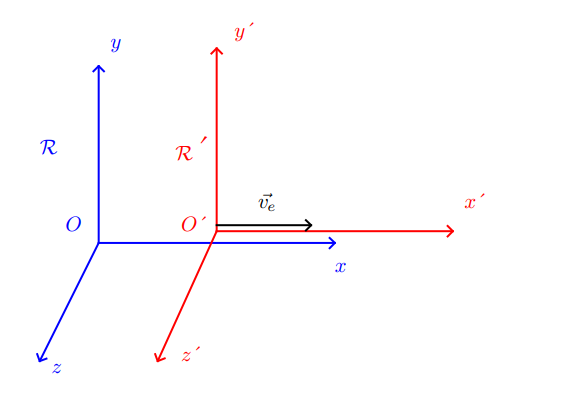
\includegraphics[width=.5\textwidth]{refgalileen.png}
% 	\caption{Référentiels en translation l'un par rapport à l'autre}
% \end{figure}

Dans ce contexte on définit une transformée pour passer des coordonnées d'un référentiel $\mathcal{R}$ à un autre $\mathcal{R}'$. On prend ces deux référentiels tels que à $t=0$, ils sont confondus, les horloges sont synchronisées. $t>0$ $\vec{v}(O') = v_e\vec{e_x}$. On peut alors décrire la position d'un point M par rapport au référentiel $\mathcal{R}$ grâce à \textbf{la transformée de Galilée}:


\begin{equation}
	\left\{\begin{array}{rcl}
		x(t) &=& x'+v_e t\\
		y(t) &=& y'\\
		z(t) &=& z'\\
		t &=& t'
	\end{array}\right.
\end{equation}

\textbf{Resultat:Loi de composition des vitesses}
	\begin{equation}
		v = v'+v_e
	\end{equation}


\subsection*{1.2. Qu'en est-il de l'électromagnétisme ?}
Les équations de Maxwell prédisent l'existence d'ondes se propageant à la vitesse $c$ a priori dans un référentiel privilégié (celui où sont définies les équations de Maxwell).

\begin{equation}
	\Delta E = \dfrac{1}{c^2}\dfrac{\partial^2 E}{\partial t^2} \text{ avec } c=\dfrac{1}{\sqrt{\epsilon_0\mu_0}}.
\end{equation}

On peut se demander quel est ce référentiel où des ondes peuvent se propager à une vitesse constante $c=3.0\cdot10^8~\rm m\cdot s^{-1}$. Si la vitesse de la lumière est définie dans un référentiel particulier et si elle obéit à la loi de composition des vitesses, on doit pouvoir mesurer une variation de la vitesse dans un autre référentiel. C'est ce que Michelson et Morley ont essayé de faire. 

\section*{2. Expérience de Michelson et Morley}

\textbf{Objectif:} Mesurer la variatio de la célérité de la lumière et vérifier que a lumière suit la loi de composition des vitesses.

\subsection*{2.1. Dispositif}

L'idée de Michelson et Morley est de se placer dans un référentiel qui se déplace par rapport au référentiel absolu dans lequel $c$ est définie. La planète Terre est en orbite quasi-circulaire de rayon $r=1.5\cdot 10^{11}~\rm m$ autour du soleil avec une période de $T = 365~\text{jours} = 3.15\cdot 10^{7}~ \rm s$. Ce qui donne une vitesse de la Terre autour du soleil de $v=3.0\cdot 10^4~\rm m\cdot s^{-1}$.

S'il existe un référentiel absolu pour la lumière on devrait pouvoir mesurer la variation de vitesse grâce à un dispositif suffisamment précis. Michelson construit un interféromètre dont l'idée est de faire interférer deux rayons lumineux ayant parcourus deux chemins différents .

\begin{center}
	\textbf{Bien décrire le dispositif expérimental sur transparents} (parcours des rayons, lame séparatrice, miroirs, détecteur)
\end{center}

% \begin{figure}[ht]
% 	\centering
% 	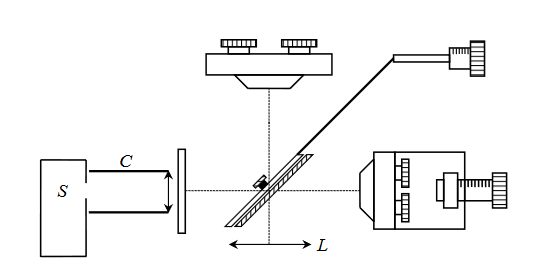
\includegraphics[width = .5\textwidth]{Michelson.png}
% 	\caption{Schéma de l'interféromètre de Michelson (\textit{Pérez, Relativité})}
% \end{figure}

L'éclairement sur le détecteur \textbf{P} dépend de $\Delta t$ le décalage temporel entre les rayons pour arriver sur le détecteur depuis la source. Les interférences dépendent de la phase : 

\begin{equation}
	\phi = 2\pi\nu\Delta t.
\end{equation}

\subsection*{2.2. Expression de la différence de phase}

On souhaite exprimer le retard d'un rayon par rapport à l'autre:

\begin{equation}
	\Delta t = T_{\parallel}-T_{\perp}
\end{equation}

On se place dans le référentiel lié au soleil et on suppose la Terre en translation rectiligne uniforme autour du soleil. L'interféromètre est placé sur Terre et se déplace à la vitesse $v_e = 3\cdot 10^4 ~\rm m\cdot s^{-1}$ par rapport au soleil. 

\subsubsection*{2.2.1. Chemin perpendiculaire:}

% \begin{figure}[ht]
% 	\centering
% 	\includegraphics[width=.5\textwidth]{schematrajetperp.png}
% 	\caption{Schéma chemin n$^\circ 1$}
% 	% \label{fig:chemin1}
% \end{figure}

On applique le théorême de Pythagore au triangle rectangle (ABC) de la figure 3:
\begin{equation}
	(ct)^2=L^2+(v_et)^2 \nonumber
\end{equation}

On factorise par le temps, le rayon issu de la lame séparatrice met un temps $t$ pour aller jusqu'au miroir $M_2$: 
\begin{equation}
	t=\dfrac{L}{c}\dfrac{1}{\sqrt{1-\left(\dfrac{v_e}{c}\right)^2}}. \nonumber
\end{equation}

En comptant le retour on en déduit $T_\perp$:
\begin{equation}
	T_\perp=2t=\dfrac{2L}{c}\dfrac{1}{\sqrt{1-\left(\dfrac{v_e}{c}\right)^2}}
\end{equation}

\subsubsection*{2.2.2. Chemin longitudinal:}
% \begin{figure}[ht]
% 	\centering
% 	\includegraphics[width=.4\textwidth]{schematrajetlongitudinal.png}
% 	\caption{Schéma chemin n$^\circ 1$}
% 	% \label{fig:chemin2}
% \end{figure}

Dans ce cas le dispositif se déplace parallèlement au rayon lumineux dont le rayon doit rattraper le miroir qui s'éloigne en même temps que le rayon avance tandis que le retour sera plus rapide car la lame semi-réfléchissante se rapproche du rayon réfléchi.

\begin{equation}
	\text{À l'aller : } t_{1} = \dfrac{L}{c+v_e}~\text{ au retour } t_2=\dfrac{L}{c-v_e}.\nonumber
\end{equation}

On en déduit $T_\parallel$:
\begin{equation}
	T_\parallel=\dfrac{2L}{c}\dfrac{1}{1-\left(\dfrac{v_e}{c}\right)^2}.
\end{equation}

Enfin, on peut exprimer le décalage temporel entre les rayons passant dans chaque bras de l'interféromètre: 

\begin{equation}
	\Delta t = T_\parallel - T_\perp = \dfrac{2L}{c}\left[\dfrac{1}{1-\left(\dfrac{v_e}{c}\right)^2}-\dfrac{1}{\sqrt{1-\left(\dfrac{v_e}{c}\right)^2}}\right]
\end{equation}

On fait le développement au premier ordre des fractions avec $v_e/c <<1$, en simplifiant les expressions il vient: 

\begin{equation}
	\Delta t = \dfrac{L}{c}\left(\dfrac{v_e}{c}\right)^2
\end{equation}

\subsection*{2.3. Résultats}

Par conséquent on peut prévoir le déphasage qu'engendre un tel décalage temporel: 
\begin{equation}
	\phi = 2\pi\dfrac{L\nu}{c}\left(\dfrac{v_e}{c}\right)^2 = 2\pi\dfrac{L}{\lambda}\left(\dfrac{v_e}{c}\right)^2.
\end{equation}

En prenant en compte les améliorations apportées par Morley à l'interféromètre de Michelson. Les bras du Michelson mesurent en comptant les réflexions $L=11~\rm m$, la longueur d'onde du Laser est de $\lambda=550~\rm m$. On trouc un déphasage 
\begin{equation}
	\dfrac{\phi}{2\pi} = 0.2
\end{equation}

Cela devrait être suffisant pour détecter un déplacement des franges de la figure d'interférence. Cependant le déplacement observé en pratique est nettement plus faible. Michelson et Morley observent un déplacement maximum de l'ordre de 0.02, en moyenne de 0.01.

% \begin{figure}[ht]
% 	\centering
% 	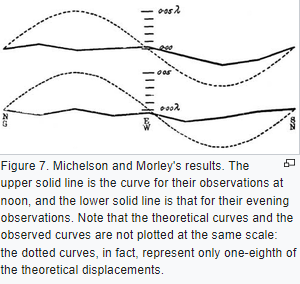
\includegraphics[width=.5\textwidth]{resultsMichelsonMorley.png}            \caption{Résultats obtenus par Michelson et Morley (\textit{Wikipedia})}
% 	% \label{fig:resMM}
% \end{figure}

\begin{definition}{Conclusion}
	On en conclut que l'on ne peut pas vérifier l'hypothèse suivant laquelle $c$ suit la loi de composition des vitesses. La mesure de la vitesse de la lumière semble indépendante du mouvement de la Terre par rapport au soleil. On peut alors prendre deux positions: 
	\begin{enumerate}
		\item Essayer de réparer la théorie du référentiel dans lequel sont définies les équations de Maxwell. 
		\item Plus courageux, admettre que $c$ est un invariant qui n'obéit pas aux lois de la cinématique galiléenne. Cela implique une nouvelle cinématique, c'est ce qu'a proposé Einstein en 1805 et que nous allons voir dans la partie suivante.
	\end{enumerate}
\end{definition}

\section*{3. Fondements de la relativité restreinte}

\subsection*{3.1. Postulats}

\begin{enumerate}
	\item Invariance des lois de la Physique
	
Toutes les lois de la physique sont invariantes par changement de référentiel galiléen. C'est à dire que les même lois se traduisent par des relations qui gardent la même structure au passage à un autre référentiel.
	\item Invariance de la vitesse de la lumière
	
Les équations de Maxwell sont invariantes par changement de référentiel. La célérité de la lumière est un invariant relativiste par changement de référentiel.

\begin{definition}{Définition - Célérité de la lumière}
	\begin{equation}
		c = \dfrac{1}{\sqrt{\epsilon_0\mu_0}}=3.0\cdot 10^8~\rm m\dot s^{-1}.
	\end{equation}
\end{definition}

À ce stade on peut revenir sur l'expérience de Michelson et Morley, car si $c=\rm constante$ alors il $\Delta t = 0$.

	\item Transformation de Lorentz poincaré
\begin{definition}{Définition - Transformée de Lorenz}
	\begin{equation}
		\left\{\begin{array}{rcl}
			ct &=& \gamma\left(ct'+\beta x'\right)\\
			x &=& \gamma\left(x'+\beta ct'\right)\\
			y &=& y'\\
			z &=& z'
		\end{array}\right.
	\end{equation}
\end{definition}	
\end{enumerate}

\subsection*{3.2. L'espace et le temps}


\subsubsection*{3.2.1. Notions d'évènements}

Le temps n'est plus un invariant, on ne peut plus le séparer des coordonnées spatiales. Il faut décrire les expériences en termes d'évènements : "Il s'est passé quelque chose quelque part" comme par exemple allumage d'une lampe sur l'ISS. Les évènements sont indépendants du référentiel.

\subsubsection*{3.2.2. Représentation spatiale}

% \begin{figure}[ht]
% 	\centering
% 	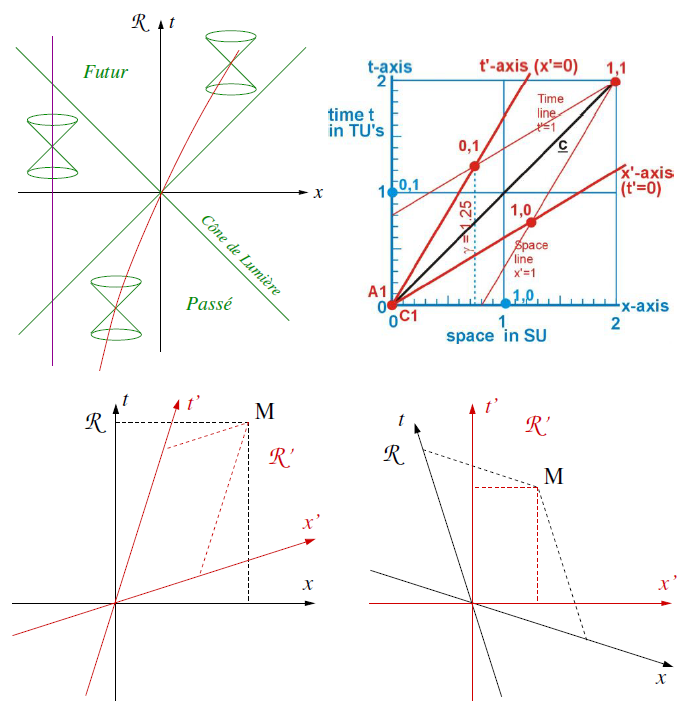
\includegraphics[width=.5\textwidth]{Minkowski.png}
% 	\caption{Diagramme espace-temps (diagramme de Minkowski)}
% \end{figure}

Deux évènements sont séparés par ce que l'on appelle l'intervalle, notée $\Delta s$. 

\begin{equation}
	\Delta s = c^2t^2-x^2-y^2-z^2
\end{equation}

L'intervalle est un invariant par changement de référentiel: $\Delta s = \Delta s'$. (commenter les valeurs de $\Delta s$ sur le graphique)

\subsection*{3.3. Conséquences de la relativité restreinte. Application au paradoxe du train et du tunnel (exercice)}

\textbf{Énoncé:} On a un train de longueur $L'$ mesuré dans $\mathcal{R}'$ (référentiel lié au train) animé d'une vitesse $\vec{v}=0.54c\vec{e}_x$ par rapport au référentiel $\mathcal{R}$ lié au tunnel (de longueur $L$ dans $\mathcal{R}'$). Le train rentre dans le tunnel rectiligne lors de l'évènement $A_1$. On prendra cet évènement comme origine spatiale et temporelle pour cet exercice où les deux référentiels sont confondus. On définit les évènements suivants:

\begin{itemize}
	\item $A_1$: l'avant du train rentre dans le tunnel : $\begin{pmatrix}
		x_{A_1}\\
		ct_{A_1}
	\end{pmatrix}_{\mathcal{R}} = \begin{pmatrix}
		0\\
		0
	\end{pmatrix}=\begin{pmatrix}
		x'_{A_1}\\
		ct'_{A_1}
	\end{pmatrix}_{\mathcal{R}'} $

	\item $A_2$: l'arrière du train entre dans le tunnel : $\begin{pmatrix}
		x_{A_2}\\
		ct_{A_2}
	\end{pmatrix}_{\mathcal{R}}$

	\item $B_1$: l'avant du train sort du tunnel : $\begin{pmatrix}
		x_{B_1}\\
		ct_{B_1}
	\end{pmatrix}_{\mathcal{R}}$

	\item $B_2$: l'arrière du train sort du tunnel : $\begin{pmatrix}
		x_{B_2}\\
		ct_{B_2}
	\end{pmatrix}_{\mathcal{R}} $
\end{itemize}

% \begin{figure}[ht]
% 	\centering
% 	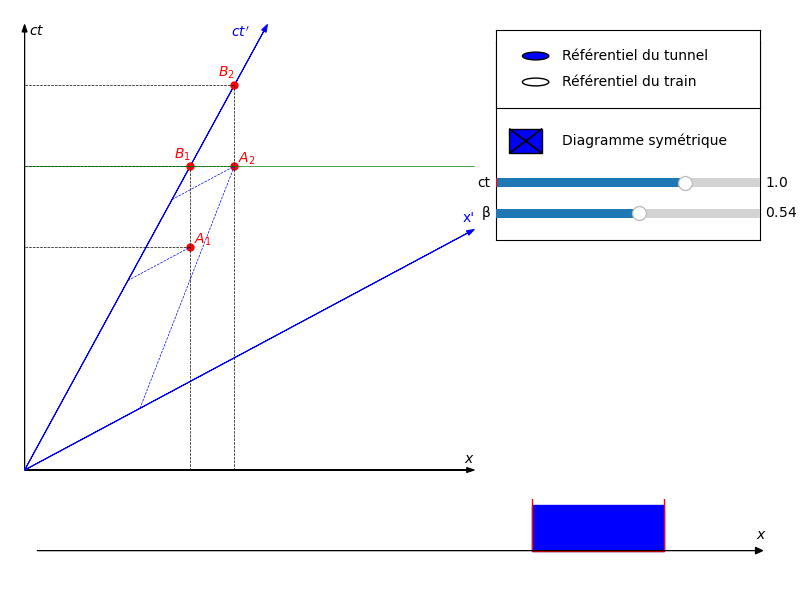
\includegraphics[width = .5\textwidth]{TrainEinstein.png}
% 	\caption{Simulation du paradoxe du train à discuter avec les calculs suivants}
% \end{figure}

\subsubsection*{3.3.1. Relativitié simultanéité}

Si nous disons que le train à 7h précise du matin sera complètement dans le tunnel, \textit{i.e.} $ct_{A_2}=ct_{B_1}$ dans le référentiel de l'observateur lié au tunnel. Dans le cadre de la relativité galiléenne où le temps est un invariant, dans le référentiel $\mathcal{R}'$ du train on aura aussi $t = t'$.

En cinématique relativiste ce n'est pas vrai: 

\begin{equation}
	\begin{array}{rcl}
	ct'_{A_2}-ct'_{B1} &= \gamma\left(ct_{A_2}-\beta x_{A_2}\right)-\gamma\left(ct_{B_1}-\beta x_{B_1}\right)\\
	&= \gamma\left(ct_{A_2}-ct_{B_1}\right)-\gamma\beta\left(x_{A_2}-x_{B_1}\right)\\
	&= \gamma\beta L
	\end{array}
\end{equation}

Les deux évènements simultanés dans $\mathcal{R}$ ne le sont pas dans $\mathcal{R}'$. (Le montrer à l'aide de la simulation).

\subsubsection*{3.3.2. Relativitié simultanéité}

Dans $\mathcal{R}'$ le trains mesure une longueur $L'$ c'est la longueur propre du train dans son référentiel propre. On peut mesurer sa taille dans le référentiel du tunnel. 

\begin{equation}
	\begin{array}{rcl}
		L'  &= x'_{A_2}-x'_{B_1}\\
            &= \gamma(x_{A_2}-\beta ct_{A_2})-\gamma(x_{B_1}-\beta ct_{B_1})\\
		    &= \gamma(x_{A_2}-x_{A_1})-\beta\gamma(ct_{A_2}-ct_{B_1})\\
		L'&= \gamma L
	\end{array}
\end{equation}

On en déduit que la longueur du train dans $\mathcal{R}$ est plus petite que dans $\mathcal{R}'$ (Le montrer à l'aide de la simulation).

\subsubsection*{3.3.3. Dilatation du temps}

Pour deux évènements, on peut établir la relation entre le temps propre et le temps mesuré dans un autre référentiel à condition que $x'2=x'1$ comme par exmpe pour les évènements $A_1$ et $B_1$.

On calcule : 

\begin{equation}
	\begin{array}{rcl}
		ct_{B_1}-ct_{A_1} &=& \gamma(ct'_{B_1}-ct'_{A_1})\\
		T_{\rm impropre} &=& \gamma T_{\rm propre}.
	\end{array}
\end{equation}

\subsection*{3.4. Loi de composition des vitesses}

\begin{equation}
	\left\{\begin{array}{rcl}
		ct &=& \gamma\left(ct'+\beta x'\right)\\
		x &=& \gamma\left(x'+\beta ct'\right)\\
		y &=& y'
	\end{array}\right.\leftrightarrow \left\{\begin{array}{rcl}
		dt &=& \gamma\left(dt'+\dfrac{v_e}{c^2} dx'\right)\\
		dx &=& \gamma\left(dx'+v_e dt'\right)\\
		dy &=& dy'
	\end{array}\right. \nonumber
\end{equation}

On obtient les vitesses en dérivant les coordonnées spatiales par rapport au temps : 
\begin{equation}
	\left\{\begin{array}{rcl}
		v_x = \dfrac{dx}{dt} &=& \dfrac{v_x'+v_e}{1+v_e\dfrac{v_x'}{c^2}}\\
		v_y = \dfrac{dy}{dt} &=& \dfrac{v_y'}{\gamma(1+v_e\dfrac{v_x'}{c^2})}
	\end{array}\right.
\end{equation}

\section*{Conclusion}

Pour ce premier cours de relativité restreinte, nous avons établi les bases d'une nouvelle cinématique. Il faut maintenant établir une nouvelle dynamique. Ainsi dans un prochain cours nous mettrons en équation la dynamique relativiste, en particulier nous écrirons les quadrivecteurs énergie et impulsion pour une particule en mouvement.

\clearpage

\section*{Leçon 27: Effet tunnel, application à la réactivité alpha}

\hrulefill\\

\noindent\underline{\textbf{Niveau:}} 
\begin{itemize}
    \item Deuxième année CPGE
\end{itemize}

\noindent\underline{\textbf{Pré-requis:}}
\begin{itemize}
    \item Physique ondulatoire
    \item Notion de mécanique quantique (eq de Schrödinger stationnaire, puits de potentiels)
    \item radioactivité
\end{itemize}

\noindent\underline{\textbf{Références:}}

\begin{itemize}
    \item Dunoc PC 
    \item Berkley quantique
    \item 51 leçons pour l'agreg
    \item sujet des mines
\end{itemize}

\hrulefill


\section*{Introduction}

Avec le puit de potentiel et la barrière de potentiel, on a vu que la fonction d'onde pouvait déborder sur des zones ou le potentiel est plus grand que son énergie. On peut le montrer via un programme python, par exemple avec la marche que l'on peut trouver en exercice (exo 34.6 Dunod PC 2019 par exemple). Ou comme dans le dunod avec un puit de potentiel carré.\medskip

On a vu dans le cours précédent qu'une particule quantique dans un puit de potentiel fini présente des niveaux d'énergie qui sont quantifiés:
\begin{equation}
    E_n = n^2\dfrac{k^2\hbar^2}{2m}
\end{equation}

où $n$ est le $n-ème$ état quantique de la particule tel que $n=1$ est le fondamental. $a$ est la largeur du puit de potentiel. $\hbar$ la constante de Planck et $m$ la masse de la particule. La recherche des fonctions d'ondes propres vérifiant Schrödinger stationnaire conduit à la recherche de mode propres de vibration (un peu comme la corde de Melde).Utiliser l'analogie de la corde de Melde que les étudiants connaissent.  Dans les deux cas l'écriture des conditions aux limites impose une quantification des vecteurs d'ondes  et revient à écrire $a=n\lambda_n/2$.  On présente alors le programme python Du puit carré. On peut présenter les trois premiers états par exemple.\medskip

On pourrait sortir une corde de Melde pour le montrer qualitativement mais ce n'est pas l'objet de la leçon et pas le temps. Noeuds = densité de probabilité nulle, ventres = densité de proba maximale.

Pour une particule classique, les zones pour $|x|>a/2$ sont interdites. En revanche on remarque que pour une particule quantique, la probabilité d'obtenir une particule au-delà de la barrière est non nulle ! L'expression de la fonction d'onde dans les zones I et III (zone interdite) sont de la forme :

\begin{equation}
    \psi(x) = A{\rm e}^{\pm qx}
\end{equation}

C'est l'expression d'une onde évanescente, dont on peut définir une profondeur de pénétration de la particule quantique d'énergie $E<V_0$ dans les régions interdites par la mécanique classique:

\begin{equation}
    \delta = \dfrac{\hbar}{\sqrt{2m(V_0-E)}}
\end{equation}

Comment peut-on utiliser cette propriété ? 

\section*{1. Barrière de potentiel}

\subsection*{1.1. Fonction d'onde prore}
On suit le Dunod PC p $1261$, on résoud Schrödinger stationnaire dans les trois domaines donnés.


Probabilité : $|\psi(x,t)|^2dx$ = probabilité de trouver la particule entre x et x+dx. Interprétation possible que si $\int_{-\infty}^{+\infty}|\psi(x,t)|^2dx=1$.\\

Equation de Schrodinger : $i\hbar\frac{\partial \psi(x,t)}{\partial t}=-\frac{\hbar^2}{2m}\frac{\partial^2\psi(x,t)}{\partial x^2}+V(x)\psi(x,t)$\\

Equation linéaire, on peut choisir $\psi = \chi(x)\exp\left(-\frac{iE}{h}t\right)$ avec le signe - dans l'exponentiel pour faire correspondre l'énergie de la particule.\\

Energie = valeur propre de H, c'est ce qu'on cherche à résoudre tout le temps en mécanique quantique. 
\begin{itemize}
    \item Si V confinement $V\sim x^2$, alors E est quantifié. on a des \textbf{états liés}
    \item Si V non confinement, E est continue et on a des \textbf{états de diffusion (ou libres)}
\end{itemize}

Etats de diffusion : ce sont les états qui vont nous intéresser pour l'effet tunnel. Comment les interpréter ?


\subsection*{1.2. Probabilité de réflexion et de transmission. Effet tunnel}

Toujours Dunod PC. On donne les fonctions d'ondes incidentes et réfléchies ainsi que les vecteurs densités de proba. Pour arriver a définir les coefficients de réflexion et transmission.

\begin{equation}
    \begin{array}{lll}
        R = \dfrac{||\vec{j}_r||}{||\vec{j}_i||}& \text{ et }& T=\dfrac{||\vec{j}_t||}{||\vec{j}_i||}
    \end{array}
\end{equation}

On écrit les conditions aux limites pour déterminer les coefficients. On en déduit $R$ et $T$.

\subsection*{1.3. Approximation d'une barrière épaisse}

On s'intéresse au cas d'une barrière épaisse, c'est à dire que sa largeur a est très grande devant la profondeur de pénétratin $a\ll \delta$. Cela correspond à $a$ grand ou $V_0 \ll E$. (particules de faible énergie devant la hauteur de la barrière).   On peut alors simplifier l'expression de $T$ car $\sinh(qa)\sim {\rm e}^{2qa}/4\ll 1$. Le coefficient de transmission devient : 

\begin{equation}
    T\approx \dfrac{16E(V_0-E)}{V_0^2}{\rm e}^{-2qa}
\end{equation}

On peut donner en transparents différents ordres de grandeurs pour différentes particules. On choisit d'étudier la radioactivité $\alpha$.

\section*{2. Radioactivité $\alpha$}



\subsection*{2.1. Description et résultats expérimentaux}
Phénomène naturel qui résulte de l 'instabilité d'un noyau atomique qui se désintègre (DUNOD PC 2019 p 1271). Rappeler que c'est l'emission d'une particule $\alpha$ par un noyau instable. Il s'agit d'un noyau d'Helium très stable (2 protons et 2 Neutrons). On peut donner en transparents des exemples de désintégration (Uranium ou radium par exemple).

On peut montrer les résultats expérimentaux \url{https://link.springer.com/article/10.1140/epja/i2019-12804-5}

On constate que le temps de demi-vie est d'autant plus court que l'éergie cinétique de la particule est grande on expliquera ce temps de demi-vie grâce à l'effet tunnel.

\subsection*{2.2. Théorie de la radioactivité $\alpha$: Gamoz Gurney et Condon (BUP 734, MINES PC 2016)}


La radioactivité $\alpha $ a été interprété en 1928 par Gamow grâce à l'effet tunnel. Il considère que le noyau X était constitué au préalable de la particule $\alpha$ et du noyau Y. L'énergie potentielle $V(x)$ (interaction forte de courte portée et de la répulsion électrostatique) entre les deux particules est une fonction de la distance qui les sépare. À l'extérieur c'est le potentiel de Coulomb qui s'applique à la particule. Dessiner le profil du potentiel.\medskip

On mène les calculs comme sur le corrigé des mines. On remarque que la particule $\alpha$ devrait rester piégée dans le puit. Elle s'explique par l'existence d'un effet tunnel: la particule doit travers la barrière par effet tunnel sur une distance. On calcule cette distance ppour l'énergie indiquée dans le tableau de l'article.

On arrive ensuite à l'expression de $\ln{T}$

\subsection*{2.3. Détermination du temps de vie}

On connaît l'expression du coefficient de transmission T. On approxime la barrière variant continument par plusieurs barrières rectangulaires. Le coefficient de transmission global  est le produit des coefficients de transmission. 

\begin{equation}
    \ln(T)=a-\dfrac{b}{\sqrt{E}}
\end{equation}

On constate que T décroit lorsque E augmente ou lorsque la masse decroit. La particule fait des allers-retours dans le noyau et ne cesse de rebondir contre la barrière de potentiel. À chaque collision elle a une proba d'être transmise T. 

Entre deux rebonds sur la barrière, la particule parcours la distance $4x_0$. Donc $t_m = 4x_0/v$. Le nombre moyen de rebonds par seconde:

$$N=1/t_m$$

et la probabilité d'émission $\alpha$ s'écrit $$dp=NTdt = \dfrac{T}{t_m}dt$$

Soit la variation du nombre de noyaux $$dN=-Ndp=-N\dfrac{T}{t_m}dt$$

Soit $$N(t) = N_0{\rm e}^{-Tt/tm}$$

La demi-vie est définie comme le temps après lequel la moitié des noyaux s'est désintégré: $$N(\tau_{1/2})=\dfrac{N_0}{2}$$
Donc $$\tau_{1/2}=t_m\ln{2}/T$$

 $$\ln{\tau_{1/2}}=\ln\ln 2+\ln t_m-\ln T = \underbrace{\ln\ln 2+\ln t_m-a}_{\rm constante}+\dfrac{b}{\sqrt{E}}$$

 On retrouve la loi expérimentale !  Peut-on tracer les données à partir du tableau ? 

 \section*{Conclusion}

 Effet tunnel bien utile pour comprendre des phénomènes naturel. On en a pas parlé mais il est également utilisé pour des application technologiques actuelles : microscope à effet tunnel \url{https://toutestquantique.fr/tunnel/}.


\end{document}

%%
%% FIN DU DOCUMENT
%%
